\documentclass[a4paper]{article}
%% Language and font encodings
\usepackage[english]{babel}
\usepackage[utf8x]{inputenc}
\usepackage[T1]{fontenc}
\usepackage{float}
%% Sets page size and margins
\usepackage[a4paper,top=3cm,bottom=2cm,left=3cm,right=3cm,marginparwidth=1.75cm]{geometry}

%% Useful packages

\usepackage[compat=1.1.0]{tikz-feynman}
\tikzfeynmanset{/tikzfeynman/momentum/arrow shorten = 0.3}
\tikzfeynmanset{/tikzfeynman/warn luatex = false}
\usepackage{tensor}
\usepackage{tikz}
\usepackage{fancyhdr}
\pagestyle{fancy}
\usepackage{amsmath}
\usepackage{amstext}
\usepackage{amsthm}
\usepackage{enumitem}
\usepackage{eqnarray}
\usepackage{float}
\usepackage{esint}
\usepackage{wrapfig}
\usepackage{gensymb}
\usepackage{lipsum}
\usepackage{amssymb}
\usepackage{array}
\usepackage{tikz}
\usepackage[colorlinks=true, allcolors=blue]{hyperref}
\usepackage{graphicx}
\usepackage{amsmath}
\usepackage{amssymb}

\usepackage{graphicx}
\usepackage{mathtools}
\usepackage[caption=false]{subfig}
\DeclareMathOperator{\Sym}{Sym}
\DeclareMathOperator{\Auto}{Aut}
\DeclareMathOperator{\lcm}{lcm}
\DeclareMathOperator{\Tr}{Tr}
\DeclareMathOperator{\R}{Im}
\DeclareMathOperator{\Ker}{Ker}
\DeclareMathOperator{\sech}{sech}
\DeclareMathOperator{\diag}{diag}
\DeclareMathOperator{\sgn}{sgn}
\DeclareMathOperator{\Mod}{mod}
\DeclareMathOperator{\cl}{cl}
\newcommand{\iso}{\xrightarrow{
   \,\smash{\raisebox{-0.65ex}{\ensuremath{\scriptstyle\sim}}}\,}}
\newtheorem{post}{Postulate}[section]
\newtheorem{eg}{Example}[section]
\newtheorem{remarks}{Remarks}[section]
\newtheorem{notation}{Notation}[section]
\newtheorem{Note}{Note}[section]
\definecolor{darkblue}{RGB}{	0, 0, 139}
\newtheoremstyle{new}% <name>
{2pt}% <Space above>
{2pt}% <Space below>
{\color{darkblue}}% Body font
{}% <Indent amount>
{\bfseries\color{black}}% Theorem head font
{:}% <Punctuation after theorem head>
{.5em}% <Space after theorem headi>
{}% <Theorem head spec (can be left empty, meaning `normal')>
\theoremstyle{new}
\newtheorem{law}{Law}[section]
\newtheorem{defi}{Definition}[section]
\newtheorem{thm}{Theorem}[section]
\newtheorem{prop}{Proposition}[section]
\newtheorem{lemma}{Lemma}[section]
\newtheorem{cor}{Corollary}[section]


\title{\textbf{Part II PNP Summary Notes}}
\author{Tai Yingzhe, Tommy (ytt26)}
\date{}
\setlength{\parindent}{0cm}
\begin{document}
\maketitle
{\small\tableofcontents}
\subsection*{Acknowledgements:}
Many thanks to my supervisor JingYuan Shi, and the lecturer Tina Potter for their guidance.
\newpage
\section{Fundamentals}
\subsection{Introduction}
High energy beams are necessary in particle physics to \begin{itemize}
\item probe the pointlike (elementary) constituents of matter
\item create massive elementary particles
\end{itemize}
Beams of high momentum have short de Broglie wavelengths, hence high resolution $\Delta r\approx\lambda/\sin\theta$, where $\theta$ is the angle light scatters off from the object.
\begin{eg}
In the early decades, particle-beam energies from accelerators reached only a few MeV, and their resolution was so poor that protons and neutrons could themselves be regarded as elementary and pointlike.
\end{eg}
\begin{eg}
Heaviest elementary particle detected so far is the `top' quark which has 200 times the mass-energy of a proton.
\end{eg}
\begin{eg}
The total energy in accelerator beams required to create massive elementary particles in sufficient intensities is quite substantial. An energy per particle of 1 TeV in beams consisting of bunches of $10^{13}$ accelerated particles every second will correspond to a total kinetic energy in each bunch of 1.6 MJ.
\end{eg}
\subsubsection{Elementary particles versus nuclei}
All experimental data can be practically accounted for by the Standard Model, formulated in the 1970s. The Standard Model describes the fundamental particles, the forces between them and the ways that they combine to make other particles. 
\begin{defi}[Fundamental forces]
There are four fundamental forces responsible for all observations of forces in nature. They are
\begin{itemize}
    \item gravity 
    \item strong force: binds quarks into hadrons
    \item electromagnetic force: between charged particles
    \item weak force: responsible for $\beta$-decay (radioactivity).
\end{itemize}
\end{defi}
\begin{defi}[Matter]
In the Standard Model, all matter is made of spin $1/2$ fundamental particles. There are two families - leptons ($\ell$) and quarks ($q$). Leptons are fermions which do not interact via the strong interaction, while quarks may do so. Each family has 3 generations (replicas) with two particles and two anti-particles in each. Each `flavour' of charged lepton is paired with the same `flavour' neutrino. Neutrinos are massless leptons. The table of leptons and quarks are respectively
\begin{center}
\begin{tabular}{|l|l|l|}
\hline
Gen 1   & Gen 2     & Gen 3      \\
\hline
$e$  (electron)   & $\mu$ (muon)     & $\tau$ (tauon)     \\
\hline
$\nu_e$ (electron neutrino) & $\nu_\mu$ (muon neutrino) & $\nu_\tau$ (tau neutrino)\\ 
\hline
\end{tabular}
\end{center}
\begin{center}
\begin{tabular}{|l|l|l|}
\hline
Gen 1   & Gen 2     & Gen 3      \\
\hline
$u$ (up quark)    & $c$ (charm quark)     & $t$ (top quark)    \\
\hline
$d$ (down quark) & $s$ (strange quark) & $b$ (bottom quark) \\
\hline
\end{tabular}
\end{center}
All of normal matter is made from the first generations of these families. Quarks have fractional charges and grouped into pairs differing by one unit of electric charge. 
\end{defi}
\newpage
\begin{remarks}\leavevmode
\begin{enumerate}
\item The generations are distinct. The mass of the particles increases with each generation. There is a symmetry between the generations, but the origin of 3 generations is not understood.
\item The electron, muon and tauon have a charge of $-e$, while the neutrinos are neutral. The up, charm and top quarks have a charge of $+2e/3$ while the remaining three have a charge of $-e/3$. The signs of the charges reverse for the corresponding antimatter particles.
\item Only charged leptons can interact with the electromagnetic force. All leptons experience the weak force.
\item Neutrinos were postulated in 1930 to account for the energy and momentum missing in the process of nuclear $\beta$-decay. The actual existence of neutrinos as independent particles, detected by their interactions, was first demonstrated in 1956. 
\item Strange quarks were strange in the sense that they were produced prolifically in strong interactions, and therefore would be expected to decay on a strong interaction timescale ($10^{-23}$ s); instead they decayed extremely slowly, by weak interactions. The resolution was they carried a new quantum number, $S$ for strangeness, conserved in strong interactions, and when decayed singly and weakly, they change into non-strange particles with $\Delta S=\pm1$.
\item An additional degree of freedom is needed for quarks. Each flavour of quark comes in three different colours. 
\end{enumerate}
\end{remarks}
\begin{defi}[Hadrons]
Single, free quarks have never been observed. They are always confined in bound states called hadrons. Macroscopically, hadrons behave as almost point-like composite particles. There are two types of hadrons:
\begin{itemize}
    \item mesons ($q\overline{q}$): bound states of a quark and an anti-quark and have integer spins (hence are bosons);
    \item baryons ($qqq$): bound states of three quarks with overall half-integer spins (hence are fermions).
\end{itemize}
\end{defi}
\begin{eg}\leavevmode
\begin{enumerate}
    \item Mesons: pions $\pi^+=u\overline{d}$, $\pi^-=\overline{u}d$, $\pi^0=(u\overline{u}-d\overline{d})/\sqrt{2}$ with charges $+e$, $-e$ and 0 respectively. $\pi^-$ is the antiparticle of $\pi^+$ and $\pi^0$ is its own antiparticle.
    \item Baryons: proton $p=udu$ and neutron $n=dud$ with charge $+e$ and 0 respectively. Can define the corresponding antibaryons $\overline{p}=\overline{u}\overline{d}\overline{u}$ and $\overline{n}=\overline{d}\overline{u}\overline{d}$.
\end{enumerate}
\end{eg}
\begin{defi}[Nucleus]
A nucleus is a bound state of $Z$ (atomic number) protons and $N$ neutrons. Protons and neutrons are generically referred to as nucleons. A nuclide is a specific nucleus, characterised by $Z$, $N$ and with mass number $A=Z+N$.
\end{defi}
\begin{remarks}
The strong force between nucleons is called the strong nuclear force, and it is mediated by the pion.
\end{remarks}
\begin{eg}
On the plot of $Z$ against $N$, one can define isotones and isotopes to be loci of constant $N$ and $Z$ respectively. Isobars are loci of constant $A=N+Z$.
\end{eg}
\begin{defi}[Gauge bosons]
The fundamental forces arise through the exchange of virtual field quanta called gauge bosons (with spin 1, except for graviton which has spin 2). For the four fundamental forces, their corresponding gauge bosons are
\begin{itemize}
    \item strong force: bind quarks in the neutron and proton (gluons - 8 of them), and the neutrons and protons within nuclei
    \item weak force: W$^{\pm}$ and Z bosons - responsible for radioactive decay
    \item electromagnetic force: photon - acts between charged particles
    \item gravity: graviton - acts between massive particles.
\end{itemize}
\begin{center}
\begin{tabular}{|l|l|l|l|}
\hline
Interaction   & Mediator     & $J^P$ (spin$^{\text{parity}}$) & relative strength     \\
\hline
strong   & gluon    & $1^-$ & 1     \\
\hline
electromagnetic  & photon    & $1^-$ & $10^{-2}$     \\
\hline
weak  & $W^{\pm},Z^0$   & $1^-,1^+$ & $10^{-7}$    \\
\hline
gravity  & graviton $g$    & $2^+$ & $10^{-39}$     \\
\hline
\end{tabular}
\end{center}
\end{defi}
\begin{defi}[Interaction at a distance]
In quantum theory, action at a distance is viewed in terms of an exchange interaction - the exchange of a boson associated with the particular type of interaction. 
\end{defi}
\begin{remarks}\leavevmode
\begin{enumerate}
    \item Gravity is not included in the standard model.
    \item Exchange of gauge bosons violates energy and momentum conservation, but permissible for sufficiently short times owing to the uncertainty principle, i.e. $\sigma_E\sigma_t\sim\hbar$. The larger the energy transfer (or force), the smaller the range $R\sim c\sigma_t\sim\hbar c/\sigma_E$.
    \item An unstable particle does not have a unique mass, but a distribution with `width' $\Gamma=\hbar/\tau$ where $\tau$ is the mean lifetime. When $\tau$ is very short, its value can be inferred from the measured width $\Gamma$.
    \item Since the quantum carries momentum and energy $\Delta E$, the conservation laws can only be satisfied if the process takes place within a timescale $\Delta t$ limited by the uncertainty principle. The transient exchanged particle is `virtual' and do not satisfy the mass-energy relation $E^2=p^2c^2+m^2c^4$.
    \item In the 1970s, experiments showed that the weak and electromagnetic interactions can be unified and have the same strength at very high energies. The symmetry is only broken at lower energies.
\end{enumerate}
\end{remarks}
\begin{eg}
The weak force only has a range of $10^{-18}$ m. The other fundamental forces have infinite range.  Due to quark confinement, nucleons start to experience the strong nuclear interaction at $10^{-15}$ m (femtometre).
\end{eg}
\subsubsection{Natural units}
\begin{remarks}[Energy scale]
Energies are measured in units of eV.
\begin{itemize}
    \item nuclear regime: keV to MeV
    \item particle regime: GeV to TeV
\end{itemize}
Masses are in units of MeV/c$^2$ or GeV/c$^2$. 
\end{remarks}
\begin{defi}[Natural units]
We choose $\hbar,c=1$ and so all units of measurement are some multiples of eV. We can further set other natural constants, like $\varepsilon_0$, as unity.
\end{defi}
\begin{eg}
To reintroduce `missing' factors of $\hbar$ and $c$ to convert back to SI units:
\begin{itemize}
    \item energy $\leftrightarrow$ length: $\hbar c=0.197$ GeV fm = $3.162\times10^{-26}$ J m
    \item energy $\leftrightarrow$ time: $\hbar=6.6\times10^{-25}$ GeV s
    \item length $\leftrightarrow$ time: $c=3\times10^8$ m/s
\end{itemize}
For example, cross-section is expressed as units of GeV$^{-2}$ in natural units. To convert to standard units 1 GeV$^{-2}$ is $(0.197\times10^{-15})^2=3.89\times10^{-32}$ m$^2$, which is $10^{-4}$ barns ($b$). 1 barn is $10^{-28}$ m$^2$.
\end{eg}
\begin{defi}[Heaviside-Lorentz units]
Further set $\varepsilon_0$ and $\mu_0$ to be 1. As a result, the fine structure constant (1/137) is $\alpha=\frac{e^2}{4\pi\varepsilon_0\hbar c}=\frac{e^2}{4\pi}$.
\end{defi}
\newpage
\subsection{Kinematics, decays and reactions}
\begin{notation}
We will now adopt natural units.
\end{notation}
\subsubsection{Relativistic collisions}
\begin{remarks}
Relativistic formula is necessary for particle physics where the kinetic energies are high (about 100 GeV), much larger than the rest mass energies. When a particle is ultra-relativistic ($E>>m$), then $E\sim|\vec{p}|$.
\end{remarks}
\begin{prop}
Recall from special relativity,
$$\gamma=\frac{E}{m},\quad\beta:=v=\frac{|\mathbf{p}|}{E},\quad T=(\gamma-1)m$$
\end{prop}
\begin{defi}[Lorentz invariant]
In special relativity, the inner product of any two four-vectors is a Lorentz invariant.
\end{defi}
\begin{eg}
For $(t,\mathbf{x})$, we can define the invariant interval $d^2=t^2-|\mathbf{x}|^2$. For $(E,\mathbf{p})$, we can define the invariant mass $m^2=E^2-|\mathbf{p}|^2$.
\end{eg}
\begin{defi}[Invariant mass]
For relativistic particle collisions, the invariant mass is particularly useful. For a system of particles, where X decays into $n$ particles with $(E_i,\mathbf{p_i})$, then the invariant mass is
$$M_X^2:=\bigg(\sum_{i=1}^nE_i\bigg)^2-\bigg(\sum_{i=1}^n\mathbf{p_i}\bigg)^2$$
Sometimes, the invariant mass $M$ is called the `centre of mass energy', $E_{\text{CoM}}:=\sqrt{s}$.
\end{defi}
\begin{eg}\leavevmode
\begin{enumerate}
    \item For the specific case of a two-body decay, the invariant mass reduces to 
    $$M_X^2=m_1^2+m_2^2+2(E_1E_2-|\mathbf{p_1}||\mathbf{p_2}|\cos\theta)$$
    \item Consider a charged pion decaying at rest in the lab frame $\pi^-\rightarrow\mu^-\overline{\nu}_\mu$. Invoke conservation of energy and momentum:
    $$E_\pi=E_\mu+E_\nu,\quad 0=\mathbf{p_\mu}+\mathbf{p_\nu}$$
    Since $\mathbf{p_\pi}=\boldsymbol{0}$, then $E_\pi=m_\pi$. Since $m_\nu=0$, we have $p_\nu=E_\nu$, hence
    $$(m_\pi-E_\mu)^2=E_\nu^2=|\mathbf{p_\nu}|^2=|\mathbf{p_\mu}|^2\implies m_\pi^2+E_\mu^2-2m_\pi E_\mu=p_\mu^2\implies E_\mu=\frac{m_\pi^2+m_\mu^2}{2m_\pi}$$
\end{enumerate}
\end{eg}
\subsubsection{Decays and reactions}
\begin{defi}[Particle decay]
Particle decay is the spontaneous process of one unstable subatomic particle transforming into multiple other particles. The allowed/forbidden decays are dictated by the conservation laws.
\end{defi}
\begin{remarks}
The term is typically distinct from radioactive decay, in which an unstable atomic nucleus is transformed into a lighter nucleus accompanied by the emission of particles or radiation, although the two are conceptually similar and are often described using the same terminology. The units of radioactivity are defined as the number of decays per unit time: 1 Bq (Becquerel) and 1 Ci (Curie) are respectively 1 decay per second and $3.7\times10^{10}$ decays per second.
\end{remarks}
\begin{defi}[Mean lifetime]
The mean lifetime of a decaying state is $\tau=1/W$ where $W$ is the rate of reaction. For strong decays, $\tau$ is unmeasurably short and instead one quotes the width $\Gamma$, i.e. the natural spread in energy of the decaying state, where
$$\Gamma=\frac{\hbar}{\tau}=\hbar W$$
\end{defi}
\begin{remarks}
Since $\hbar=1$, we sometimes refer to $\Gamma$ and $W$ to be the same.
\end{remarks}
\begin{prop}
Assuming a first-order decay, we have
\begin{itemize}
    \item the number of particles remaining at time $t$ to be $N(t)=N(0)e^{-\lambda t}$, where $N(0)$ is the number at time $t=0$
    \item the rate of decays at time $t$ to be $\frac{dN}{dt}=-\lambda N(t)$
    \item the activity at time $t$ is $A(t)=|\frac{dN(t)}{dt}|=\lambda N(t)$
    \item the half-life is $\tau_{1/2}=\frac{\ln 2}{\lambda}=\ln 2~\tau$, where $\tau$ is the mean lifetime.
\end{itemize}
\end{prop}
\begin{remarks}
Decaying states do not correspond to a single energy. By the uncertainty principle, the finite lifetime corresponds to an energy width of $\sigma_E\sim\hbar/\tau=\hbar\lambda$.
\end{remarks}
\begin{eg}
Decay chains frequently occur in nuclear physics, where a parent particle decays into a daughter particle, which in turn decays to a granddaughter particle. The activity of the daughter is $\lambda_2N(t)$ for $N_1\rightarrow N_2\rightarrow\dots$ and the rate of change of the daughter's population is $\frac{dN_2(t)}{dt}=\lambda_1N_1(t)-\lambda_2N_2(t)$.
\end{eg}
\begin{prop}[Fermi's Golden Rule]
The transition rate (for a particle to decay from one quantum state to another) is given by the Fermi's Golden rule
$$\Gamma(i\rightarrow f)=2\pi|\mathcal{M}_{\text{fi}}|^2\rho(E_f)$$
where $\rho(E_f)$ is the density of the final states, and $\mathcal{M}_{\text{fi}}$ is the transition matrix element. $\lambda dt$ is the probability a particle will decay in time $dt$.
\end{prop}
\begin{proof}
See Part II AQP.
\end{proof}
\begin{defi}[Resonance]
Broad states with finite widths and lifetimes, which can be formed by collision between the particles into which they decay, are referred to as resonances. 
\end{defi}
\begin{prop}
Consider a state formed at $t=0$ with energy $E_0$ and mean lifetime $\tau$, then the probability of producing the decaying state with energy $E$ is
$$P(E)\propto\frac{1}{(E_0-E)^2+(1/4\tau^2)}$$
which has a Lorentzian (or Breit-Wigner) shape, with total width equal to $\lambda=1/\tau$.
\end{prop}
\begin{proof}
Consider a state formed at $t=0$ with energy $E_0$ and mean lifetime $\tau=1/\Gamma$
$$\psi(t)=\psi(0)e^{-iE_0t}e^{-t/2\tau}\implies|\psi(t)|^2=|\psi(0)|^2e^{-t/\tau}$$
The frequencies present in the wavefunction are given by the Fourier transform of $\psi(t)$, i.e.
$$f(E)=\int_0^\infty\psi(t)e^{iEt}dt=\int_0^\infty\psi(0)e^{-t(i(E_0-E)+(1/2\tau)}dt=\frac{i\psi(0)}{(E_0-E)-(i/2\tau)}$$
The probability is $P(E)=|F(E)|^2$. The full-with at half-maximum, $\frac{1}{2}P(E=E_0)=P(E=E_0\pm0.5\Gamma)\propto\frac{1}{0.25\Gamma^2+(1/4\tau^2)}$, where $P(E=E_0)\propto 4\tau^2$. The total width is then $\Gamma=1/\tau$.
\end{proof}
\begin{remarks}\leavevmode
\begin{enumerate}
    \item The exponential decay rate determines the form of the line shape of the resonance: the energy dependence of the cross-section for creating the resonant state from its constituents is simply the Fourier transform of the time pulse.
    $$\int\psi(t)e^{i\omega t}dt=\int\psi(0)e^{-t(iE_0+\Gamma/2)}~e^{iEt}dt\propto\frac{1}{(E-E_0)-i\Gamma/2}$$
    \item Particles can often decay with more than one decay mode, each with its own transition rate. The total decay rate (and hence total width of the particle state) is the sum of the individual transition rates.
\end{enumerate}
\end{remarks}
\begin{defi}[Branching fraction]
The branching fraction is the proportion of decays to a particular decay mode is called the branching ratio $B_f=\Gamma_f/\Gamma$, such that $\sum_fB_f=1$.
\end{defi}
\newpage
\subsubsection{Cross-section}
Consider a two-body to two-body reaction of the form
\begin{equation}
a+b\rightarrow c+d\label{2body}
\end{equation}
\begin{defi}[Crossed reactions]
The crossed reactions ae obtained by replacing the incoming (outgoing) particles by outgoing (incoming) anti-particles. They are described by the same matrix element, but have different kinematic constraints., 
\end{defi}
\begin{defi}[Crossing symmetry]
Any particles of a reaction can be `crossed' over to the other side of the equation, provided it is turned into its antiparticle, and the resulting interaction will also be allowed. This is different from the `reverse reaction'.
\end{defi}
In Eqn.~\ref{2body}, a well-defined parallel beam of particles of type a impinges normally on a target of thickness $dx$ containing $n_b$ particles of type $b$ per unit volume, and $c$ and $d$ are the product particles. 
\begin{defi}[Particle flux]
If the density of particles in the incident beam is $n_a$, the flux through the target will be
\begin{equation}
    \Phi=n_av_i
\end{equation}
where $v_i$ is the velocity of the incident beam relative to the target. 
\end{defi}
\begin{defi}[Cross-section]
The strength of a particular reaction between two particles is specified by the interaction cross-section. the cross-section is the effective target area presented to the incoming particle for it to cause the reaction. $\sigma$ is defined as the reaction rate per target particle $\Gamma$ per unit incident flux $\Phi$, $\Gamma=\Phi\sigma$. The unit of cross-section is the barn 1 b$=10^{-28}$ m$^2$. \\[5pt]
If each of the target particles (b in Eqn.~\ref{2body}) has an effective cross-section $\sigma$, the probability that any particle a will hit a target particle is $\sigma n_bdx$, since this is the fraction of the target area obscured by the b particles, the number of reactions per unit time is $\Phi\sigma n_bdx$.
\end{defi}
\begin{prop}
Consider a beam of particles incident upon a target (of $n$ nuclei per unit volume, of target thickness $dx$ small), the number of particles scattered per unit time is $-dN$. The cross-section is
$$\sigma=\frac{-dN}{nN~dx}$$
\end{prop}
\begin{proof}
Referring to Eqn.~\ref{2body}, there is a beam of $N_a$ particles per unit time in an area $A$. The number of target particles in area $A$, $N_T=n_bAdx$. The effective area for absorption is $\sigma N_T$. The incident flux is $\Phi=N_a/A$. The number of particles scattered per unit time is $-dN=\Phi\sigma N_T=\frac{N_a}{A}\sigma n_bAdx$, then we have $\sigma=-\frac{dN_a}{n_bN_adx}$.
\end{proof}
\begin{remarks}
The beam attenuates exponentially in a target of thickness $L$. The mean free path between interactions is $1/n\sigma$, and defines the interaction length.
\end{remarks}
\begin{cor}
The differential cross-section is the number of particles scattered per unit time and solid angle, divided by the incident flux and by the number of target nuclei $N_T=nAdx$, defined by the beam area $A$. 
$$\frac{d\sigma}{d\Omega}=\frac{dN_{d\Omega}}{\Phi N_T d\Omega}$$
\end{cor}
\begin{proof}
The number of particles scattered per unit time into $d\Omega$ is $dN_{d\Omega}=\Phi N_Td\sigma$.
\end{proof}
\begin{remarks}
Most experiments do not cover $4\pi$ solid angle, and in general we measure $d\sigma/d\Omega$. Angular distributions provide more information than the total cross-section about the mechanism of the interaction, e.g. angular momentum.
\end{remarks}
\begin{defi}[Elastic and inelastic scattering]
Inelastic scattering occurs if the final state is not the same as the initial state. Elastic scattering occurs if the state is not changed, but only their momenta.
\end{defi}
\begin{defi}[Partial cross-sections]
 If we have different final states for the same initial states, then we can define a different partial cross-section for each final state. The total cross-section is $\sigma_{\text{tot}}=\sum_i\sigma_i$.
\end{defi}
\begin{prop}[Born approximation]
Consider a beam of relativistic particles scattering from a fixed potential $V(\mathbf{r})$
$$\frac{d\sigma}{d\Omega}=\frac{E^2}{(2\pi)^2}\bigg|\int e^{-i\mathbf{q}\cdot\mathbf{r}}V(\mathbf{r})d^3\mathbf{r}\bigg|^2$$
where $\mathbf{q}=\mathbf{p_f}-\mathbf{p_i}$ is the momentum transfer. 
\end{prop}
\begin{proof}
Consider plane wave solutions of the form $\psi\sim e^{-i(Et-\mathbf{p}\cdot\mathbf{r})}$ with normalization factor $1/L^{3/2}$ for a box geometry of side $L$. The matrix element is
$$\mathcal{M}_{\text{fi}}=\frac{1}{L^3}\int e^{-i\mathbf{p_f}\cdot\mathbf{r}}V(\mathbf{r})e^{i\mathbf{p_i}\cdot\mathbf{r}}d^3\mathbf{r},\quad\mathbf{q}=\mathbf{p_f}-\mathbf{p_i}$$
By Fermi's Golden Rule, the reaction rate is $\Gamma=\frac{2\pi}{\hbar}|\mathcal{M}_{if}|^2\rho(E_f)$, where $\rho(E_f)$ is the energy density of the final states. Consider a target of area $A$ and a beam of particles travelling at velocity $v_i$ towards the target. Any incident particle within a volume $v_iA$ will cross the target area per second. The flux is 
$$\Phi=\frac{v_iA}{A}n=v_in$$
where $n$ is the number density of incident particles which is 1 per $L^3$. For a box of side $L$, states are given by the periodic boundary conditions and hence each state occupies a volume $(2\pi/L)^3$ in phase space. In phase space, the number of states between $p$ and $p+dp$ in solid angle $d\Omega$ is
$$dN=\bigg(\frac{L}{2\pi}\bigg)^3p^2dpd\Omega\implies\rho(p)=\frac{dN}{dp}=\bigg(\frac{L}{2\pi}\bigg)^3p^2d\Omega$$
The density of states in energy $E^2=p^2+m^2\implies\frac{dE}{dp}=\frac{p}{E}$. Hence
$$\rho(E)=\frac{dN}{dE}=\frac{dN}{dp}\frac{dp}{dE}=\bigg(\frac{L}{2\pi}\bigg)^3p^2\frac{E}{p}d\Omega$$
For relativistic scattering, we have $E\sim p$. Putting everything together
$$d\sigma=\frac{1}{\Phi}2\pi|\mathcal{M}_{\text{fi}}|^2\rho(E_f)=\frac{L^3}{v_i}2\pi\bigg|\frac{1}{L^3}\int e^{-i\mathbf{q}\cdot\mathbf{r}}V(\mathbf{r})d^3\mathbf{r}\bigg|^2\bigg(\frac{L}{2\pi}\bigg)^3p_fE_fd\Omega\implies\frac{d\sigma}{d\Omega}=\frac{1}{(2\pi)^2v_i}\bigg|e^{-i\mathbf{q}\cdot\mathbf{r}}V(\mathbf{r})d^3\mathbf{r}\bigg|^2p_fE_f$$
where $v_i\sim c=1$ in natural units and we obtain our desired result.
\end{proof}
\begin{eg}[Rutherford scattering]
Consider relativistic elastic scattering in a Coulomb potential $V(r)=-\frac{Z\alpha}{r}$. The matrix element is 
$$|\mathcal{M}_{\text{fi}}|^2=\frac{16\pi^2Z^2\alpha^2}{q^4}=\frac{16\pi^2Z^2\alpha^2}{(4E^2\sin^2(\theta/2))^2}$$
where $|\mathbf{q}|^2=|\mathbf{p_i}|^2+|\mathbf{p_f}|^2-2\mathbf{p_i}\cdot\mathbf{p_f}=2|\mathbf{p}|^2(1-\cos\theta)=4E^2\sin^2(\theta/2)$ since for elastic scattering, we have $|\mathbf{p_i}|^2=|\mathbf{p_f}|^2$. By Born's rule, the differential cross-section is
$$\frac{d\sigma}{d\Omega}=\frac{4E^2Z^2\alpha^2}{q^4}=\frac{4E^2Z^2\alpha^2}{16E^4\sin^4(\theta/2)}=\frac{Z^2\alpha^2}{4E^2\sin^4(\theta/2)}$$
\end{eg}
\newpage
\subsubsection{Resonant scattering}
\begin{defi}[Resonant state]
Some particle interactions take place via an intermediate resonant state, which in turn decays.
\end{defi}
\begin{defi}[Bohr model]
For the resonant scattering
$$a+b\rightarrow Z^*\rightarrow c+d$$
In the Bohr model, we consider the two stages separately:
\begin{itemize}
    \item formation: $a+b\rightarrow Z^*$ which occurs when the collision energy $E_{\text{CoM}}$ equals to the natural frequency of a resonant state
    \item decay: $Z^*\rightarrow c+d$ which occurs independently on the mode of formation, and only depends on the properties of the $Z^*$.
\end{itemize}
\end{defi}
\begin{prop}[Breit-Wigner cross-section]
\begin{equation}
\sigma=\frac{\pi g}{p_i^2}\frac{\Gamma_{Z\rightarrow i}\Gamma_{Z\rightarrow f}}{(E-E_0)^2+(\Gamma^2/4)}\label{BreitWigner}
\end{equation}
where $g$ is the spin multiplicity factor.
\end{prop}
\begin{proof}
The resonance cross-section is given by
$$d\sigma=\frac{1}{\Phi}2\pi|\mathcal{M}_{\text{fi}}|^2\rho(E_f)=\frac{L^3}{v_i}2\pi|\mathcal{M}_{fi}|^2\bigg(\frac{L}{2\pi}\bigg)^3p_F^2\frac{E}{p_f}d\Omega$$
where we have the incident flux to be $\Phi=v_i/L^3$ and $E/p=1/v$.  The factors of $L$ cancel from the normalization in $|\mathcal{M}_{\text{fi}}|^2$, giving $\frac{d\sigma}{d\Omega}=\frac{p_F^2}{(2\pi)^2v_iv_f}|\mathcal{M}_{\text{fi}}|^2$. The matrix element is given by the second order perturbation theory:
$$\mathcal{M}_{\text{fi}}=\sum_Z\frac{\mathcal{M}_{iZ}\mathcal{M}_{Zf}}{E-E_Z}$$
where the sum runs over all intermediate state. Near resonance, effectively only one state Z contributes. Consider one intermediate state described by $\psi(t)=\psi(0)e^{iE_0t}e^{-t/2\tau}=\psi(0)e^{-i(E_0-i0.5\Gamma)t}$, which describes a state with energy $E_0-i0.5\Gamma$, then 
$$|\mathcal{M}_{\text{fi}}|^2=\frac{|\mathcal{M}_{iZ}^2|\mathcal{M}_{Zf}|^2}{(E-E_0)^2+0.25\Gamma^2}$$
The rate of decay and formation of Z are respectively
$$\Gamma_{Z\rightarrow f}=2\pi|\mathcal{M}_{Zf}|^2\rho(E_f)=2\pi|\mathcal{M}_{Zf}|^2\frac{4\pi p_f^2}{(2\pi)^3v_f}=|\mathcal{M}_{Zf}|^2\frac{p_f^2}{\pi v_f},\quad\Gamma_{i\rightarrow Z}=|\mathcal{M}_{iZ}|^2\frac{p_i^2}{\pi v_i}$$
Putting everything together gives
$$\sigma=4\pi\frac{p_f^2}{(2\pi)^2v_iv_f}\frac{1}{(E-E_0)^2+0.25\Gamma^2}\frac{\pi v_f}{p_f^2}\Gamma_{Z\rightarrow f}\frac{\pi v_i}{p_i^2}\Gamma_{Z\rightarrow i}=\frac{\pi}{p_i^2}\frac{\Gamma_{Z\rightarrow i}\Gamma_{Z\rightarrow f}}{(E-E_0)^2+0.25\Gamma^2}$$
Finally, we have to account for the spin states of  a and b, i.e. the probability that the initial states a and b collide in the correct spin states to form $Z^*$, i.e. $g=\frac{2J_Z+1}{(2J_a+1)(2J_b+1)}$.
\end{proof}
\begin{remarks}\leavevmode
\begin{enumerate}
    \item $p_i$ is calculated in the centre of mass frame and it is the momentum in the lab frame, if the target is heavy (often true in nuclear physics).
    \item $E$ is the total energy of the colliding particles.
    \item $\Gamma$ is the total decay rate, while $\Gamma_{Z\rightarrow i}$ and $\Gamma_{Z\rightarrow f}$ are the partial decay rates.
\end{enumerate}
\end{remarks}
\begin{prop}
For a plane wave consisting of incident particles of momentum $p$ being a superposition of waves with different angular momentum $\ell$ with respect to the scattering centre, where $\ell\hbar=pb$ ($b$ is the impact parameter), particles of angular momentum in the range $[\ell,\ell+1]$ therefore impinge on an annular ring of cross-sectional area
$$\sigma=\pi(b^2_{\ell+1}-b_\ell^2)=\pi\frac{\hbar^2}{p^2}(2\ell+1)$$
\end{prop}
\begin{remarks}\leavevmode
\begin{enumerate}
\item If the scattering centre is totally absorbing, $\sigma=\sigma_r$ is the absorption or reaction cross-section for the $\ell$th partial wave.
\item The elastic cross-section in this case is also $\sigma_{\text{el}}=\sigma_r$, which corresponds to the elastically diffracted beam from the absorbing obstacle. 
\item The maximum elastic cross-section is for a phase shift of $\pi$, which leads to a scattered amplitude just twice that for total absorption for the $\ell$th partial wave, hence a cross-section of 4 times greater.
\end{enumerate}
\end{remarks}
\begin{prop}
To measure the spin of the resonant state (from $g$), one has to measure the total cross-section $\sigma_{\text{tot}}=\sum_f\sigma(i\rightarrow f)$ and the elastic cross-section $\sigma_{\text{el}}=\sigma(i\rightarrow i)$.
\end{prop}
\begin{proof}
The total cross-section is obtained by replacing $\Gamma_f$ by $\Gamma$ in the Breit-Wigner formula. 
For elastic cross-section, $\Gamma_f=\Gamma_i$. On the peak of resonance ($E=E_0$), $\sigma_{\text{peak}}=\frac{4\pi g\Gamma_i\Gamma_f}{p_i^2\Gamma^2}$. We then have
$$\sigma_{\text{el}}=\frac{4\pi g B_i^2}{p_i^2},\quad\sigma_{\text{tot}}=\frac{4\pi gB_i}{p_i^2}$$
where $B_i=\Gamma_i/\Gamma=\sigma_{\text{el}}/\sigma_{\text{tot}}$. With these two measurements, we can infer $g$, i.e.
$$g=\frac{p_i^2}{4\pi}\frac{\sigma_{\text{tot}}^2}{\sigma_{\text{el}}}$$
which we can compute $J_Z$ if we know the spins of the initial states.
\end{proof}
\begin{eg}[Pion-proton resonance]
Consider the production of the pion-nucleon resonant state $\Delta^{++}$, formed when pions are incident on a proton target. $\Delta$ is an elastic resonance with $J=3/2$ and width $\Gamma=120$ MeV. With $s_p=1/2$ and $s_\pi=0$, the maximum cross-section is $8\pi(\hbar/p)^2$.
\end{eg}
\newpage
\subsection{Adding angular momenta}
Spin and orbital angular momentum have similar algebra, and are collectively called angular momenta. \begin{prop}
When we add two angular momenta $\vec{J}=\vec{J}_1+\vec{J}_2$, i.e. combine the states $|j_1,m_1\rangle$ and $|j_2,m_2\rangle$, the total angular momentum state $|jm\rangle$ satisfy:
\begin{itemize}
    \item the $z$ components add naturally $m=m_1+m_2$
    \item the resulting magnitude depends on the relative orientation of $\vec{J}_1$ and $\vec{J}_2$, where every $j$ from $j_1+j_2$ (parallel) to $|j_1-j_2|$ (anti-parallel) in integer steps is possible:
    $$j=|j_1-j_2|,~|j_1-j_2|+1,~\dots,~(j_1+j_2)-1,~(j_1+j_2)$$
\end{itemize}
\end{prop}
\begin{eg}
A particle of spin 1 in an orbital state $\ell=3$ could have total angular momentum $j=4$, 3 or 2.
\end{eg}
To add three angular momenta, we combine two of them first, and then proceed with the third. 
\begin{eg}
A quark and an anti-quark are bound together, in a state of orbital angular momentum $\ell$, to form a meson. What are the possible values of the meson's spin?\\[5pt]
The quarks each carry spin $1/2$, so we can get either $1/2+1/2=1$ or $1/2-1/2=0$. With orbital angular momentum $\ell>0$, the mesons have spin $\ell+1$, $\ell$ and $\ell-1$.
\end{eg}
\begin{eg}
Consider combining three quarks in a state of zero orbital angular momentum. What are the possible spins of the resulting baryon?\\[5pt]
From two quarks, each spin $1/2$, we get a total angular momentum $1/2+1/2=1$ or $1/2-1/2=0$. Adding in the third quark yields $1+1/2=3/2$ or $1-1/2=1/2$ and $0+1/2=1/2$. The baryon can have a spin of $3/2$ or $1/2$.
\end{eg}
\begin{prop}[Clebsch-Gordan rule]
To decompose $|j_1,m_1\rangle|j_2,m_2\rangle$ into states of total angular momentum $|j,m\rangle$,
$$|j_1,m_1\rangle|j_2,m_2\rangle=\sum_{j=|j_1-j_2|}^{j_1+j_2}C^{j,j_1,j_2}_{m,m_1,m_2}|j,m\rangle$$
with $m=m_1+m_2$. The $C^{j,j_1,j_2}_{m,m_1,m_2}$ are known as Clebsch-Gordan coefficients, whose squared gives the probability of getting $j(j+1)\hbar^2$ if we measure $\vec{J}^2$ on a system consisting of $|j_1,m_1\rangle$ and $|j_2,m_2\rangle$.
\end{prop}
\begin{eg}
Two spin-1/2 states combine to give spin 1 and 0. The former is a spin triplet:
$$|1,1\rangle=|0.5,0.5\rangle|0.5,0.5\rangle,\quad|1,-1\rangle=|0.5,-0.5\rangle|0.5,-0.5\rangle$$
$$|1,0\rangle=\frac{1}{\sqrt{2}}(|0.5,0.5\rangle|0.5,-0.5\rangle+|0.5,-0.5\rangle|0.5,0.5\rangle)$$
and the latter is a spin singlet
$$|0,0\rangle=\frac{1}{\sqrt{2}}(|0.5,0.5\rangle|0.5,-0.5\rangle-|0.5,-0.5\rangle|0.5,0.5\rangle)$$
\end{eg}
\newpage
\subsection{Colliders and detectors}
\begin{eg}[Fixed target collision versus collider experiment]
For the collision of two particles, the invariant quantity is 
$$s=E_{\text{CM}}^2=(p_1+p_2)^2=m_1^2+m_2^2+2(E_1E_2-|\vec{p}_1||\vec{p}_2|\cos\theta)$$
where $\theta$ is the angle between the $\vec{p}_1$ and $\vec{p}_2$. $\sqrt{s}$ is the energy in the centre-of-mass frame and it is the amount of energy available to the interaction. In a particle-antiparticle annihilation, it is the maximum energy/mass of particle(s) that can be produced.
\begin{itemize}
    \item fixed target: Let $p_1=(E_1,\vec{p}_1)$ and $p_2=(m_2,0)$, then the invariant quantity is
    $$s=m_1^2+m_2^2+2E_1m_2\approx 2E_1m_2$$
    where $E_1>>m_1, m_2$.
    \item collider experiment: Let $p_1=(E_1,\vec{p}_1)$ and $p_2=(E_2,\vec{p}_2)$, then the invariant quantity is
    $$s=m_1^2+m_2^2+2(E_1E_2-|\vec{p}_1||\vec{p}_2|\cos\theta)\approx 2(E^2-E^2\cos\theta)=4E^2$$
    where for $E_1>>m_1,m_2$, $|\vec{p}_1|=|\vec{p}_2|=E$, $\theta=\pi$.
\end{itemize}
\end{eg}
\begin{defi}[Colliders]
To produce and discover heavy new particles, we need high $E_{\text{CM}}$, i.e. collide massive particles at high energies. Charged particles are accelerated using RF high-voltage and their paths are bend into circular trajectories using magnets. The strength of the magnetic field required is
$$B=\frac{p~(\text{GeV})}{0.3r~(\text{m})}$$
Circular colliders are limited by synchrotron radiation.
\end{defi}
\begin{defi}[Trackers]
Trackers detect ionization loss, i.e. only charged particles can be detected. Ionization loss is given by the Bethe-Block formula
$$-\frac{dE}{dx}=\frac{4\pi N_0q^2\alpha^2(\hbar c)^2}{m_e\beta^2}\frac{Z}{A}\bigg[\log\frac{2m_e\gamma^2\beta^2}{I}-\beta^2\bigg]$$
We immerse the tracker in $\vec{B}$ to measure the track radius, and thus particle momentum $p$. We can measure the sagitta $s$ from the track arc to determine the curvature $R$ via
$$R=\frac{L^2}{8s}+\frac{s}{2}\approx\frac{L^2}{8s}$$
\end{defi}
\begin{defi}[Calorimeters]
Calorimeters detect EM (from $e^\pm$ and $\gamma$)/hadronic showers (from $p$, $n$, $\pi$, $K$, etc) using layers of absorber and scintillating material. High density material interacts with the particle and initiates shower. In hadronic calorimeters, we use a denser material since the nuclear interaction length is larger than the radiation length.
\end{defi}
\begin{eg}
Low momentum particles have small radius of curvature and we can measure them with high accuracy. The uncertainty in momentum is
$$\frac{\sigma_p}{p}=\frac{\sigma_s}{s}=\frac{8p}{0.3BL^2}\sigma_s\propto p$$
High energy particles produce showers with many particles and we can measure them with high accuracy. The uncertainty in energy is
$$\frac{\sigma_E}{E}\propto\frac{\sqrt{N}}{E}=\frac{1}{\sqrt{E}}$$
\end{eg}
\begin{defi}[Detector design]
Detectors are normally represented using 4 concentric circles with the particle reaction happening at the centre. The successive layers are: tracker (curvature of charged particle must be consistent with the sign of the charge), electromagnetic calorimeter, hadronic calorimeter and muon spectrometer. Different particles leave different particle signatures in the various detector components.
\begin{itemize}
    \item $e^\pm$: track and EM calorimeter deposits
    \item $\gamma$: no track but EM calorimeter deposits present
    \item $\mu^\pm$: track with small calorimeter energy deposits, and penetrating, thus detected at the muon spectrometer
    \item $\tau^\pm$: track and eventually decay - typically observe decay products
    \item $\nu$: not detected in this setup, require specialized detectors
    \item hadrons: track if charged with calorimeter energy deposits
    \item quarks: seen as jets of hadrons
\end{itemize}
\end{defi}
\begin{figure}[H]
    \centering
    \includegraphics[scale=0.75]{detectorQ.JPG}
\end{figure}
\begin{eg}[Determining magnetic moment of muon]
Muons are tiny magnetic spins, and (decay products of say pions) are fed into a uniform, donut-shaped magnetic field and travel in a circle. After each circle, the muon's spin axis changes by 12\degree, yet it keeps travelling in the same direction. After circling the ring many times, muons spontaneously decay to electron, plus neutrinos, in the direction of the muon spin. One of the detectors sees an electron giving the muon spin direction. The Lande factor satisfies $g-2=\frac{\theta}{B}$ where $\theta$ is the angle.\\[5pt]
The ring is initially ($t=0$) filled with muons with a polarization of almost 100\%, aligned along the momentum direction. The difference between the spin and cyclotron precession frequencies satisfy
$$\omega_a=\omega_S-\omega_C=\frac{gqB}{2m}-\frac{qB}{m}=\frac{g-2}{2}\frac{qB}{m}$$
For $g=2$ exact, the muon's spin will always remain perfectly aligned for all times. But, $g\approx 2.0023$, the muon spin precesses slightly faster than the muon momentum vector. On each orbit, the spin direction $\langle\mathbf{S}\rangle$ rotates through an angle about 12\degree greater than the muon momentum rotation.\\[5pt]
As they orbit, the muons decay. In the muon rest frame, the electrons are emiited with a non-isotropic angular distribution which must be fixed relative to the muon spin direction. In the lab frame, decay electrons above a certain energy are detected. This corresponds, in the muon rest frame, to selecting a range of decay angles which must be fixed relative to the muon momentum direction. Hence, the number of electrons detected varies as the spin $\langle S\rangle$ rotates relative to the momentum $\vec{p}$.
\end{eg}
\newpage
\subsection{Standard Model}
At the start, we discussed the Standard Model particle content. 
\begin{defi}[Klein-Gordon equation]
$$\frac{\partial^2\psi}{\partial t^2}=(\nabla^2-m^2)\psi$$
The Klein-Gordon equation is used to describe the physics of relativistic particles and is Lorentz invariant (since it is second order in both space and time derivatives, unlike the Schr\"{o}dinger's equation). They have plane wave solutions with a dispersion relation $E=\pm\sqrt{|\vec{p}|^2+m^2}$.
\end{defi}
\begin{defi}[Antimatter]
We represent the amplitude of an infinite stream of particles, say electrons, travelling along the positive x-axis with 3-momentum $p$ by the plane wavefunction $\psi\propto e^{-i(Et-px)/\hbar}$. As $t$ increases, the phase advances in the direction of increasing $x$. Equivalent representation of particles of energy $-E$ and momentum $-p$ travelling in the negative $x$ direction and backwards in time.\\[5pt]
The negative energy solutions of the Klein-Gordon equations are required to form complete set of eigenstates. A negative energy particle travelling backward in time is interpreted as a positive energy anti-particle travelling forwards in time. 
\end{defi}
\begin{remarks}\leavevmode
\begin{enumerate}
\item In Feynman diagrams, we can distinguish matter and anti-matter by the direction of the Feynman arrow with respect to the time arrow. 
\item Dirac's original picture of antimatter - the vacuum consists of an infinitely deep sea of completely filled negative energy levels. A positive energy electron was prevented from falling into a negative energy state, with release of energy, by the Pauli principle. If one supplies energy $E>2mc^2$, a negative energy electron could be lifted into a positive energy state, leaving a `hole' in the sea corresponding to creation of a positron together with an electron. Such a picture is not valid for the pair creation of bosons.
\end{enumerate}
\end{remarks}
In seeking to describe the short-range nature of the force between neutrons and protons in the nucleus, Yukawa postulated that the interaction was due to the exchange of a massive quanta of mass $m$.
\begin{prop}[Yukawa potential]
The particle exchange interaction can be described by an attractive Yukawa potential $\propto\frac{e^{-mr}}{r}$.
\end{prop}
\begin{proof}
Consider two particles, fixed at $\vec{r}_1$ and $\vec{r}_2$ which exchanges a particle of mass $m$. The shift in energy of state $i$ due to this exchange (using second order perturbation theory) is
$$\Delta E_i=\sum_{n\neq i}\frac{\langle i|H|j\rangle\langle j|H|i\rangle}{E_i-E_j}$$
where the sum is over all possible states $j$ with different momenta. Here, $\langle j|H|i\rangle$ is the transition from $i$ to $j$ at $\vec{r}_1$ while $\langle i|H|j\rangle$ is the transition from $j$ to $i$ at $\vec{r}_2$. Consider the former, where $m$ is emitted together. Initially, we have two particles. In the final state ($\psi_j=\psi_i\psi_3$), $\psi_3$ represents a free particle $\psi_3=Ne^{-i(Et-\vec{p}\cdot\vec{r})}$ where $N$ is the normalization factor. Let $g$ be the probability of emitting $m$ at $r_1$,
$$\langle j|H|i\rangle=\int\psi_1^*\psi_2^*\psi_3^*\frac{g}{\sqrt{2E}}\psi_1\psi_2\delta^3(\vec{r}-\vec{r}_1)d^3\vec{r}=\frac{g}{\sqrt{2E}}Ne^{i(Et-\vec{p}\cdot\vec{r}_1}$$
where the factor $g/\sqrt{2E}$ is required on dimensional grounds. Similarly, $\langle i|H|j\rangle=\frac{g}{\sqrt{2E}}Ne^{-i(Et-\vec{p}\cdot\vec{r}_2)}$. This gives the shift in energy states to be
\begin{align}
    \Delta E_i^{1\rightarrow2}&=\sum_{j\neq i}\frac{g^2}{2E}\frac{N^2e^{i\vec{p}\cdot(\vec{r}_2-\vec{r}-1)}}{E_i-E_j}\nonumber\\&=\sum_{j\neq i}\frac{g^2N^2e^{i\vec{p}\cdot(\vec{r}_2-\vec{r}_1)}}{-2E^2}\nonumber\\&=\int\frac{g^2N^2e^{i\vec{p}\cdot(\vec{r}_2-\vec{r}_1)}}{-2E^2}\rho(p)dp\nonumber\\&=-g^2\bigg(\frac{L}{2\pi}\bigg)^3\frac{1}{L^3}\int\frac{e^{i\vec{p}\cdot(\vec{r}_2-\vec{r}_1)}}{2E^2}p^2dpd\Omega\nonumber\\&=-\frac{g^2}{2(2\pi)^2}\int_0^\infty\frac{p^2}{p^2+m^2}\frac{e^{i\vec{p}\cdot\vec{r}}-e^{-i\vec{p}\cdot\vec{r}}}{ipr}dp\nonumber\\&=-\frac{g^2}{8\pi}\frac{e^{-mr}}{r}\nonumber
\end{align}
where the sum becomes an integral over all momenta. Different states $j$ have different momenta $\vec{p}$ for the exchanged particle. The integral is done by taking the $z$-axis along $\vec{r}=\vec{r}_2-\vec{r}_1$. Take $\vec{p}\cdot\vec{r}=pr\cos\theta$ and $d\Omega=2\pi d\cos\theta$. The integral is one half of the integral from $-\infty$ to $\infty$ and computed using residue theorem. Similarly, the second process gives $\Delta E_i^{2\rightarrow 1}=-\frac{g^2}{8\pi}\frac{e^{-mr}}{r}$. The total energy shift due to the particle exchange is $\Delta E_i=\Delta E_i^{1\rightarrow 2}+\Delta E_i^{2\rightarrow 1}$.
\end{proof}
\begin{remarks}
Yukawa potential has a characteristic range $1/m$ (Compton wavelength of exchanged particle). For $m\rightarrow 0$, $V(r)=-g^2/4\pi r$ which we recover the infinite range, Coulomb-like potential.
\end{remarks}
\begin{eg}[Scattering from the Yukawa potential]
Consider an elastic scattering from the Yukawa potential. By the Born approximation, we have
$$\mathcal{M}_{fi}=\int e^{i\vec{p}\cdot\vec{r}}\frac{-g^2}{4\pi}\frac{e^{-mr}}{r}d^3\vec{r}=-\frac{g^2}{|\vec{p}|^2+m^2}$$
The integral is done by choosing the $z$-axis along $\vec{r}$, then $\vec{p}\cdot\vec{r}=pr\cos\theta$, and $d^3\vec{r}=2\pi r^2dr~d\cos\theta$. For elastic scattering, $q^\mu=(E,\vec{p})=(0,\vec{p})\implies q^2=-|p|^2$, and the exchanged massive particle is virtual with $\mathcal{M}_{\text{fi}}=\frac{g^2}{q^2-m^2}$.
\end{eg}
\begin{remarks}[Boson propagator]
Consider a particle being scattered by a potential provided by an infinitely massive source, the effect of which is observed through the angular deflection of the particle, or equivalently, the momentum transfer $\vec{q}$. The potential $U(\vec{r})$ in coordinate space will have an associated amplitude, $f(\vec{q})$, for scattering of the particle, i.e. the Fourier transform of the potential 
$$f(\vec{q})=g\int U(\vec{r})e^{i\vec{q}\cdot\vec{r}}dV$$
where $g$ is the intrinsic coupling strength of the particle to the potential. Assuming a central potential $U(r)$, then 
$$f(\vec{q})=g\int U(r)e^{iqr\cos\theta} r^2d\phi \sin\theta d\theta~dr=4\pi g\int_0^\infty U(r)\frac{\sin qr}{qr} r^2dr=g_0g\int_0^\infty e^{-mr}\frac{e^{iqr}-e^{-iqr}}{2iq}dr=\frac{g_0g}{|\vec{q}|^2+m^2}$$
The incident particle has been scattered elastically but, in an actual collision between two particles, energy $\Delta E$ as well as 3-momentum $\Delta \vec{p}=\vec{q}$ will be transferred. For a massive source, $q^2=|\vec{q}|^2$. Hence, the scattering amplitude (or matrix element) for a single boson-exchange process is the product of two vertex factors $g_0$, $g$ describing the coupling of the boson to the scattered particles, and a propagator term $\frac{1}{q^2+m^2}$.
\end{remarks}
\begin{defi}[Virtual particles]
The gauge forces arise from the exchange of unobservable virtual particles, which have mass $q^2=E^2-|\vec{p}|^2\neq m^2$. $q^2$ is called the off-shell mass, since it is not equal to the physical mass $m$. The mass shell is the hyperboloid in energy–momentum space, solutions to $E^2-|\vec{p}|^2=m^2$.
\end{defi}
\begin{remarks}\leavevmode
\begin{enumerate}
    \item If $q^2=m^2$, the particle is real and can be observed.
    \item A virtual particle which is off-shell mass by amount $\Delta m$ can only exist for time $t\sim\frac{1}{\Delta m}$ and range $\frac{1}{\Delta m}$ in natural units.
    \item Each virtual particle exchange contributes to the matrix element by $\frac{g^2}{q^2-m^2}$, where $g$ is the coupling constant and $g^2$ is the strength of interaction. $\frac{1}{q^2-m^2}$ is called the propagator and it is inversely proportional to how far the particle is off-shell. The further off-shell, the smaller the probability of producing such a virtual state.
    \item The rate $W$ of a particular reaction mediated by boson exchange is proportional to $|f|^2$ multiplied by a phase-space factor, and determines the rate of decay of an unstable state, or the cross-section for a collision process. Extra factors associated with particle spin will have to be introduced as necessary.
\end{enumerate}
\end{remarks}
\begin{eg}
Consider a free electron (at rest initially) absorbing a photon. The initial state has invariant mass
$$m_i^2=(E_\gamma+E_{e,i})^2-(\vec{p}_\gamma+\vec{p}_{e,i})^2=m_\gamma^2+m_{e,i}^2+2E_\gamma E_{e,i}-2\vec{p}_\gamma\vec{p}_{e,i}=m_B^2+2E_AE_B+0$$
the final state has invariant mass $m_f^2=m_{e,f}^2$. Lorentz invariant demand $m_{e,i}^2+2E_\gamma E_{e,i}=m_{e,f}^2$. But $E_\gamma E_{e,i}>0$ and so $E$ and $\vec{p}$ is not conserved, a contradiction. But, if we were to allow $m_{e,f}^2>m_{e,i}^2$, i.e. a virtual (off-shell) electron is emitted, then the conservation laws still hold. This is not a physical process, and we require a second vertex in the Feynman diagram.
\end{eg}
\begin{remarks}
Electrons in atoms are bound, and have internal degrees of freedom. Thus, they can absorb a photon.
\end{remarks}
\subsection{Feynman diagrams}
Feynman diagrams are a graphical way of displaying the interactions between particles and fields. 
\begin{defi}[Feynman diagrams]
Feynman diagrams are the results of calculations based on a single process in time-ordered perturbation theory, and represents the sum of all time orderings. Time increases from left to right. Each diagram represents a term in the perturbation theory expansion of the matrix element for an interaction. Its topological features are straightforwardly associated with terms in the matrix element.
\begin{itemize}
    \item spin 1/2 particles and anti-particles are represented by straight lines
    \item spin 1 particles (except gluons) are represented by wiggly lines; gluons are rperesented by springs
    \item each vertex represents an interaction point, which contributes a factor of the coupling constant $g$ ($Qe$ for EM, $g_W$ for weak, $\sqrt{\alpha_s}$ for strong)
    \item internal lines (connecting two vertices) are propagators (virtual particles)
    \item external lines (extending in or out from a vertex, and beyond the diagram) are real particles, with an arrow (if it is against the time arrow, it is an anti-particle) indicating the direction of fermion number flow.
\end{itemize}
\end{defi}
\begin{defi}[Crossed diagrams]
Diagrams that can be obtained from each other by reversing the time sense, and have the same matrix element (but cross-section differing only by kinematic factors), are said to be crossed.
\end{defi}
\begin{remarks}\leavevmode
\begin{enumerate}
\item A full matrix element thus contains an infinite number of Feynman diagrams. The lowest order diagram has the fewest vertices possible. The total rate (full perturbation expansion) is given by the Fermi's Golden rule is
$$\Gamma_{\text{fi}}=2\pi|\sum_{j=1}^\infty M_j|^2\rho(E)$$
But, each vertex gives a factor of $g$. So if $g$ is small (in order for the perturbation expansion to be valid), we only need the first few.
\item If we were to calculate the matrix elements from perturbation theory, we need to do time-ordered sums of on-mass shell particles whose production and decay does not conserve energy and momentum. But, in Feynman diagrams, we only need one exchanged particle, but it is now off-mass shell, however its production/decay now conserves energy and momentum.
\item At each vertex, energy, momentum, angular momentum, charge, lepton number (positive for particle, negative for anti-particle), baryon number $B=\frac{1}{3}(n_q-n_{\overline{q}})$ and strangeness $S=-(n_s-n_{\overline{s}})$. Parity is conserved except in weak interactions.
\end{enumerate}
\end{remarks}
\begin{defi}[Allowed vertices]\leavevmode
\begin{itemize}
    \item EM vertices: must involve a photon and charged particle; can have a triple gauge vertex)
    \item weak vertices: must involve a gauge vector boson $Z$ or $W^\pm$; if $\nu$ or $\overline{\nu}$ is involved, it must be a weak interaction
    \item strong vertices: must involve a gluon $g$ and/or quark $q$, can conserve strangeness, charm, etc; we can have triple gauge vertex since $g$ can interact with itself.
\end{itemize}
\end{defi}
\begin{remarks}[$W^\pm$ and $Z$]
For $W^\pm$, vertices involving same family quarks are Cabibbo favoured (e.g. $s$ and $\overline{c}$), while crossing one and two families are Cabibbo suppressed and doubly Cabibbo suppressed respectively. We can also have triple/four gauge vertex, e.g. involving any combination of $W^\pm$, $Z$ or $\gamma$. For $Z$, note that flavour changing neutral currents are not allowed (e.g. involving $d$ and $\overline{s}$). Only the weak charged-currents vertex changes flavour (strictly within generations for leptons, while between generations may occur for quarks but not favoured).
\end{remarks}
\begin{eg}[Forbidden vertices]\leavevmode
\begin{enumerate}
    \item We cannot have a quark and lepton connected at the same vertex.
    \item $\gamma$ and $Z$ cannot interact with itself, hence cannot have triple gauge with its own type only.
    \item Cannot couple two gluons with $\gamma$, $Z$ or $W^\pm$.
\end{enumerate}
\end{eg}
\begin{defi}[Mandelstam variables]
The Mandelstam variables are numerical quantities that encode the energy, momentum, and angles of particles in a Lorentz-invariant fashion. They are usually used for scattering processes.
\end{defi}
\begin{eg}[Channels for Feynman diagrams]\leavevmode
\begin{enumerate}
    \item `t-channel' (time-channel): represents the process in which the particle 1 emits the intermediate particle and becomes the final particle 3, while the particle 2 absorbs the intermediate particle and becomes 4. The Mandelstam variable $t$ (also known as the square of the 4-momentum transfer), involving the four-momenta, is
    $$t=(p_1-p_3)^2=(p_4-p_2)^2$$
    \begin{center}
    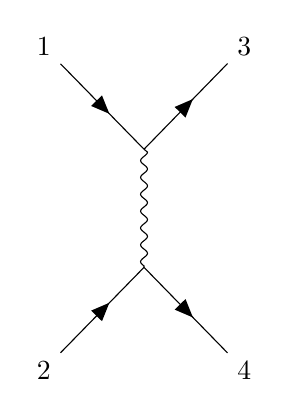
\begin{tikzpicture}
      \begin{feynman}
        \vertex (m1);
        \vertex [above left= of m1](i1) {1};
         \vertex [above right= of m1](f2) {3};
        \vertex [below= of m1](m3);
         \vertex [below left=of m3] (i2) {2};
        \vertex [below right=of m3] (f1) {4};
        \diagram*{
          (i1) -- [fermion] (m1),
          (m3) -- [photon] (m1) -- [fermion] (f2),
          (i2) -- [fermion] (m3),
          (m3) -- [fermion] (f1)
        };
      \end{feynman}
    \end{tikzpicture}
\end{center}
    \item `s-channel' (space-channel): represents the process in which particles 1 and 2 join into an intermediate particle that eventually splits into particles 3 and 4. It is the only way that resonances and new unstable particles may be discovered provided their lifetimes are long enough that they are directly detectable. The Mandelstam variable $s$ (also known as the centre-of-mass energy/invariant mass), involving the four-momenta, is
    $$s=(p_1+p_2)^2=(p_3+p_4)^2$$
    \begin{center}
    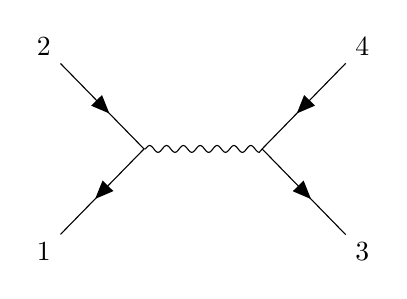
\begin{tikzpicture}
      \begin{feynman}
        \vertex (m1);
        \vertex [above left=of m1] (i1) {2};
        \vertex [below left=of m1] (i2) {1};
        \vertex [right=of m1] (m2);
        \vertex [above right=of m2] (f2) {4};
        \vertex [below right=of m2] (f1) {3};

        \diagram*{
          (i1) -- [fermion] (m1) -- [fermion] (i2),
          (f2) -- [fermion] (m2) -- [fermion] (f1),
          (m1) -- [photon] (m2)
        };
      \end{feynman}
    \end{tikzpicture}
\end{center}
    \item `u-channel': represents the `t-channel' where the role of the particles 3, 4 are interchanged. Used when the final states have identical particles and we cannot distinguish 3 and 4 (either t or u channel are equally valid). The Mandelstam variable $u$, involving the four-momenta, is
    $$u=(p_1-p_4)^2=(p_3-p_2)^2$$
       \begin{center}
    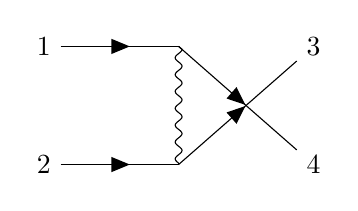
\begin{tikzpicture}
      \begin{feynman}
        \vertex (m1);
        \vertex [left= of m1](i1) {1};
         \vertex [right= of m1](f2) {3};
        \vertex [below= of m1](m3);
         \vertex [left=of m3] (i2) {2};
        \vertex [right=of m3] (f1) {4};
        \diagram*{
          (i1) -- [fermion] (m1),
          (m3) -- [photon] (m1) -- [fermion] (f1),
          (i2) -- [fermion] (m3),
          (m3) -- [fermion] (f2)
        };
      \end{feynman}
    \end{tikzpicture}
\end{center}
Note that this crossing is not a vertex.
\end{enumerate}

\end{eg}
\begin{remarks}\leavevmode
\begin{enumerate}
\item If all are particles (or anti-particles), only scattering diagrams are involved $a+b\rightarrow c+d$. Specifically, annihilation cannot occur. 
\item Remember to check symmetry (quantum statistics - bosons, fermions) for identical particles in the final state.
\end{enumerate}
\end{remarks}
\newpage
\section{QED and charged particles}
\subsection{Charged matter}
\begin{center}
\begin{tabular}{|c|c|c|}
\hline
Flavour     & Charged lepton mass & Neutral lepton mass \\
\hline
    e & $m_e=0.511$ MeV & $m_{\nu_e}\leq 10$ eV\\
    \hline
    $\mu$ & $m_\mu=105.66$ MeV & $m_{\nu_\mu}\leq 0.16$ MeV\\
    \hline
    $\tau$ & $m_\tau=1777$ MeV & $m_{\nu_\tau}\leq 18$ MeV\\
    \hline
\end{tabular}
\end{center}
\begin{eg}
Muon $\mu$ was discovered as a component of the cosmic radiation in 1937, and are decay products of short-lived mesons (integral-spin particles) produced in the upper atmosphere by primary cosmic ray protons from space. $\tau$ lepton was first observed in accelerator experiments in 1975. 
\end{eg}
Charged leptons undergo both electromagnetic and weak interactions. 
\begin{defi}[Lepton flavour number]
$L_e$, $L_\mu$, $L_\tau$ $+1$ for each lepton and $-1$ for each antilepton of the appropriate flavour. This must be conserved.
\end{defi}
\begin{eg}
$\mu^+\rightarrow e^++\nu_e+\overline{\nu}_\mu$ is allowed by conservation of lepton number, while $\mu^+\rightarrow e^++\gamma$ is forbidden (branching ratio of $\leq 10^{-9}$).
\end{eg}
Another class of charged particles are quarks. 
\begin{center}
\begin{tabular}{|c|c|c|}
\hline
Flavour     & Quantum number & Rest mass \\
\hline
    u or d & - & $m_u\approx m_d\approx 0.31$ GeV/c$^2$\\
    \hline
    s & $S=-1$ & $m_s\approx 0.50$ GeV/c$^2$\\
    \hline
    c & $C=+1$ & $m_{c}\approx 1.6$ GeV/c$^2$\\
    \hline
     b & $B=-1$ & $m_{b}\approx 4.6$ GeV/c$^2$\\
    \hline
     t & $T=+1$ & $m_{t}\approx 180$ GeV/c$^2$\\
    \hline
\end{tabular}
\end{center}
\begin{eg}
u and d quarks are found in protons and neutrons. s quark is discovered in the cosmic rays in the 1950s. The discovery of the c quark resulted from the observation of massive meson states of the type $c\overline{c}$ in 1974, and that of the b quark followed from the detection of even heavier mesons $b\overline{b}$ in 1977. Finally, the most massive quark, $t$, was observed in 1995.
\end{eg}
\begin{defi}[Quantum numbers]
In strong interactions between the quarks, the flavour quantum number is conserved. Quarks may change flavour (change $S$, $C$, etc) but only for a weak interaction.
\end{defi}
\begin{eg}
In a collision between hadrons containing u and d quarks only, it is possible to produce hadrons containing strange quarks, but only as a quark-antiquark $s\overline{s}$ pair.
\end{eg}
\subsection{QED}
\begin{defi}[QED]
Quantum electrodynamics (QED) is the gauge theory of electromagnetic interactions. The fields are described by the 4-potential $A^\mu$. The theory is invariant under a local guage transformation $\psi\rightarrow\psi'=e^{iq\alpha(\vec{r},t)}\psi$ with $A^\mu\rightarrow A^\mu+\partial^\mu\alpha$. The change in state of an electron $e^-$ requires a change in field. The interaction occurs via a virtual photon (photon propagator) $\gamma$ emission. Charge is conserved. 
\end{defi}
\begin{remarks}\leavevmode
\begin{enumerate}
\item The coupling constant at the EM vertex is proportional to the fermion charge $Qe\propto\sqrt{\alpha}$, where $\alpha=1/137$ is the fine structure constant (determines the spin-orbit splitting in atomic spectra). 
\item Energy, momentum, angular momentum, parity and charge are always conserved. The QED vertex never changes particle type or flavour.
\item In general, when there is a gauge symmetry, there will be a corresponding conserved charge, by Noether's theorem.
\end{enumerate}
\end{remarks}
\newpage
\begin{eg}[Important QED processes]\leavevmode
\begin{enumerate}
    \item Compton scattering $\gamma e^-\rightarrow\gamma e^-$ with cross-section $\sigma\propto e^4$.
    \item Bremsstrahlung $e^-\rightarrow e^-\gamma$ (involving nucleus $Ze$) with cross-section $\sigma\propto Z^2e^6$.
    \item Pair production $\gamma\rightarrow e^+e^-$ (involving nucleus $Ze$) with cross-section $\sigma\propto Z^2e^6$.
    \item Electron-positron annihilation $e^-e^+\rightarrow q\overline{q}$ with cross-section $\sigma\propto Q_q^2e^4$.
    \item Pion ($u\overline{u}$) decay $\pi^0\rightarrow\gamma\gamma$ with cross-section $\sigma\propto Q_u^4e^4$.
    \item $J/\psi$ ($c\overline{c}$)decay $J/\psi\rightarrow\mu^+\mu^-$ with cross-section $Q_c^2e^4$
\end{enumerate}
\end{eg}
\begin{remarks}
Consider the process of absorption (or emission) of a photon by an electron. The photon couples to the electron with amplitude $\sqrt{\alpha}$ and this process cannot occur for free particles, since an electron cannot absorb or emit a massless photon while conserving energy and momentum. The photoelectric effect of photon absorption by an electron involves momentum conservation by the whole atom. An electron cannot emit a real photon and conserve energy and momentum without reducing its rest mass (it is said to go `off mass shell).
\end{remarks}
\begin{eg}[Spinless $e$-$p$ scattering]
The matrix element is $\mathcal{M}=e^2/q^2=4\pi\alpha/q^2$. By Fermi's Golden Rule and Born's approximation
$$\frac{d\sigma}{d\Omega}=\frac{E^2}{(2\pi)^2}|\mathcal{M}|^2=\frac{4\alpha^2E^2}{q^4}$$
but the 4-momentum transfer (t-channel) is
$$t=q^2=(E_f-E_i)^2-(\vec{p}_f-\vec{p}_i)^2=2m_e^2-2E_iE_f+2|\vec{p}_f||\vec{p}_i|\cos\theta$$
  \begin{center}
    \begin{tikzpicture}
      \begin{feynman}
        \vertex (m1);
        \vertex [above=0.7 em of m1] {$e$};
        \vertex [above left= of m1](i1) {$e^-$};
         \vertex [below right= of m3](f1) {$p$};
        \vertex [below= of m1](m3);
        \vertex [below=0.7 em of m3] {$e$};
         \vertex [below left=of m3] (i2) {$p$};
        \vertex [above right=of m1] (f2) {$e^-$};
        \diagram*{
          (i1) -- [fermion] (m1),
          (m3) -- [photon, edge label = $\gamma/Z$] (m1) -- [fermion] (f2),
          (i2) -- [fermion] (m3),
          (m3) -- [fermion] (f1)
        };
      \end{feynman}
    \end{tikzpicture}
\end{center}
Neglecting electron's mass $m_e=0\implies|\vec{p}_f|=E_f$, we have $q^2=-2E_fE_i(1-\cos\theta)=-4E_fE_i\sin^2(\theta/2)$. For elastic scattering, $E_f=E_i=E$, so the cross-section is
$$\frac{d\sigma}{d\Omega}=\frac{\alpha^2}{4E^2\sin^4(\theta/2)}$$
Same result as that of Rutherford scattering.
\end{eg}
\begin{remarks}
The virtual $\gamma$ carries 4-momentum $q^\mu=(E,\vec{p})$. Large $q$ would mean large $\vec{p}$ (small $\lambda)$ and large $E$ (large $\omega$). High $q$ wavefunction oscillates rapidly in space and time, hence probing short distances and short time. We need large $q^2$ in order to probe internal structure, e.g. elastic scattering from the quarks in protons. Conversely, if $q^2$ is small, could only perform Rutherford scattering.
\end{remarks}
\begin{eg}[Spinless $e^+e^-$ scattering]
The cross-section is again $\frac{d\sigma}{d\Omega}=\frac{E^2}{(2\pi)^2}|\mathcal{M}|^2=\frac{4\alpha^2E^2}{q^4}$. The invariant mass (s-channel) is
$$s=q^2=(E_{e^+}+E_{e^-})^2-(\vec{p}_{e^+}+\vec{p}_{e^-})^2=(2E)^2$$
    \begin{center}
    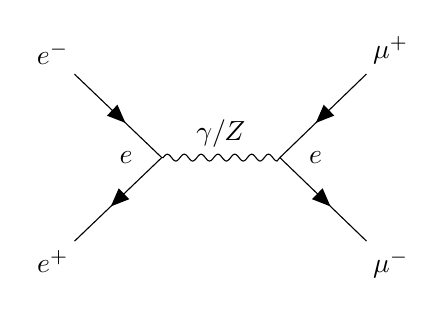
\begin{tikzpicture}
      \begin{feynman}
        \vertex (m1);
        \vertex [left=0.7 em of m1] {$e$};
        \vertex [above left=of m1] (i1) {$e^-$};
        \vertex [below left=of m1] (i2) {$e^+$};
        \vertex [right=of m1] (m2);
        \vertex [right=0.7 em of m2] {$e$};
        \vertex [above right=of m2] (f2) {$\mu^+$};
        \vertex [below right=of m2] (f1) {$\mu^-$};

        \diagram*{
          (i1) -- [fermion] (m1) -- [fermion] (i2),
          (f2) -- [fermion] (m2) -- [fermion] (f1),
          (m1) -- [photon, edge label = $\gamma/Z$] (m2)
        };
      \end{feynman}
    \end{tikzpicture}
\end{center}
Hence, the total cross-section is $\sigma=\int\frac{\alpha^2}{s}d\Omega=\frac{4\pi\alpha^2}{s}$.
\end{eg}
\begin{remarks}
When we use the Dirac equation, to factor in spin, the actual cross-section is
$$\frac{d\sigma}{d\Omega}=\frac{\alpha^2}{4s}(1+\cos^2\theta)\implies\sigma=\frac{4\pi\alpha^2}{3s}$$
\end{remarks}
\begin{eg}[Drell-Yan process]
The Drell–Yan process ($q\overline{q}\rightarrow l\overline{l}$) takes place when a quark of one hadron and an antiquark of another hadron annihilate, creating a virtual photon or Z boson which then decays into a pair of oppositely-charged leptons. Importantly, the energy of the colliding quark-antiquark pair can be almost entirely transformed into the mass of new particles. Take for instance, $\pi^-p\rightarrow\mu^+\mu^-$ and a bunch of hadrons.
\begin{center}
    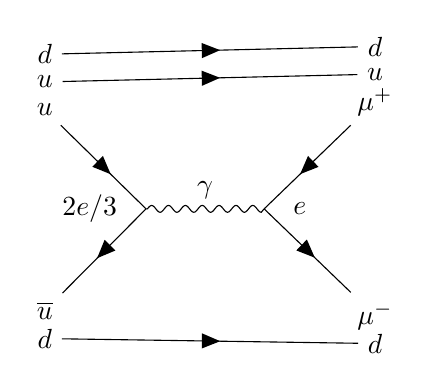
\begin{tikzpicture}
      \begin{feynman}
        \vertex (m1);
        \vertex [left=0.7em of m1] {$2e/3$};
        \vertex [above left=of m1] (i1) {$u$};
        \vertex [above=1 em of i1] (si2) {$u$};
        \vertex [above=1 em of si2] (si1) {$d$};
        \vertex [below left=of m1] (i2) {$\overline{u}$};
        \vertex [below= 1 em of i2] (si3) {$d$};
        \vertex [right=of m1] (m2);
        \vertex [right=0.7em of m2] {$e$};
        \vertex [above right=of m2] (f2) {$\mu^+$};
        \vertex [below right=of m2] (f1){$\mu^-$};
        \vertex [below=1 em of f1] (sf3) {$d$};
        \vertex [above= 1 em of f2] (sf2) {$u$};
        \vertex [above=1 em of sf2] (sf1) {$d$};
        \diagram*{
          (i1) -- [fermion] (m1) -- [fermion] (i2),
          (f2) -- [fermion] (m2) -- [fermion] (f1),
          (m1) -- [photon, edge label=$\gamma$] (m2),
          (si1) -- [fermion] (sf1),
          (si2) -- [fermion] (sf2),
          (si3) -- [fermion] (sf3)
        };
      \end{feynman}
    \end{tikzpicture}
\end{center}
The cross-section is $\sigma\propto Q_u^2e^4$. There are two $u$ quarks in the proton so the actual cross-section is twice of this.
\end{eg}
\begin{remarks}[Experimental tests of QED]
Higher order terms in QED introduce an anomalous magnetic moment, and thus for a point-like spin 1/2 particle, $g$ is not equal to 2 exactly, where $\vec{\mu}=g\frac{e}{2m}\vec{s}$. The theoretical anomaly is
$$\frac{g-2}{2}=0.5\frac{\alpha}{\pi}-0.32848\frac{\alpha^2}{\pi^2}+1.19\frac{\alpha^3}{\pi^3}+\dots=(115965230\pm10)\times10^{-11}$$
The agreement between theory and experiment [(115965219$\pm 1)\times10^{-11}$] is at the level of 1 in $10^8$.
\end{remarks}
\begin{remarks}[Running of $\alpha$]
$\alpha=\frac{e^2}{4\pi}$ specifies the strength of the interaction between an electron and a photon. $\alpha$ is not constant since the vacuum acts like a dielectric medium in the sense that quantum fluctuations can lead to a cloud of virtual $e^+e^-$ pairs. At large distances, the bare electron charge is screened. At shorter distances, the screening effect is reduced and we see a larger effective charge. Experimentally, we can measure $\alpha(q^2)$ from $e^+e^-\rightarrow\mu^+\mu^-$. $\alpha$ increases with increasing $q^2$
\end{remarks}
\begin{defi}[Vacuum polarization]
Due to the Coulomb field of the electrons, the vacuum containing the virtual $e^+e^-$ pair becomes polarized, and the effect is referred to as `vacuum polarization'.
\end{defi}
\newpage
\section{QCD}
\subsection{Quarks and gluons}
\begin{defi}[QCD]
Quantum chromodynamics is a gauge theory of the strong interaction, mediated by massless gluons (couples to `strong' charge) with interaction strength $\sqrt{\alpha_s}$ where $\alpha_s=\frac{g_s^2}{4\pi}\sim 1$. The symmetry for QCD is invariance under the local SU(3) transformation:
$$\psi\rightarrow\psi'=e^{ig\vec{\lambda}\cdot\vec{\Lambda}(\vec{r},t)}\psi$$
where $\lambda$ are eight $3\times 3$ matrices. The 8 massless gauge bosons (with spin-1) are called gluons, and thus mediate the strong force.
\end{defi}
\begin{remarks}
Only quarks have non-zero `strong' charge (colour) and therefore only quarks feel the strong interaction. QCD vertex never changes quark flavour and always conserves parity, energy, momentum, angular momentum and charge.
\end{remarks}
\begin{defi}[Colour]
Colour is a conserved quantum number with 3 values labelled red, green and blue. Quarks carry colour, while anti-quarks carry anti-colour. The SU(3) transformation operates on the colour state of the quark field. We may exchange colour but it is always conserved overall and at each vertex of the Feynman. At a three-point vertex, the gluon will carry away the difference in colour from the two quarks.
\end{defi}
\begin{eg}[Colourless particles]\leavevmode
\begin{enumerate}
    \item No colour at all: leptons, $\gamma$, W$^{\pm}$, $Z$
    \item Equal parts of all 3 colors $r$, $b$ and $g$: meson $q\overline{q}$ with $\frac{1}{\sqrt{3}}(r\overline{r}+b\overline{b}+g\overline{g})$ and baryon $qqq$ with $rgb$.
\end{enumerate}
\end{eg}
\begin{eg}[Gluons]
In contrast, gluons do not have equal parts of $r$, $b$ and $g$, so carry colour. As a result, gluons have self-couplings. The conventional 8 coloured orthogonal representations:
$$r\overline{b},~ r\overline{g}, ~g\overline{r},~g\overline{b},~b\overline{g},~b\overline{r},~\frac{1}{\sqrt{2}}(r\overline{r}-b\overline{b}),~\frac{1}{\sqrt{6}}(r\overline{r}+b\overline{b}-2g\overline{g})$$
The 9th orthogonal linear combination $\frac{1}{\sqrt{3}}(r\overline{r}+b\overline{b}+g\overline{g})$ is colourless.
\end{eg}
\begin{eg}[Gluon self-interaction]
For gluon-gluon scattering, we can have t-channel and s-channel, as well as, a 4-vertex interaction. We have same colour flow in each case, for instance, $r\overline{g}+g\overline{b}\rightarrow r\overline{r}+r\overline{b}$.
\end{eg}
\begin{defi}[QCD potential]
At short distances, the QCD potential has the Coulomb-like form $-C\alpha_s/r$ where $C$ is the colour factor, which is $C=4/3$ and $C=2/3$ for a colourless state in a meson and a baryon respectively. At large distances, the QCD potential has a linear form $kr$.
\end{defi}
\begin{remarks}
This colour factor $C$ arises from the fact that more gluon can participate in the process $q\rightarrow qg$. We obtain the colour factor from averaging over initial colour states and summing over final/intermediate colour states.
\end{remarks}
\begin{defi}[Confinement]
We never observe single free quarks or gluons. They are always confined within hadrons with an overall zero net colour charge, as a consequence of the strong interaction of gluons. Self-interaction of the gluons squeezes the lines of force into a narrow tube or string, with $V(r)\propto r$.
\end{defi}
\begin{defi}[Jets]
As quarks separate, the potential energy in the colour field increase linearly with separation. When the energy stored exceeds $2m_q$, new $q\overline{q}$ pairs are created. As energy decreases, hadrons (mainly mesons) freeze out. This process is called hadronisation. We start out with quarks and end up with narrow collimated jets of hadrons travelling in opposite directions.
\end{defi}
\begin{remarks}
The hadrons in a quark(antiquark) jet follow the direction of the original quark(antiquark). Hence, jets are produced in pairs and oriented back-to-back.
\end{remarks}
\begin{eg}[Nucleon-nucleon interactions]
Bound $qqq$ states are colourless (colour singlets). By conservation of colour charge, they can only emit and absorb another colour singlet state, i.e. not single gluons. They thus can only interact by the exchange of pions. The nuclear potential is a Yukawa potential $V(r)=-\frac{g^2}{4\pi}\frac{e^{-m_\pi r}}{r}$ with short range $1/m_\pi$ of about 1.4 fm.
\end{eg}
\begin{eg}[pp versus $\pi^+$p scattering]
QCD does not distinguish between quark flavours, only colour charge of quarks matters. At high energy (larger than the binding energy of quarks within hadrons), the ratio depends on the number of possible quark-quark combinations. Protons and $\pi^+$ have compositions $uud$ and $u\overline{d}$.
$$\frac{\sigma(\pi p)}{\sigma(pp)}=\frac{2\times 3}{3\times 3}$$
\end{eg}
\begin{remarks}[Running of $\alpha_s$]
In QCD, quantum fluctuations lead to a cloud of virtual $q\overline{q}$ pairs, which lead to `color screening'. The gluon self-interactions can also lead to a cloud of virtual gluons (which carries colour). The effect of quark polarization (drives $\alpha_s$ up at short distances) is opposite of that of gluon polarization (drives $\alpha_s$ down at short distances. The former depends on the number of quarks in the theory (number of flavours $f$) whereas the latter depends on the number of gluons (number of colours, $c$), the critical parameter is $2f-11n$. In the Standard Model, $a=2(6)-11(3)=-21$.\\[5pt]
Hence, the effective colour charge decreases at smaller distances (high energy). At low energies, $\alpha_s$ is thus large and we cannot use perturbation theory. Conversely, (opposite effect as QED) at high energies, $\alpha_s$ is small and we can treat quarks as free particles, i.e. asymptotic freedom.
\end{remarks}
\begin{eg}[OZI rule]
The $\phi$ (s$\overline{s}$) meson decays much more often into two $K$'s than into three $\pi$'s despite three pion decay being energetically favoured. The three-pion diagram can be cut in two by snipping only gluon lines. OZI rule states that such processes are `suppressed', but not absolutely forbidden. The OZI rule is related to asymptotic freedom. In an OZI-suppressed diagram, the gluons must be `hard' (high energy) since they carry the energy necessary to make the hadrons into which they fragment. But asymptotic freedom says that gluons couple weakly at high energies (short ranges). By contrast, in OZI-allowed processes, the gluons are `soft' (low energy) and the coupling is strong.
\end{eg}
\subsection{Experimental tests}
\subsubsection{Evidence for Color}
\begin{eg}[$e^+e^-$ annihilation at high energies]
Compare the cross-sections for $e^+e^-\rightarrow\mu^+\mu^-$ and $e^+e^-\rightarrow q\overline{q}$. The matrix elements are
$$\mathcal{M}(e^+e^-\rightarrow\mu^+\mu^-)\sim\frac{\alpha}{q^2},\quad\mathcal{M}(e^+e^-\rightarrow q\overline{q})\sim\frac{\alpha Q_q}{q^2}$$
If we neglect the mass of the final state quarks/muons, then the only difference is the charge of the final state particles. When measuring $\sigma(e^+e^-\rightarrow$hadrons), we not just measure a single quark of a given colour. The jet from the $u$-quark looks just like a jet from a $d$-quark, etc. We thus need to sum over all available flavours (which are kinematically accessible at a given centre-of-mass energy $\sqrt{s}$) and colours:
$$R=\frac{\sigma(e^+e^-\rightarrow\text{hadrons})}{\sigma(e^+e^-\rightarrow\mu^+\mu^-)}=3\sum_{i\in\text{allowed}}Q_i^2$$
As energy is increased, we expect to see steps in $R$:
\begin{center}
\begin{tabular}{|l|l|}
\hline
Energy & Expected ratio $R$     \\
\hline
$\sqrt{s}>2m_s\sim$ 1GeV    & uds: $3((2/3)^2+(1/3)^2+(1/3)^2)=2$     \\
\hline
$\sqrt{s}>2m_c\sim$ 4GeV    & udsc: $3((2/3)^2+(1/3)^2+(1/3)^2+(2/3)^2)=3+\frac{1}{3}$     \\
\hline
$\sqrt{s}>2m_b\sim$ 10GeV    & udscb: $3((2/3)^2+(1/3)^2+(1/3)^2+(2/3)^2+(1/3)^2)=3+\frac{2}{3}$     \\
\hline
$\sqrt{s}>2m_t\sim$ 350GeV    & udscbt: $3((2/3)^2+(1/3)^2+(1/3)^2+(2/3)^2+(1/3)^2+(2/3)^2)=5$     \\
\hline
\end{tabular}
\end{center}
We further observe bound state resonances (charmonium and bottomonium) for $\sqrt{s}<11$ GeV and low edge of Z resonance ($\Gamma\sim 2.5$ GeV) for $\sqrt{s}>50$ GeV.
\end{eg}
\begin{eg}[Existence of $\Omega^-$ (sss)]
$\Omega^-$ is a $L=0$ spin-3/2 baryon consisting of three $s$-quarks. Consider the wavefunction (spin and flavour)
$$\psi=|s\rangle|\uparrow\rangle|s\rangle|\uparrow\rangle|s\rangle|\uparrow\rangle$$
which is symmetric under particle interchange. But, quarks are fermions and have an overall anti-symmetric wavefunction, hence there exists a colour wavefunction which is anti-symmetric
$$\psi_{\text{color}}=\frac{1}{\sqrt{6}}(rgb+gbr+brg-grb-rbg-bgr)$$
There is a need to introduce a new quantum number to distinguish the three quarks to avoid violation of the Pauli's Exclusion Principle.
\end{eg}
\begin{eg}[Drell-Yan process]
Consider the conversion of the quarks $u\overline{u}\rightarrow\mu^+\mu^-$ in the reaction $\pi^-p$. We require to specify the colour of the annihilation quark, which must match, to form a virtual photon. The cross-section also has an additional suppression factor that is only accounted for if there is colour.
\end{eg}
\subsubsection{Evidence for Gluons}
\begin{eg}[$e^-e^+\rightarrow q\overline{q}g$]
Quarks can radiate gluons. The matrix element has an additional factor of $\sqrt{\alpha_s}$. 
\end{eg}
\begin{eg}[Jets]
Experimentally, we detect gluons as an additional jet: 3-jet events. The angular distribution of gluon jet depends on the gluon spin. Specifically, the distribution of the angle $\phi$ between the highest energy jet relative to the flight direction of the other two, in the centre of momentum frame, gives the spin of the gluon.\\[5pt]
Direct evidence for gluon self-interactions comes from 4-jet events. The angular distribution of the jets is sensitive to existence of triple gluon vertex (which consits of three spin-1 gluons). In contrast, the $qqg$ vertex only consists of two spin-$1/2$ quarks and one spin-1 gluon. Define the two lowest energy jets as the gluons (since they are more likely to be lower than quark jets). Measure the angle $\chi$ between the plane containing the quark jets and the plane containing the gluon jets.
\end{eg}
\begin{remarks}
The angular distribution of the two hadron jets is proof of spin 1/2 for the pointlike constituents of hadrons.
\end{remarks}
\subsubsection{Measurement of $\alpha_s$}
\begin{eg}[$e^+e^-$ annihilation]
In the continuum, the ratio $R=\sigma(e^+e^-\rightarrow \text{hadrons})$ includes an additional factor:
$$R=3\sum Q_q^2\bigg(1+\frac{\alpha_s}{\pi}\bigg)$$
For example, an $r\overline{r}$ colour state of $q\overline{q}$ can also arise from a $g\overline{g}$ state which has undergone $\overline{r}g$ gluon exchange with probability of order $\alpha_s$.
\end{eg}
\begin{eg}[3-jet rate $e^+e^-\rightarrow q\overline{q}g$]
Compare event shapes in $e^+e^-$ annihilation to hadrons, i.e. three-jet to two-jet events:
$$R_3=\frac{\sigma(e^+e^-\rightarrow 3j)}{\sigma(e^+e^-\rightarrow 2j)}\propto\alpha_s$$
which was measured to decrease with energy, as expected.
\end{eg}
\begin{eg}
The decay mode $\Sigma^0\rightarrow\Lambda\gamma$ involves no change in quark flavour. $\Lambda$ has spin $1/2$ and is also a uds combination, but it is a charge singlet state, and strong decay is forbidden (due to conservation of isospin). This decay proceeds by an electromagnetic transition with a lifetime of $10^{-19}$ s. By contrast, $\Sigma^0\rightarrow\Lambda\pi^0$ is a strong, isospin-conserving decay. It is a broad state with width $\Gamma=36$ MeV and a calculated lifetime $\tau=\hbar/\Gamma=10^{-23}$ s. Disregarding the factor 3 differences in the total kinetic energy liberated in the two cases, and with the decay rate for a leading-order process proportional to the square of the coupling constant, we estimate that the strong coupling $\alpha_s$ to be
$$\frac{\alpha_s}{\alpha}\sim\sqrt{\frac{10^{-19}}{10^{-23}}}\sim 100$$
\end{eg}
\newpage
\section{Quark model of hadrons}
\begin{remarks}[Evidence for quarks]\leavevmode
\begin{enumerate}
    \item The magnetic moments of proton and neutron are not just $\mu_N=\frac{e\hbar}{2m_p}$ and 0 respectively.
    \item Electron-proton scattering at high $q^2$ deviates from Rutherford scattering.
    \item Hadron jets are observed in $e^+e^-$ and $pp$ collisions.
    \item Symmetries (patterns) in masses and properties of hadron states, `quarky' periodic table.
    \item Steps in $R$.
    \item Observation of $c\overline{c}$ and $b\overline{b}$ bound states.
\end{enumerate}
All of these examples, out of many more, suggests hadrons have internal structure.
\end{remarks}
\subsection{Light quarks}
\begin{defi}[Hadron wavefunctions]
We treat quarks as identical fermions with states labelled with spatial, spin, flavour and colour. All hadrons are colour singlets (net colour zero). 
$$\psi_{\text{color}}^{q\overline{q}}=\frac{1}{\sqrt{3}}(r\overline{r}+g\overline{g}+b\overline{b})$$
$$\psi_{\text{color}}^{qqq}=\frac{1}{\sqrt{6}}(rgb+gbr+brg-grb-rbg-bgr)$$
\end{defi}
\begin{defi}[Parity]
The parity operator $\hat{P}$ performs spatial inversion $\vec{r}\rightarrow-\vec{r}$. The eigenvalue of $\hat{P}$ is called parity $P=\pm1$. Most particles are eigenstates of parity and $P$ represents the particle's internal parity.
\end{defi}
\begin{remarks}\leavevmode
\begin{enumerate}
\item If the Hamiltonian for an interaction commutes with $\hat{P}$, then $[\hat{P},\hat{H}]=0$, i.e. conserved in the interaction. Parity is conserved in the strong and the EM interactions, but not in the weak interaction.
\item The composite system of two particles with orbital angular momentum $L$ has parity $P=P_1P_2(-1)^L$, where $P_{1,2}$ are intrinsic parities of particles 1 and 2. Mesons $q\overline{q}$ have overall parity of $-1$.
\item Quantum field theory tells us that fermions and anti-fermions have opposite parity, while bosons and antibosons have the same parity. For quarks and leptons, we choose $P_{q,l}=+1$ and $P_{\overline{q},\overline{l}}=-1$. For gauge bosons, they have $P=-1$.
\end{enumerate}
\end{remarks}
\begin{notation}
$J^P$ represents the angular momentum $J$ and the parity $P$.
\end{notation}
\begin{eg}
Parity is conserved in strong and electromagnetic interactions.
\begin{itemize}
    \item $p+p\rightarrow\pi^++p+n$. Necessary to assign an intrinsic parity to the pion in order to ensure the same parity in initial and final states, $P_\pi=-1$. By convention, neutrons and protons are assigned the same $P_n=+1$.
    \item $p+p\rightarrow K^++\Lambda+p$. Only the parity of the $\Lambda K$ pair, relative to the nucleon, can be measured, and it is found to be odd. By convention, the hyperon $\Lambda$ is assigned the same (even) parity as the nucleon, so that of the kaon $K^+$ is odd.
\end{itemize}
\end{eg}
\subsection{Light mesons}
\begin{eg}
Consider ground state ($L=0$) mesons, consisting of light quarks ($u$, $d$, $s$) with masses $m_u\sim 0.3 GeV$, $m_d\sim 0.3 GeV$, $m_s\sim 0.5 GeV$. The masses (MeV) of some light mesons examples:
$$\pi(140),~K(495),~\eta(550),~\eta'(960),~\rho(770),~K^*(890),~\omega(780),~\phi(1020)$$
\end{eg}
\begin{defi}[Pseudoscalar and vector mesons]
There are two possible $q\overline{q}$ total spin states (since each $q$ has $s=1/2$), we have $S=0$ (pseudoscalar mesons) and $S=1$ (vector mesons). There are 9 each, forming a nonet.
\end{defi}
\begin{defi}[Isospin and strangeness]
To understand the quark structure of matter, two quantum numbers were introduced: isospin and strangeness
$$I=\frac{1}{2}(n_u-n_d-n_{\overline{u}}+n_{\overline{d}}),\quad S=-(n_s-n_{\overline{s}})$$
where $n$ is the number of quarks.
\end{defi}
\begin{notation}[Quark multiplet]
To represent the quark multiplets, we plot the quantum numbers (strangeness against isospin).
\end{notation}
\begin{figure}[H]
    \centering
    \includegraphics[width=\linewidth]{multiplet1.JPG}
\end{figure}
\begin{defi}[Eightfold way]
Murray Gell-Mann arranged the baryons and mesons into weird geometrical patterns according to their charge and strangeness. Particles of like charge lie along the downward sloping diagonal lines. Horizontal and vertical lines associate particles of like strangeness and isospin respectively.
\end{defi}
\begin{defi}[Meson nonet]
The nine lightest mesons (which are pseudoscalars) fill a hexagonal pattern called meson nonet. The nine heavier mesons (which are vectors) fill a hexagonal pattern as well.
\end{defi}
\begin{figure}[H]
    \centering
    \includegraphics[width=\linewidth]{multiplet2.JPG}
\end{figure}
\begin{eg}
The states $u\overline{u}$, $d\overline{d}$ and $s\overline{s}$ all have zero flavour quantum numbers and can mix.
$$J^P=0^-:\quad\pi^0=\frac{1}{\sqrt{2}}(u\overline{u}-d\overline{d}),~\eta=\frac{1}{\sqrt{6}}(u\overline{u}+d\overline{d}-2s\overline{s}),~\eta'=\frac{1}{\sqrt{3}}(u\overline{u}+d\overline{d}+s\overline{s})$$
$$J^P=1^-:\quad\rho^0=\frac{1}{\sqrt{2}}(u\overline{u}-d\overline{d}),~\omega^0=\frac{1}{\sqrt{2}}(u\overline{u}+d\overline{d}),~\phi=s\overline{s}$$
where the mixing coefficients are determined experimentally from meson masses and decays.
\end{eg}
\begin{remarks}[Isospin sets]
The pion triplet has $I=1$ and consists of $\pi^+$, $\pi^0$ and $\pi^-$ with isospin $I_z=+1$, 0 and $-1$ respectively. The Kaon doublet (two copies) has $I=1/2$ and consists of $K^{+,0}$, $K^{0,-}$ with $I_z=\pm1/2$ each. The Eta has two copies of singlets with $I=0$, i.e. $\eta$ and $\eta'$ has $I_z=0$.
\end{remarks}

\begin{eg}[Leptonic decays of vector mesons]
Consider the decay $\rho^0\rightarrow e^+e^-$. The width is
$$\mathcal{M}\sim\frac{e}{q^2}\bigg[\frac{1}{\sqrt{2}}(Q_ue-Q_de)\bigg]\implies\Gamma(\rho^0\rightarrow e^+e^-)\propto\bigg[\frac{1}{\sqrt{2}}\bigg(\frac{2}{3}-\frac{-1}{3}\bigg)\bigg]^2=\frac{1}{2}$$
Similarly, for $\omega^0$ and $\phi$, we have $\frac{1}{18}$ and $\frac{1}{9}$, giving an overall ratio of partial widths $\Gamma_{\rho^0}$, $\Gamma_{\omega^0}$ and $\Gamma_\phi$ to be 9 to 1 to 2.
\end{eg}
\begin{prop}
Spin-spin interaction, between the quark and the anti-quark, contributes to the masses of mesons. The relation is
$$M_{q\overline{q}}=m_q+m_{\overline{q}}+\frac{A}{m_qm_{\overline{q}}}\bigg(\frac{1}{2}S^2-\frac{3}{4}\bigg)$$
where $S^2=0$ and $S^2=1(1+1)=2$ for $J^P=0^-$ and $1^-$ mesons ($L=0$) respectively.
\end{prop}
\begin{proof}
For a state of spin $\vec{S}=\vec{S}_1+\vec{S}_2$, we have
$$\vec{S}_1\cdot\vec{S}_2=\frac{1}{2}(\vec{S}^2-\vec{S}_1^2-\vec{S}_2^2)=\frac{1}{2}\vec{S}^2-\frac{3}{4}$$
where $\vec{S}_1^2=\vec{S}_2^2=\frac{3}{4}$.
\end{proof}
\begin{remarks}
This color magnetic interaction is akin the the hyperfine splitting in QED. $A$ is determined experimentally. 
\end{remarks}
\begin{eg}
For $\eta=\frac{1}{\sqrt{6}}(u\overline{u}+d\overline{d}-2s\overline{s})$, the mass is
$$M_\eta=\frac{1}{6}\bigg(2m_u-\frac{3A}{4m_u^2}\bigg)+\frac{1}{6}\bigg(2m_d-\frac{3A}{4m_d^2}\bigg)+\frac{4}{6}\bigg(2m_s-\frac{3A}{4m_s^2}\bigg)$$
\end{eg}
\subsection{Light baryons}
Baryons are made of three indistinguishable quarks.
\begin{prop}
For baryon ground states, $\psi_{\text{spin}}\psi_{\text{flavour}}$ must be symmetric.
\end{prop}
\begin{proof}
As baryons are fermions, the overall wavefunction must be anti-symmetric under the interchange of any two quarks. For baryon ground states, $L=0$ and hence $\psi_{\text{space}}$ is symmetric. All hadrons are colour singlets (colourless), then the colour wavefunction is anti-symmetric
$$\psi_{\text{colour}}=\frac{1}{\sqrt{6}}(rgb+gbr+brg-grb-rbg-bgr)$$
Hence, the product of the remaining two wavefunctions must be symmetric.
\end{proof}
\begin{remarks}
By abuse of notation, we do not include the ket notation for the following. Instead of using $|0.5,\pm0.5\rangle$ for the individual spins, we use the intuitive notation $\uparrow$, $\downarrow$.
\end{remarks}
\begin{cor}[Three-quark spin wavefunction]
The $J=\frac{3}{2}$ spin wavefunctions are symmetric under the interchange of any two quarks, and the possible wavefunctions are
$$|1.5,1.5\rangle_{q_1q_2q_3}=\uparrow\uparrow\uparrow,\quad|1.5,0.5\rangle_{q_1q_2q_3}=\frac{1}{\sqrt{3}}(\downarrow\uparrow\uparrow+\uparrow\downarrow\uparrow+\uparrow\uparrow\downarrow)$$
$$|1.5,-0.5\rangle_{q_1q_2q_3}=\frac{1}{\sqrt{3}}(\uparrow\downarrow\downarrow+\downarrow\uparrow\downarrow+\downarrow\downarrow\uparrow),\quad|1.5,-1.5\rangle_{q_1q_2q_3}=\downarrow\downarrow\downarrow$$
The $J=\frac{1}{2}$ spin wavefunctions can either be
$$|0.5,0.5\rangle_{q_1q_2q_3}=\frac{1}{\sqrt{2}}(\uparrow\downarrow\uparrow-\downarrow\uparrow\uparrow),\quad|0.5,-0.5\rangle_{q_1q_2q_3}=\frac{1}{\sqrt{2}}(\uparrow\downarrow\downarrow-\downarrow\uparrow\downarrow)$$
which is anti-symmetric under the interchange of the first two quarks (ordering matters) or
$$|0.5,0.5\rangle_{q_1q_2q_3}=\frac{1}{\sqrt{6}}(2\downarrow\downarrow\uparrow-\downarrow\uparrow\downarrow-\uparrow\downarrow\downarrow),\quad|0.5,-0.5\rangle_{q_1q_2q_3}=\frac{1}{\sqrt{6}}(2\downarrow\downarrow\uparrow-\downarrow\uparrow\downarrow-\uparrow\downarrow\downarrow)$$
which is symmetric under the interchange of the first two quarks (ordering matters)
\end{cor}
\begin{proof}
With three spin-1/2 quarks, the total spin is $J=\frac{1}{2}\oplus\frac{1}{2}\oplus\frac{1}{2}$ which is 0.5 or 1.5.
\begin{itemize}
    \item $J=1/5$: Trivially, we can write down the state $|1.5,1.5\rangle_{q_1q_2q_3}$, where the spins are all pointed upwards. Apply $\hat{J}_-$:
    \begin{align}
        \hat{J}_-|1.5,1.5\rangle_{q_1q_2q_3}&=(\hat{J}_-\uparrow)\uparrow\uparrow+\uparrow(\hat{J}_-\uparrow)\uparrow+\uparrow\uparrow(\hat{J}_-\uparrow)\nonumber\\\sqrt{\frac{3}{2}\frac{5}{2}-\frac{3}{2}\frac{1}{2}}|1.5,0.5\rangle_{q_1q_2q_3}&=\downarrow\uparrow\uparrow+\uparrow\downarrow\uparrow+\uparrow\uparrow\downarrow\nonumber\\|1.5,0.5\rangle_{q_1q_2q_3}&=\frac{1}{\sqrt{3}}(\downarrow\uparrow\uparrow+\uparrow\downarrow\uparrow+\uparrow\uparrow\downarrow)\nonumber
    \end{align}
    Similarly, write down the state $|1.5,-1.5\rangle_{q_1q_2q_3}$. Apply $\hat{J}_+$:
    \begin{align}
        \hat{J}_+|1.5,-1.5\rangle_{q_1q_2q_3}&=(\hat{J}_+\downarrow)\downarrow\downarrow+\downarrow(\hat{J}_+\downarrow)\downarrow+\downarrow\downarrow(\hat{J}_+\downarrow)\nonumber\\\sqrt{\frac{3}{2}\frac{5}{2}+\frac{3}{2}\frac{1}{2}}|1.5,-0.5\rangle_{q_1q_2q_3}&=\uparrow\downarrow\downarrow+\downarrow\uparrow\downarrow+\downarrow\downarrow\uparrow\nonumber\\|1.5,0.5\rangle_{q_1q_2q_3}&=\frac{1}{\sqrt{3}}(\uparrow\downarrow\downarrow+\downarrow\uparrow\downarrow+\downarrow\downarrow\uparrow)\nonumber
    \end{align}
\item $J=0.5$: For $J=0.5$, we can either have $|0.5,0.5\rangle_{q_1q_2q_3}$ or $|0.5,-0.5\rangle_{q_1q_2q_3}$.
\begin{itemize}
    \item First consider the case where the first two quarks $q_1q_2$ are in an overall spin anti-symmetric state $|0,0\rangle_{q_1q_2}=\frac{1}{\sqrt{2}}(\uparrow\downarrow-\downarrow\uparrow)$. To have an overall $J=1/2$, we require the third quark to be in the $J=1/2$ state $\implies m_{j,q_3}=\pm\frac{1}{2}$ depending on $m_J$. Hence,
    $$|0.5,0.5\rangle_{q_1q_2q_3}=\frac{1}{\sqrt{2}}(\uparrow\downarrow\uparrow-\downarrow\uparrow\uparrow),\quad|0.5,-0.5\rangle_{q_1q_2q_3}=\frac{1}{\sqrt{2}}(\uparrow\downarrow\downarrow-\downarrow\uparrow\downarrow)$$
    \item Second consider the case where the first two quarks are in an overall spin symmetric state, which can be $|1,1\rangle_{q_1q_2}=\uparrow\uparrow$ and $|1,0\rangle_{q_1q_2}=\frac{1}{\sqrt{2}}(\uparrow\downarrow+\downarrow\uparrow)$. For a $|0.5,0.5\rangle_{q_1q_2q_3}$ baryon, there are two possible combinations. If $|q_1,q_2\rangle=\uparrow\uparrow$, then the third quark has $m_{j,q_3}=-0.5$. If $|q_1,q_2\rangle=\frac{1}{\sqrt{2}}(\uparrow\downarrow+\downarrow\uparrow)$, then the third quark has $m_{j,q_3}=+0.5$. Take linear combination.
    $$|0.5,0.5\rangle_{q_1q_2q_3}=c_1|1,1\rangle_{q_1q_2}|0.5,-0.5\rangle_{q_3}+c_2|1,0\rangle_{q_1q_2}|0.5,0.5\rangle_{q_3}$$
    Take $J_+$ on both sides
    \begin{eqnarray}
        0&=&J_+|0.5,0.5\rangle_{q_1q_2q_3}\nonumber\\&=&c_1\bigg[(J_+|1,1\rangle)_{q_1q_2}|0.5,-0.5\rangle_{q_3}+|1,1\rangle_{q_1q_2}(J_+|0.5,-0.5\rangle_{q_3})\bigg]\nonumber\\&&+c_2\bigg[(J_+|1,0\rangle_{q_1q_2})|0.5,0.5\rangle_{q_3}+|1,0\rangle_{q_1q_2}(J_+|0.5,0.5\rangle_{q_3})\bigg]\nonumber\\&=&c_1\bigg[0+|1,1\rangle_{q_1q_2}|0.5,0.5\rangle_{q_3}\bigg]+c_2\bigg[\sqrt{2}|1,1\rangle_{q_1q_2}|0.5,0.5\rangle_{q_3}+0\bigg]\implies c_1=-\sqrt{2}c_2\nonumber
    \end{eqnarray}
    But, by normalization, we require $c_1^2+c_2^2=1$. Hence, $c_1=\sqrt{2/3}$ and $c_2=-\sqrt{1/3}$. By a similar procedure, we can obtain $|0.5,-0.5\rangle_{q_1q_2q_3}$.
\end{itemize}
\end{itemize}
\end{proof}
\begin{prop}
The Quark Model predicts that light baryons appear in decuplets (10 of them) of spin $3/2$ states and octets (8 of them) of spin $1/2$ states.
\end{prop}
\begin{proof}\leavevmode
\begin{enumerate}
    \item case: quarks are all the same flavour (uuu, ddd, sss) $\implies\psi_{\text{flavour}}$ is symmetric under the interchange of any two quarks. Since $\psi_{\text{spin}}\psi_{\text{flavour}}$ is symmetric, we require $\psi_{\text{spin}}$ to be symmetric under the interchange of any two quarks. This is only satisfied by the $J=3/2$ states (three of them).
    \item case: two quarks have the same flavour (uud, uus, ddu, dds, ssu, ssd) $\implies\psi_{\text{flavour}}$ is symmetric for the interchange of the two $q_1q_2$.  Since $\psi_{\text{spin}}\psi_{\text{flavour}}$ is symmetric, we require $\psi_{\text{spin}}$ to be symmetric under $q_1\leftrightarrow q_2$. This is satisfied by the $J=3/2$ and $J=1/2$ states (there are 6 of them each).
    \item case: quarks are all different flavours $uds$
    \begin{itemize}
        \item the flavour $ud$ is symmetric, i.e. $\frac{1}{\sqrt{2}}(ud+du)$. Again, require $\psi_{\text{spin}}$ to be symmetric under the interchange of $ud$. This is satisfied by the $J=3/2$ and $J=1/2$ states, so there is one $J=3/2$ and one $J=1/2$ state (uds);
        \item the flavour $ud$ is anti-symmetric, i.e. $\frac{1}{\sqrt{2}}(ud-du)$. Again, require $\psi_{\text{spin}}$ to be anti-symmetric under the interchange of $ud$. This is only satisfied by the $J=1/2$ states, so there is one $J=1/2$ state (uds).
    \end{itemize}
\end{enumerate}
Thus, in total there are 10 spin $3/2$ states and 8 spin $1/2$ states.
\end{proof}
\begin{figure}[H]
    \centering
    \includegraphics[width=\linewidth]{multiplet3.JPG}
\end{figure}
\begin{defi}[Baryon octet and decuplet]
The 8 lightest baryons fit into a hexagonal array, known as the baryon octet. The 10 heavier baryons fit into a triangular array, known as the baryon decuplet. 
\end{defi}
\begin{remarks}\leavevmode
\begin{enumerate}
\item There are no $J=1/2$ uuu, ddd, sss baryons with $L=0$.
\item Antibaryons are in separate multiplets (not shown). For example, the anti-particle of $\Sigma^+$ (uus) is $\overline{\Sigma}^-$ ($\overline{u}\overline{u}\overline{s}$) with $J^P=\frac{1}{2}^-$ and not $\Sigma^-$ (dds) with $J^P=\frac{1}{2}^+$.
\end{enumerate}
\end{remarks}
\begin{prop}[Baryon mass]
$$M_{qqq}=m_1m_2+m_3+A'\bigg(\frac{\vec{S}_1}{m_1}\cdot\frac{\vec{S}_2}{m_2}+\frac{\vec{S}_1}{m_1}\cdot\frac{\vec{S}_3}{m32}+\frac{\vec{S}_2}{m_2}\cdot\frac{\vec{S}_3}{m_3}\bigg)$$
\end{prop}
\begin{eg}
Suppose all quarks have the same mass, then $M_{qqq}=3m_q+A'\sum_{i<j}\frac{\vec{S}_i\cdot\vec{S}_j}{m_q^2}$. For a system of three spins,
$$\vec{S}^2=(\vec{S}_1+\vec{S}_2+\vec{S}_3)^2=\vec{S}_1^2+\vec{S}_2^2+\vec{S}_3^2+2\sum_{i<j}\vec{S}_i\cdot\vec{S}_j=\sum_{i=1,2,3}\vec{S}_i^2+S(S+1)-3\frac{1}{2}\bigg(\frac{1}{2}+1\bigg)$$
The last term gives $S(S+1)-9/4$, which is $-3/2$ and $3/2$ for $J=1/2$ and $J=3/2$ respectively. Proton and $\Delta$ has the same quark content $uud$. Their masses are, however, different:
$$M_p=3m_u-\frac{3A'}{4m_u^2},\quad M_\Delta=3m_u+\frac{3A'}{4m_u^2}$$
\end{eg}
\begin{remarks}
The constituent quark mass depends on the hadron wavefunction, and includes cloud of gluons and $qq$ pairs, i.e. slightly different values for mesons and baryons.
\end{remarks}
\begin{defi}[Magnetic dipole moment]
Magnetic dipole moment is the maximum measureable component of the magnetic dipole moment operator. Magnetic dipole moments arise from the orbital motion of charged quarks and the intrinsic spin-related magnetic moments of the quarks.
$$\mu_\ell=\langle\psi_{\text{space}}|g_\ell\frac{q}{2m}\hat{L}_z|\psi_{\text{space}}\rangle=-\frac{g_\ell e\hbar\ell}{2m_e}=-\mu_B\ell,\quad\mu_s=\langle\psi_{\text{spin}}|\frac{g_sq}{2m}\hat{S}_z|\psi_{\text{spin}}\rangle=-\frac{g_se}{2m_e}\frac{\hbar}{2}=-\mu_B$$
where $\mu_B=e\hbar/2m_e$ is the Bohr magneton. Similarly, we can define the nuclear magneton $\mu_N=\frac{e\hbar}{2m_p}$.
\end{defi}
\begin{prop}[Baryon magnetic moments]
For quarks bound within an $\ell=0$ baryon:
$$\mu_{\text{baryon}}=\bigg\langle\psi_{\text{spin}}^B\bigg|\frac{q_1}{m_1}\hat{S}_{1z}+\frac{q_2}{m_2}\hat{S}_{2z}+\frac{q_1}{m_3}\hat{S}_{3z}\bigg|\psi_{\text{spin}}^B\bigg\rangle$$
\end{prop}
\begin{eg}[Proton]
Consider a spin up proton with $J=0.5$. The wavefunction is
$$|\psi_{\text{spin}}\rangle=\frac{1}{\sqrt{6}}(2|\uparrow\rangle_{u}|\uparrow\rangle_{u}|\downarrow\rangle_{d}-|\uparrow\rangle_{u}|\downarrow\rangle_{u}|\uparrow\rangle_{d}-|\downarrow\rangle_{u}|\uparrow\rangle_{u}|\uparrow\rangle_{d})$$
The magnetic moment is
\begin{align}
\mu^p&=\frac{1}{6}\langle 2\uparrow\uparrow\downarrow-\uparrow\downarrow\uparrow-\downarrow\uparrow\uparrow|\hat{\mu}_1+\hat{\mu}_2+\hat{\mu}_3|2\uparrow\uparrow\downarrow-\uparrow\downarrow\uparrow-\downarrow\uparrow\uparrow\rangle\nonumber\\&=\frac{1}{6}\langle 2\uparrow\uparrow\downarrow|\sum_{i=1,2,3}\hat{\mu}_i|2\uparrow\uparrow\downarrow\rangle+\frac{1}{6}\langle -\uparrow\downarrow\uparrow|\sum_{i=1,2,3}\hat{\mu}_i|-\uparrow\downarrow\uparrow\rangle+\frac{1}{6}\langle -\downarrow\uparrow\uparrow|\sum_{i=1,2,3}\hat{\mu}_i|-\downarrow\uparrow\uparrow\rangle\nonumber\\&=\frac{1}{6}[4(\mu_1+\mu_2)-2\mu_3]\nonumber
\end{align}
We assume $m_u=m_d$ and $\mu_1=\mu_2=\mu_u$, $\mu_3=\mu_d=-0.5\mu_u$, hence $\mu^p=\frac{4}{3}\mu_u-\frac{1}{3}\mu_d=\frac{3}{2}\mu_u=\frac{e\hbar}{2m_u}=\frac{m_p}{m_u}\mu_N$. Do the same for neutrons and we can show $\mu_n/\mu_p=-2/3$.
\end{eg}
\newpage
\subsection{Hadron decays}
Hadrons are eigenstates of the strong force and will decay via the strong interaction to lighter mass states if energetically feasible. Angular momentum and parity must be conserved in strong decays.
\begin{eg}[$\rho^0\rightarrow\pi^+\pi^-$]
Take $\rho^0$ to be $u\overline{u}$. $\pi^+$ and $\pi^-$ will be $u\overline{d}$ and $\overline{d}u$ respectively.
\begin{center}
    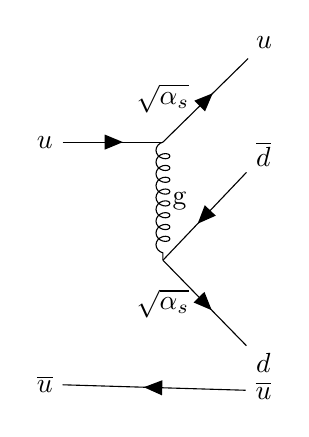
\begin{tikzpicture}
      \begin{feynman}
        \vertex (i1) {$u$};
       
        \vertex [right=of i1] (m1);
        \vertex [above=0.7 em of m1] {$\sqrt{\alpha_s}$};
        \vertex [above right=of m1] (f1) {$u$};
        \vertex [below=of m1] (m3);
        \vertex [below=0.7 em of m3] {$\sqrt{\alpha_s}$};
        \vertex [above right=of m3] (f2) {$\overline{d}$};
        \vertex [below right=of m3] (f3) {$d$};
         \vertex [below= 8.75 em of i1] (i2) {$\overline{u}$};
        \vertex [right=of i2] (m2);
        \vertex [below=1 em of f3] (f4) {$\overline{u}$};
        \diagram* {
          (i1) -- [fermion] (m1),
          (f4) -- [fermion] (i2),
          (m1) -- [fermion] (f1),
          (m1) -- [gluon, edge label = g] (m3),
          (f2) -- [fermion] (m3),
          (m3) -- [fermion] (f3)
        };
      \end{feynman}
    \end{tikzpicture}

\begin{tabular}{|l|l|l|}
\hline
  & initial     & final      \\
  \hline
$J^P$     & $1^-$     &
$0^-$, $0^-$     \\
\hline
$P$ & $-1$ & $(-1)(-1)(-1)^L=-1$ \\
\hline
$J$& $0+1$ &should be 1\\
\hline
$m$ & 769 MeV & 140 MeV each\\
\hline
\end{tabular}
\end{center}
We need $L=1$ to conserve parity, and this is consistent with conservation of $J$, i.e. $J=1$. This is an allowed process with $\mathcal{M}\propto\alpha_s$.
\end{eg}
\begin{eg}[$\Delta^{++}\rightarrow p\pi^+$]
Take $\Delta^{++}$ to be $uuu$, $\pi^+$ be $u\overline{d}$.
\begin{center}
    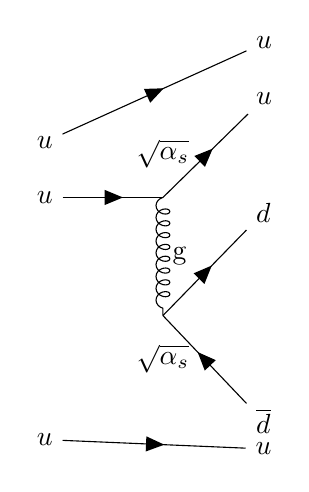
\begin{tikzpicture}
      \begin{feynman}
        \vertex (i1) {$u$};
       
        \vertex [right=of i1] (m1);
        \vertex [above=0.7 em of m1] {$\sqrt{\alpha_s}$};
        \vertex [above right=of m1] (f1) {$u$};
        \vertex [below=of m1] (m3);
        \vertex [below=0.7 em of m3] {$\sqrt{\alpha_s}$};
        \vertex [above right=of m3] (f2) {$d$};
        \vertex [below right=of m3] (f3) {$\overline{d}$};
         \vertex [below= 8.75 em of i1] (i2) {$u$};
        \vertex [right=of i2] (m2);
        \vertex [below=1 em of f3] (f4) {$u$};
        \vertex [above = 2em of f1](f5){$u$};
        \vertex [above = 2em of i1](i3){$u$};
        \diagram* {
          (i1) -- [fermion] (m1),
          (i2) -- [fermion] (f4),
          (m1) -- [fermion] (f1),
          (m1) -- [gluon, edge label = g] (m3),
          (m3) -- [fermion] (f2),
          (f3) -- [fermion] (m3),
          (i3) -- [fermion] (f5)
        };
      \end{feynman}
    \end{tikzpicture}
    
\begin{tabular}{|l|l|l|}
\hline
  & initial     & final      \\
  \hline
$J^P$     & $\frac{3}{2}^+$     &
$\frac{1}{2}^+$, $0^-$     \\
\hline
$P$ & $+1$ & $(-1)(-1)(-1)^L=+1$ \\
\hline
$J$& $0+\frac{3}{2}$ &should be 1\\
\hline
$m$ & 1231 MeV & 938 and 140 MeV respectively\\
\hline
\end{tabular}
\end{center}
We need $L=1$ to conserve parity, and this is consistent with conservation of $J$, i.e. $J=1$. This is an allowed process with $\mathcal{M}\propto\alpha_s$.
\end{eg}
We need to be careful if there are identical particles in the final state.
\begin{eg}[$\omega^0\rightarrow\pi^0\pi^0$]
Take $\omega^0$ and $\pi^0$ to be $u\overline{u}$.
\begin{center}
    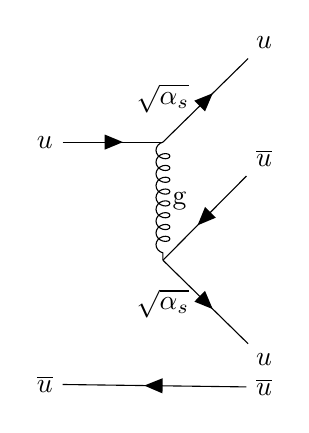
\begin{tikzpicture}
      \begin{feynman}
        \vertex (i1) {$u$};
       
        \vertex [right=of i1] (m1);
        \vertex [above=0.7 em of m1] {$\sqrt{\alpha_s}$};
        \vertex [above right=of m1] (f1) {$u$};
        \vertex [below=of m1] (m3);
        \vertex [below=0.7 em of m3] {$\sqrt{\alpha_s}$};
        \vertex [above right=of m3] (f2) {$\overline{u}$};
        \vertex [below right=of m3] (f3) {$u$};
         \vertex [below= 8.75 em of i1] (i2) {$\overline{u}$};
        \vertex [right=of i2] (m2);
        \vertex [below=1 em of f3] (f4) {$\overline{u}$};
        \diagram* {
          (i1) -- [fermion] (m1),
          (f4) -- [fermion] (i2),
          (m1) -- [fermion] (f1),
          (m1) -- [gluon, edge label = g] (m3),
          (f2) -- [fermion] (m3),
          (m3) -- [fermion] (f3)
        };
      \end{feynman}
    \end{tikzpicture}

\begin{tabular}{|l|l|l|}
\hline
  & initial     & final      \\
  \hline
$J^P$     & $1^-$     &
$0^-$, $0^-$     \\
\hline
$P$ & $-1$ & $(-1)(-1)(-1)^L=-1$ \\
\hline
$J$& $0+1$ &should be 1\\
\hline
$m$ & 782 MeV & 135 MeV each\\
\hline
\end{tabular}
\end{center}
We need $L=1$ to conserve parity, and this is consistent with conservation of $J$, i.e. $J=1$. But the final state consists of identical bosons and thus must be even under exchange, requiring even $L$, hence forbidden decay.
\end{eg}
\begin{eg}[$\omega^0\rightarrow\pi^+\pi^-\pi^0$]
Take $\omega^0$ and $\pi^0$ to be $u\overline{u}$, $\pi^+$ be $u\overline{d}$ and $\pi^-$ to be $d\overline{u}$.
\begin{center}
    \begin{tikzpicture}
      \begin{feynman}
        \vertex (i1) {$u$};
        \vertex [right=of i1] (m1);
        \vertex [above=0.7 em of m1] {$\sqrt{\alpha_s}$};
        \vertex [above right=of m1] (f1) {$u$};
        \vertex [below=of m1] (m2);
        \vertex [left=0.7 em of m2] {$\sqrt{\alpha_s}$};
        \vertex [above right=of m2] (f2) {$\overline{d}$};
        \vertex [right=of m2] (f3) {$d$};
        \vertex [below=1 em of m2] (m3);
        \vertex [left=0.7 em of m3] {$\sqrt{\alpha_s}$};
        \vertex [right=of m3] (f4) {$\overline{u}$};
        \vertex [below right=of m3] (f5) {$u$};
        \vertex [below=of m3] (m4);
        \vertex [below=0.7 em of m4] {$\sqrt{\alpha_s}$};
        \vertex [below right=of m4] (f6) {$\overline{u}$};
        \vertex [left=of m4] (i2) {$\overline{u}$};
        \diagram* {
          (i1) -- [fermion] (m1),
          (m1) -- [fermion] (f1),
          (f2) -- [fermion] (m2),
          (m2) -- [fermion] (f3),
          (m3) -- [fermion] (f5),
          (f4) -- [fermion] (m3),
          (f6) -- [fermion] (m4),
          (m4) -- [fermion] (i2)
          (m1) -- [gluon, edge label = g] (m2),
          (m3) -- [gluon, edge label = g] (m4)
        };
      \end{feynman}
    \end{tikzpicture}
    
\begin{tabular}{|l|l|l|}
\hline
  & initial     & final      \\
  \hline
$J^P$     & $1^-$     &
$0^-$, $0^-$, $0^-$     \\
\hline
$P$ & $-1$ & $(-1)(-1)(-1)(-1)^{L_{12}+L_3}=-1$ \\
\hline
$J$& $0+1$ &should be 1\\
\hline
$m$ & 782 MeV & 140, 140, 135 MeV\\
\hline
\end{tabular}
\end{center}
We need $L=1=L_{12}=L_3$ to conserve parity, and this is consistent with conservation of $J$, i.e. $J=1$. This is an allowed process with $\mathcal{M}\propto\alpha_s^2$.
\end{eg}
Hadrons can also decay via the electromagnetic interaction.
\begin{eg}[$\rho^0\rightarrow\pi^0\gamma$]
Take $\rho^0$ and $\pi^0$ to have composition $u\overline{u}$.
\begin{center}
    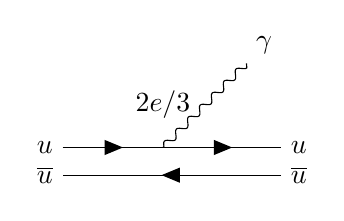
\begin{tikzpicture}
      \begin{feynman}
        \vertex (i1) {$u$};
        \vertex [below= 1 em of i1] (i2) {$\overline{u}$};
        \vertex [right=of i1] (m1);
        \vertex [above=0.7 em of m1] {$2e/3$};
        \vertex [above right=of m1] (f1) {$\gamma$};
        \vertex [right=of m1] (f2) {$u$};
        \vertex [right=of i2] (m2);
        \vertex [below =1em of f2] (f3) {$\overline{u}$};
        \diagram* {
          (i1) -- [fermion] (m1),
          (f3) -- [fermion] (i2),
          (m1) -- [photon] (f1),
          (m1) -- [fermion] (f2)
        };
      \end{feynman}
    \end{tikzpicture}

\begin{tabular}{|l|l|l|}
\hline
  & initial     & final      \\
  \hline
$J^P$     & $1^-$     &
$0^-$, $1^-$     \\
\hline
$P$ & $-1$ & $(-1)(-1)(-1)^L=-1$ \\
\hline
$J$& $0+1$ &should be 1\\
\hline
$m$ & 769 MeV & 135 and 0 MeV respectively\\
\hline
\end{tabular}
\end{center}
We need $L=1$ to conserve parity, and this is consistent with conservation of $J$, i.e. $J=1$. This is an allowed process with $\mathcal{M}\propto 2e/3$.
\end{eg}
\begin{eg}[$\Sigma^0\rightarrow\Lambda^0\gamma$]
Take $\Sigma^0$ and $\Lambda^0$ to have composition $uds$.
\begin{center}
    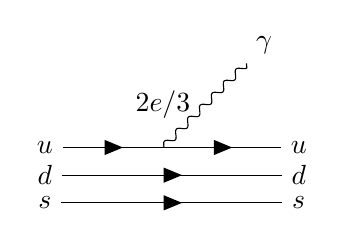
\begin{tikzpicture}
      \begin{feynman}
        \vertex (i1) {$u$};
        \vertex [below= 1 em of i1] (i2) {$d$};
        \vertex [below= 1 em of i2] (i3) {$s$};
        \vertex [right=of i1] (m1);
        \vertex [above=0.7 em of m1] {$2e/3$};
        \vertex [above right=of m1] (f1) {$\gamma$};
        \vertex [right=of m1] (f2) {$u$};
        \vertex [right=of i2] (m2);
        \vertex [below =1em of f2] (f3) {$d$};
         \vertex [below =1em of f3] (f4) {$s$};
        \diagram* {
          (i1) -- [fermion] (m1),
          (i2) -- [fermion] (f3),
          (m1) -- [photon] (f1),
          (m1) -- [fermion] (f2),
          (i3) -- [fermion] (f4)
        };
      \end{feynman}
    \end{tikzpicture}

\begin{tabular}{|l|l|l|}
\hline
  & initial     & final      \\
  \hline
$J^P$     & $\frac{1}{2}^+$     &
$\frac{1}{2}^+$, $1^-$     \\
\hline
$P$ & $+1$ & $(+1)(-1)(-1)^L=+1$ \\
\hline
$J$& $0+0.5$ &should be 0.5\\
\hline
$m$ & 1193 MeV & 1116 and 0 MeV respectively\\
\hline
\end{tabular}
\end{center}
We need $L=1$ to conserve parity, and this is consistent with conservation of $J$, i.e. $J=1/2$. This is an allowed process with $\mathcal{M}\propto 2e/3$.
\end{eg}
\begin{eg}[Spin of the pion]\leavevmode
\begin{itemize}
\item For charged pions, the spin was originally determined by measurement of the cross-section for the reversible reaction 
$$p+p\rightarrow\pi^++d$$
If the forward and backward reactions are compared at the same energy in the centre-of-momentum system, then $|\mathcal{M}_{if}|^2=|\mathcal{M}_{fi}|^2$. We have
$$\sigma_{\text{forward}}\propto(2s_\pi+1)(2s_d+1)p_\pi^2,\quad \sigma_{\pi^+d\rightarrow pp}\propto\frac{1}{2}(2s_p+1)^2p_p^2$$
where $p_\pi=p_d$ and the latter factor of $1/2$ arise since the two protons in the final state are identical. Since $s_d=1$, the ratio of the cross-section will give $s_\pi=0$.
\item For neutral pions, the existence of the decay
$$\pi^0\rightarrow 2\gamma$$
proves that the pion spin must be integral (since $s_\gamma=1$). We can show $s_\pi\neq 1$ and $s_\pi=0$ or $s_\pi\geq2$.\\[5pt]
For any massless particle of spin $s$, there are only two possible spin substates, $s_z=\pm s$, where $z$ is the direction of motion. Taking the common line of flight of the photons in the pion rest frame as the quantization axis, the $z$-component of total photon spin in the above decay can thus have the values $S_z=0$ or 2. Suppose $s_\pi=1$, then only $S_z=0$ is possible, and the two-photon amplitude must behave under rotation like the polynomial $P_1^m(\cos\theta)$ with $m=0$, where $\theta$ is the angle of the photon relative to the $z$-axis. Under exchange of two photons via $\theta\rightarrow\pi-\theta$, and since $P_1^0\propto\cos\theta$, it therefore changes sign. For $S_z=0$, the situation corresponds to two right (or left)-circularly polarized photons travelling in opposite directions. This is a contradiction since photons are bosons.
\end{itemize}
\end{eg}
\begin{eg}[Parity of charged pion]
Consider the reaction of slow negative pions captured in deuterium
$$\pi^-+d\rightarrow n+n$$
Since the spin is $s_d=1$ and $s_\pi=0$, the initial state has total angular momentum $J=1$. If the two neutrons have orbital angular momentum $\vec{L}$ and $\vec{S}$ is their total spin, then $\vec{J}=\vec{L}+\vec{S}$. The overall symmetry of the wavefunction of two neutrons under total interchange (space and spin) will be $(-1)^{S+1}(-1)^L$. For identical fermions, $\psi$ is antisymmetric, so $L+S$ must be even. The requirement $J=1$ and $L+S$ even only allow $L=S=1$. Since both neutron and the deuteron have intrinsic parity $+1$, then the only way to obtain negative parity in the initial state (total parity of two neutrons is $(+1)(+1)(-1)^L=-1$) is to assign $P_\pi=-1$.
\end{eg}
\newpage
\subsection{Heavy hadrons}
Very massive meson states were observed in the 1970s as sharp resonances in $e^+e^-$ annihilation at high energy. Their fine structure in several energy levels bore a remarkable resemblance to the levels of positronium (a non-relativistic bound state of $e^+$ and $e^-$), these heavy mesons must be evidence of bound states of massive fundamental fermion-antifermion pairs.
\begin{eg}[Charmonium]
The charmonium was first observed in 1974 at SLAC (Stanford) using the $e^+e^-$ collider SPEAR. Independently, it was also discovered in experiments at the Brookhaven alternating gradient synchrotron (AGS) in collisions of 28 GeV protons on a beryllium target, leading to a massive $e^+e^-$ pair. They were named J and $\psi$ respectively, and it is now known as $J/\psi$. $J/\psi$ is 3 times heavier than the proton but a thousand times longer lifetime. Only the quark model can account for this meson. The $J/\psi$ particle is the lowest energy bound unstable $c\overline{c}$ state.
\end{eg}
\begin{remarks}\leavevmode
\begin{enumerate}
\item Knowing the $c\overline{c}$ energy levels provides a probe of the QCD potential (determine empirically).
\item The width of $J/\psi$ peak depends on whether the decay to lightest mesons contianing $c$ quarks, $D^-(d\overline{c})$ and $D^+(c\overline{d})$ is kinematically possible or not. If $m(\psi)>2m(D)$, then reaction is allowed and hence large width. Unconnected lines int he Feynman diagram lead to suppression of the decay amplitude, hence narrow width (Zweig rule).
\item Expect to see charmed baryons and mesons - further extend quark symmetries to 3D (third direction is charm quantum number).
\item In Yukawa's original theory, the mediator of strong forces was the pion, but with the discovery of heavy mesons this simple picture could not stand. Protons and neutrons could now exchange $\rho$s, $\eta$s, $K$s and $\phi$s and all the rest of them. The quark model is needed and the strong force is due to the interaction between individual quarks.
\end{enumerate}
\end{remarks}
\begin{eg}
$\psi\rightarrow D^++D^-$ or $\psi\rightarrow D^0+\overline{D}^0$ is kinematically forbidden since a pair of D mesons weigh more. $\psi\rightarrow 3\pi$ is OZi suppressed. Hence, $\psi$ is very stable.
\end{eg}
\begin{eg}[Bottomium]
In 1977, similar narrow resonances in the mass region 9.5 to 10.5 GeV were discovered, attributed to bound states of heavy `bottom' quarks upsilon $\Upsilon$ (b$\overline{b}$).
\end{eg}
\begin{remarks}
Bottomonium spectrum well described by the same QCD potential as used for charmonium. This is evidence that the QCD potential does not depend on quark type. Can further extend quark symmetries to 4 dimensions.
\end{remarks}
\subsection{Flavour symmetries}
\begin{defi}[Isospin]
Isospin $\vec{I}$ was introduced with direct analogy to spin $\vec{S}$. The nucleon carries isospin $I=1/2$, with the proton and neutron respectively have $I_z=1/2$ and $I_z=-1/2$. Each of the multiplets in the Eightfold Way was assigned a particular isospin $I$ and to each member of the multiplet we assign a particular $I_z$ (plotted in the nonet, etc).
\end{defi}
\begin{remarks}
The strong force is invariant under rotations in the isospin space, hence isospin is conserved in all strong interactions.
\end{remarks}
\begin{eg}
In the pseudoscalar nonet of mesons, pions are assigned $I=1$, with $\pi^+$, $\pi^0$ and $\pi^-$ to be $|1,1\rangle$, $|1,0\rangle$ and $|1,-1\rangle$ respectively. In the decuplet of baryons, $\Delta$ are assigned $I=\frac{3}{2}$ with
$$\Delta^{++}=|1.5,1.5\rangle,\quad\Delta^+=|1.5,0.5\rangle,\quad\Delta^0=|1.5,-0.5\rangle,\quad\Delta^-=|1.5,-1.5\rangle$$
The number of particles in the multiplet is $2I+1$.
\end{eg}
\begin{remarks}[Gell-Mann-Nishijima formula]
The charge $Q$ is related to the isospin $I_3$ via $Q=I_3+0.5(A+S)$, where $A$ is the baryon number and $S$ is the strangeness.
\end{remarks}
\newpage
\section{Weak interaction}
\subsection{Weak force}
\begin{defi}[Weak interactions]
The weak interaction accounts for many decays in particle physics, characterized by long lifetimes and small interaction cross-sections.
\end{defi}
\begin{defi}[Charged current, neutral current]
Weak currents arise from the flow of conserved weak charge $g$. There are two types of weak interaction: charged current and neutral current mediated by massive $W^{\pm}$ and $Z$ bosons respectively. $W^\pm$ exchange results in a change of charge of the lepton or quark, while $Z^0$ exchange does not. Only the charged current weak interaction changes flavour, it is the only interaction that can violate parity conservation.
\end{defi}
\begin{remarks}
Neutral weak processes were only essential in the Glashow-Weinberg-Salam (GWS) model in 1958. Their existence was confirmed experimentally at CERN in 1973. They tend to be masked by much stronger electromagnetic effects. For instance, Z or photon can be exchanged between two electrons.
\end{remarks}
\begin{defi}[Boson self interaction]
The $W^\pm$ and $Z$ bosons carry the weak charge, while the $W^\pm$ further carry an electric charge. They do self-interact (either EM vertex for charged bosons or weak vertex for all).
\end{defi}
\begin{eg}
Comparing the weak decay $\Sigma^+\rightarrow p\pi_0$ with the electromagnetic decay $\Sigma^0\rightarrow\Lambda\gamma$, the weak coupling is smaller by a factor of order $\sqrt{10^{-19}/10^{-10}}\sim 10^{-5}$ than the electromagnetic coupling $\alpha$.
\end{eg}
\begin{remarks}
Usually, the weak interaction is completely swamped by the much greater strong and electromagnetic interactions, unless these are forbidden by some conservation rule. Observable weak interactions consequently involve either neutrinos or quarks with a flavour change that is forbidden for strong interactions.
\end{remarks}
\begin{eg}
A typical strong decay involves a lifetime around $10^{-23}$ s, electromagnetic decay $10^{-16}$ s, weak decay times range from around $10^{-13}$ s (for $\tau$) up to 15 min (for neutron). For a given type of decay, the decay generally proceeds more rapidly the larger the mass difference between the decay products and the original particles. However, $\pi^+\rightarrow\mu^+\nu_\mu$ is 10$^4$ times faster than $\pi^+\rightarrow e^+\nu_e$.
\end{eg}
\subsection{Fermi theory}
The weak interactions are weak principally because they are mediated by charged and neutral vector bosons $W^{\pm}$, $Z^0$, which are very massive (80 GeV and 91 GeV respectively) and hence give rise to interactions of very short range.
\begin{defi}[4-fermion contact interaction]
The old idea of weak interaction is a `4-fermion contact interaction' with
\begin{itemize}
    \item no propagator
    \item coupling strength given by the Fermi constant $G_F=1.166\times10^{-5}$ GeV$^{-2}$
\end{itemize}
Defining the weak charge $q$, the matrix element is $$\mathcal{M}=\frac{g^2}{q^2-M_{W,Z}^2}$$
For $q^2<<M_{W,Z}^2$, this is independent of $q^2$, i.e. the interaction is pointlike. Fermi postulated just such an interaction of strength $G$, between four fermions to describe nuclear $\beta$-decay back in 1934. At low $q^2$, we can write
$$G=\frac{g^2}{-M^2_{W,Z}}\approx 10^{-5}~\text{GeV}^{-2}$$
For $m_W=80.4$ GeV, the range is $1/m_W\sim$ 0.002 fm. It is thus a low energy effective theory of the weak interaction.
\end{defi}
\begin{eg}
Historically, the prototype weak interaction was nuclear $\beta$-decay, e.g. the decay of a free or bound neutron. In terms of quark constituents,
$$d\rightarrow u+e^-+\overline{\nu}_e$$
The interaction is effectively pointlike and described by the apparent four-fermion coupling, postulated by Fermi in 1934.
\end{eg}
\begin{remarks}\leavevmode
\begin{enumerate}
\item Fermi theory is wrong. Consider
$$\nu_e+n\rightarrow p+e^-$$
The matrix element of the 4-point interaction is $G_F^2$ since there are a total of 4 possible spin states for the spin $\frac{1}{2}$ e and $\nu$. The cross-section is
$$d\sigma=2\pi|\mathcal{M}_{fi}|^2\frac{dN}{dE}=2\pi 4G_F^2\frac{E_e^2}{(2\pi)^3}d\Omega\implies\sigma=\int\frac{G_F^2E_e^2}{\pi^2}d\Omega=\frac{G_F^2s}{\pi}$$
where $E_e$ is the energy of the electron in the centre-of-mass system and $\sqrt{s}=2E_e$ is the energy in the centre-of-mass system. In the laboratory frame, $s=2E_\nu m_n$ (fixed target collision), so $\sigma\sim (E_\nu/\text{MeV})\times10^{-43}$ cm$^{-2}$, i.e. neutrinos only interact weakly. However, as $E_\nu\rightarrow\infty$, $\sigma\rightarrow\infty$. At sufficiently large energy, the Fermi theory therefore predicts a cross-section exceeding the wave-theory limit, which is determined by the condition that the scattered intensity cannot exceed the incident intensity in any partial wave, i.e. unitarity limit - violating the maximum value allowed by the conservation of probability at $\sqrt{s}\sim 1$ TeV.
\item Compare Fermi theory with a massive propagator. For $q<<m_W^2$, the precise relationship when comparing matrix elements is 
$$\frac{g_W^2}{8m_W^2}\rightarrow\frac{G_F}{\sqrt{2}}$$
$G_F$ is small because $m_W$ is large. Compute the intrinsic strength:
$$m_W=80.4\text{GeV},~G_F=1.166\times10^{-5}\text{GeV}^{-2}\implies g_W=0.65\implies\alpha_W=\frac{g_W^2}{4\pi}\sim\frac{1}{30}>\alpha$$
The intrinsic strength of the weak interaction is actually greater than that of the electromagnetic interaction.
\end{enumerate}
\end{remarks}
\begin{eg}[Neutrino scattering with a massive W boson]
Compare Fermi theory and Standard model prediction for the differential cross-section:
$$\frac{d\sigma}{d\Omega}=2\pi G_F^2\frac{E_e^2}{(2\pi)^3},\quad\frac{d\sigma}{d\Omega}=2\pi G_F^2\frac{E_e^2}{(2\pi)^3}\bigg(\frac{m_W^2}{m_W^2-q^2}\bigg)^2$$
with $|\vec{q}|^2=4E_e^2\sin^2\theta/2$ where $\theta$ is the scattering angle. Integrate to give
$$\sigma=\int\frac{G_F^2s}{4\pi^2}\bigg(\frac{m_W^2}{m_W^2+|q|^2}\bigg)^2d\Omega=\frac{G_F^2m_W^4}{\pi}\int_0^s\frac{du}{(m_W^2+u)^2}=\frac{G_F^2m_W^4}{\pi}\bigg(\frac{1}{m_W^2}-\frac{1}{m_W^2+s}\bigg)=\frac{G_F^2m_W^2s}{\pi(m_W^2+s)}$$
For $s<<m_W^2$, we recover the Fermi theory result $\sigma=G_F^2s/\pi$. But, $\sigma=\frac{G_F^2m_W^2}{\pi}$ for $s>>m_W^2$. Cross-section is now well-behaved at high energies.
\end{eg}
\newpage
\subsection{C-symmetry and parity violation}
\begin{defi}[Helicity]
Helicity $H$ measures the sign of the component of spin of the particle $j_z=\pm\hbar/2$ in the direction of motion (z-direction). 
\begin{equation}
    H=\frac{\vec{S}\cdot\vec{p}}{|\vec{p}|}=-1\label{helicity}
\end{equation}
The z-component of spin and $\vec{p}$ together define a screw sense, $H=+1$ and $-1$ correspond to a right-handed RH and left-handed LH screw.
\end{defi}
\begin{eg}[Wu experiment]
Radioactive Cobalt 60 nuclei were carefully aligned by $\vec{B}$ field, so that their spins pointed in say, the $z$ direction. It undergoes beta decay, and Wu recorded the direction of the emitted electrons, i.e.  $^{60}$Co$\rightarrow$ $^{60}$Ni+e$^-+\overline{\nu}_e$. $e^-$ is always observed in the direction opposite to spin (left-handed). By $\vec{p}$ conservation, $\overline{\nu}$ must be emitted in the opposite direction (hence right-handed). Right-handed electrons are not observed here. So if helicity is not conserved, $\vec{J}$ is not conserved. To conserve $\vec{J}$, $\vec{L}$ must change, i.e. parity changes in the weak interaction.
\end{eg}
\begin{remarks}\leavevmode
\begin{enumerate}
\item The total angular momentum $\vec{J}=\vec{L}+\vec{S}=\vec{r}\times\vec{p}+\vec{S}$ is always conserved. The value of $\vec{S}$ along $\vec{p}$ is always constant.
\item Helicity is a well-defined, Lorentz invariant quantity for a massless particle since such a particle travels at velocity $c$. In making a Lorentz transformation to another reference frame of relative velocity $v<c$, it is therefore impossible to reverse the helicity. 
\item For interactions involving vector or axial vector fields (mediated by vector or axial vector bosons), helicity is conserved in the relativistic limit, thus applies to strong, weak and electromagnetic interactions. A LH lepton, undergoing scattering in such an interaction, will emerge as a LH particle, irrespective of the angle of scatter, provided it is extremely relativistic.
\item A scalar interaction does not preserve the helicity and does mix LH and RH states. Example of scalar field particles is the Higgs boson.
\end{enumerate}
\end{remarks}
\begin{eg}
Of all the fundamental fermions, neutrinos are unique in that they are completely longitudinally polarized. Only the projection $j_z=-\hbar/2$ is observed, corresponding to the pure helicity state $H=-1$. Neutrino is said to be LH, while anti-neutrino is RH. Such pure helicity states are only possible for strictly massless particles, by Lorentz invariance. A massless neutrino thus cannot possess a magnetic dipole moment, since if it did the spin direction could be flipped by an applied magnetic field.
\end{eg}
\begin{remarks}
The weak interaction distinguishes between left- and right-handed states by coupling preferentially to left-handed particles and right-handed anti-particles. This experimental observation has to be built into the Standard Model. The probability for weak coupling to the $\pm$ helicity state is
$$\frac{1}{2}(1\mp\frac{v}{c}),\quad\frac{1}{2}(1\pm\frac{v}{c}\bigg)$$
for a lepton and an anti-lepton respectively. Coupling to right-handed particles and left-handed antiparticles vanishes.
\end{remarks}
\begin{defi}[Charge conjugation]
The operation of charge conjugation reverses the sign of the charge and magnetic moment of a particle, leaving all other coordinates unchanged.
\end{defi}
\begin{eg}\leavevmode
\begin{enumerate}
    \item Strong and electromagnetic interactions are found experimentally to be invariant under the charge conjugation operation.
    \item Only neutral bosons that are their own antiparticles can be eigenstates of the charge conjugation operator.
    \item C invariance is broken in weak interactions. Under the C operation, a LH neutrino $\nu$ will transform into a LH antineutrino $\overline{\nu}$ which is not found in nature. 
\end{enumerate}
\end{eg}
\begin{remarks}
It is under the combined operation CP, a LH neutrino $\nu_L$ is transformed into a RH anti-neutrino $\overline{\nu}_R$. Hence, are eigenstates of the product CP. Remarkably, CP violation in weak interactions still does occur, at the 10$^{-4}$ level - neutral Kaons experiment.
\end{remarks}
\begin{eg}
Consider the decay of $\eta$ (u$\overline{u}$) which can either give $\pi^0\pi^0\pi^0$ or $\pi^+\pi^-$. For the former:
\begin{center}
        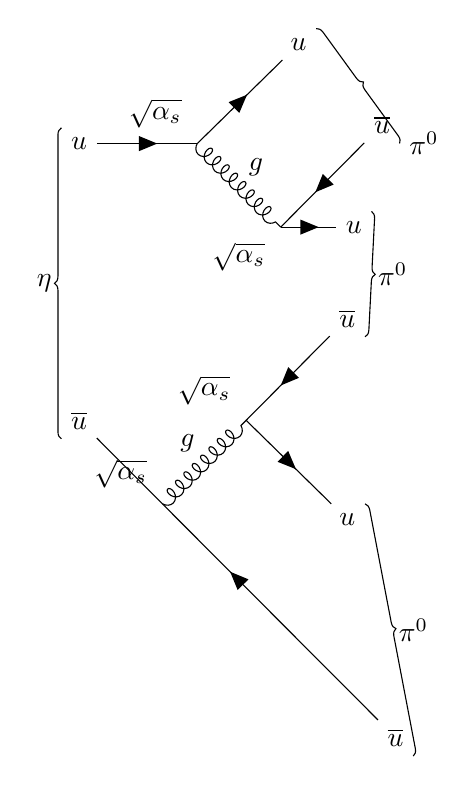
\begin{tikzpicture}
      \begin{feynman}
        \vertex (i1) {$u$};
        \vertex [right=of i1] (m1);
        \vertex [above left=0.3 em of m1] {$\sqrt{\alpha_s}$};
        \vertex [above right=of m1] (f1) {$u$};
        \vertex [below right=of m1] (m3);
        \vertex [below left=0.3 em of m3] {$\sqrt{\alpha_s}$};
        \vertex [above right=of m3] (f2) {$\overline{u}$};
        \vertex [right = 2 em of m3] (f3) {$u$};
         \vertex [below= 10 em of i1] (i2) {$\overline{u}$};
        \vertex [below right= of i2] (m4);
        \vertex [above left=0.3 em of m4] {$\sqrt{\alpha_s}$};
        \vertex [below right= 11 em of m4] (f6) {$\overline{u}$};
        \vertex [above right= of m4] (m5);
        \vertex [above left=0.3 em of m5] {$\sqrt{\alpha_s}$};
        \vertex [above right = of m5] (f4) {$\overline{u}$};
        \vertex [below right = of m5] (f5) {$u$};
        \diagram* {
          (i1) -- [fermion] (m1),
          (f6) -- [fermion] (i2),
          (m1) -- [fermion] (f1),
          (m1) -- [gluon, edge label = $g$] (m3),
          (f2) -- [fermion] (m3),
          (m3) -- [fermion] (f3),
          (m4) -- [gluon, edge label = $g$] (m5),
          (f4) -- [fermion] (m5),
          (m5) -- [fermion] (f5)
        };
        \draw [decoration={brace}, decorate]  (i2.south west) --  (i1.north west)
          node [pos=0.5, left] {$\eta$};
          
        \draw [decoration={brace}, decorate] (f3.north east) --  (f4.south east)
          node [pos=0.5, right] {$\pi^0$};
        \draw [decoration={brace}, decorate] (f5.north east) --  (f6.south east)
          node [pos=0.5, right] {$\pi^0$};
           \draw [decoration={brace}, decorate] (f1.north east) -- (f2.south east)
          node [pos=1, right] {$\pi^0$};
      \end{feynman}
    \end{tikzpicture}
    \end{center}
    \begin{center}
        \begin{tabular}{|c|c|c|}
        \hline
             & Initial & Final \\
             \hline
            $J^P$ & $0^-$ & $0^- 0^-$\\
            \hline
            P & -1 & $(-1)(-1)(-1)^{L_{12}+L_3}$\\
            \hline
            J & 0+0 & $|L-0|\dots|L+0|$\\
            \hline
        \end{tabular}
    \end{center}
    $L$ needs to be even for partiy conservation. $L$ needs to be zero to conserve $J$. This is allowed, with branching ratio of 32\%.\\[5pt]
    For the latter: 
      \begin{center}
        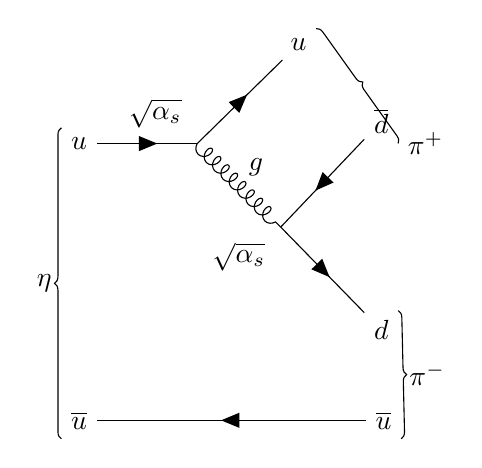
\begin{tikzpicture}
      \begin{feynman}
        \vertex (i1) {$u$};
        \vertex [right=of i1] (m1);
        \vertex [above left=0.3 em of m1] {$\sqrt{\alpha_s}$};
        \vertex [above right=of m1] (f1) {$u$};
        \vertex [below right=of m1] (m3);
        \vertex [below left=0.3 em of m3] {$\sqrt{\alpha_s}$};
        \vertex [above right=of m3] (f2) {$\overline{d}$};
        \vertex [below right=of m3] (f3) {$d$};
         \vertex [below= 10 em of i1] (si1) {$\overline{u}$};
        \vertex [right= 11 em of si1] (sf1) {$\overline{u}$};
        \diagram* {
          (i1) -- [fermion] (m1),
          (sf1) -- [fermion] (si1),
          (m1) -- [fermion] (f1),
          (m1) -- [gluon, edge label = $g$] (m3),
          (f2) -- [fermion] (m3),
          (m3) -- [fermion] (f3)
        };
        \draw [decoration={brace}, decorate]  (si1.south west) --  (i1.north west)
          node [pos=0.5, left] {$\eta$};
        \draw [decoration={brace}, decorate] (f3.north east) --  (sf1.south east)
          node [pos=0.5, right] {$\pi^-$};
           \draw [decoration={brace}, decorate] (f1.north east) -- (f2.south east)
          node [pos=1, right] {$\pi^+$};
      \end{feynman}
    \end{tikzpicture}
    \end{center}
    \begin{center}
        \begin{tabular}{|c|c|c|}
        \hline
             & Initial & Final \\
             \hline
            $J^P$ & $0^-$ & $0^- 0^-$\\
            \hline
            P & -1 & $(-1)(-1)(-1)^L$\\
            \hline
            J & 0+0 & $|L-0|\dots|L+0|$\\
            \hline
        \end{tabular}
    \end{center}
    $L$ needs to be odd for partiy conservation. But $L$ needs to be zero to conserve $J$. Hence, parity violated in this strong interaction and this reaction is not observed (branching ratio of less than 0.1\%.
\end{eg}
\newpage
\subsection{Lepton universality}
\begin{defi}[Weak interactions of leptons]
All weak charged current lepton interactions can be described by the W boson propagator and the weak vertex. W bosons only `couple' to the left-handed lepton and neutrino within the same generation
$$\begin{pmatrix}e^-\\\nu_e\\\end{pmatrix},\quad\begin{pmatrix}\mu^-\\\nu_\mu\\\end{pmatrix},\quad\begin{pmatrix}\tau^-\\\nu_\tau\\\end{pmatrix}$$
with coupling constant $g_W=\sqrt{4\pi\alpha_W}$.
\end{defi}
\begin{eg}[$\mu$ decay]
Electromagnetic decay $\mu^-\rightarrow e^-\gamma$ is not observed since the EM interaction does not change flavour. Only the weak charged current interaction changes lepton type, but only within a generation. Lepton number is still conserved for each lepton generation. As $m_\mu<<m_W$, we can safely use Fermi theory to calculate decay width: $\propto m_\mu^5$ (Sargent rule). More complicated phase space integration (include kinetic energy of recoiling nucleus, helicity and spin) gives
$$\Gamma_\mu=\frac{1}{\tau_\mu}=\frac{G_F^2m_\mu^5}{192\pi^3}$$
giving $m_\mu=(105.6583715\pm0.0000035)$ MeV and $\tau_\mu=(2.1969811\pm0.0000022)\times10^{-6}$ s, hence $G_F=(1.16632\pm0.00002)\times10^{-5}$ GeV$^{-2}$.
\end{eg}
\begin{eg}[$\tau$ decay]
Since $m_\tau\rightarrow m_\mu, m_\pi,m_p$, there are three decay modes with branching fractions:
\begin{center}
    \begin{tabular}{cc}
         $\tau^-\rightarrow e^-\overline{\nu}_e\nu_\tau$& 17.83$\pm$0.04\%  \\
        $\tau^-\rightarrow \mu^-\overline{\nu}_\mu\nu_\tau$& 17.41$\pm$0.04\%  \\
        $\tau^-\rightarrow \text{hadrons}$& 64.76$\pm$0.06\%  \\
    \end{tabular}
\end{center}
\end{eg}
\begin{prop}
Weak charged current coupling is the same for all leptons.
\end{prop}
\begin{eg}
Consider the decays $\mu\rightarrow e$ and $\tau\rightarrow e$, we have
$$\frac{1}{\tau_\mu}=\Gamma_{\mu\rightarrow e}=\frac{G_F^2}{192\pi^3}m_\mu^5,\quad\frac{1}{\tau_\tau}=\frac{\Gamma_{\tau\rightarrow e}}{B(\tau\rightarrow e)}=\frac{1}{0.178}\frac{G_F^2}{192\pi^3}m_\tau^5$$
If the weak interaction strength is universal, we expect $\frac{\tau_\tau}{\tau_\mu}=0.178\frac{m_\mu^5}{m_\tau^5}$. With $m_\mu=(105.6583715\pm0.0000035)$ MeV, $m_\tau=(1.77686\pm0.00012)$ GeV and $\tau_\mu=(2.1969811\pm0.0000022)\times10^{-6}$ s, we predict $\tau_\tau=(2.903\pm0.005)\times10^{-13}$ s, which agrees with the measured value.
\end{eg}
\begin{eg}
Consider $\tau^-\rightarrow\mu^-$ and $\tau^-\rightarrow e^-$, if the couplings are the same, we expect
$$\frac{B(\tau^-\rightarrow\mu^-\overline{\nu}_\mu\nu_\tau)}{B(\tau^-\rightarrow e^-\overline{\nu}_e\nu_\tau}=0.9726$$
which is close to the measured value of 0.974$\pm$ 0.005. The small disparity is due to the slight reduction in phase space due to the non-negligible muon mass.
\end{eg}
\begin{eg}
Compare $G_F$ measured from $\mu^-$ decay with that from nuclear $\beta$ decay:
$$G_F^\mu=(1.16632\pm0.00002)\times10^{-5}~\text{GeV}^{-2},\quad G_F^\beta=(1.136\pm0.003)\times10^{-5}~\text{GeV}^{-2}$$
Their ratio is 0.974$\pm0.003$, i.e. almost the same for leptons as for quarks. But, the difference is significant and has to be explained.
\end{eg}
\newpage
\subsection{Quark mixing}
\begin{eg}
Typically, weak charged current couplings take place within one generation of quarks. $\pi^+$ (u$\overline{d}$) may decay to $\mu^+\nu_\mu$, but not $K^+$ (u$\overline{s}$). The latter is still observed but much smaller.
\end{eg}
\begin{defi}[Weak interactions of quarks]
It was originally proposed that weak charged current couplings take place within one generation of quarks:
$$\begin{pmatrix}u\\d\\\end{pmatrix},\quad\begin{pmatrix}c\\s\\\end{pmatrix},\quad\begin{pmatrix}t\\b\\\end{pmatrix}$$
To account for experimental observations, we have to alter the lepton-quark symmetry. Consider quark mixing between first and second generation only:
$$\begin{pmatrix}u\\d'\\\end{pmatrix},~\begin{pmatrix}c\\s'\\\end{pmatrix},~d'=d\cos\theta_C+s\sin\theta_C,~s'=-d\sin\theta_C+s\cos\theta_C$$
The weak eigenstates $(d',s')$ are superpositions of the mass eigenstates $(d,s)$, with $\theta_C\sim 13\degree$ being the Cabibbo angle.
\end{defi}
\begin{eg}
Quark mixing explains the lower rate of $K^+\rightarrow\mu^+\nu_\mu$, compared to $\pi^+\rightarrow\mu^+\nu_\mu$, and the ratio is
$$\frac{G_F^\beta}{G_F^\mu}=\cos\theta_C$$
consistent with experimental value of 0.974.
\end{eg}
\begin{defi}[Cabibbo-Kobayashi-Maskawa matrix]
We can extend quark mixing to three generations.
$$\begin{pmatrix}d'\\s'\\b'\\\end{pmatrix}=V_{\text{CKM}}\begin{pmatrix}d\\s\\b\\\end{pmatrix},\quad V_{\text{CKM}}\sim\begin{pmatrix}\cos\theta_C&\sin\theta_C&\sin^3\theta_C\\-\sin\theta_C&\cos\theta_C&\sin^2\theta_C\\\sin^3\theta_C&-\sin^2\theta_C&1\\\end{pmatrix}$$
\end{defi}
\begin{remarks}
Weak interactions between quarks of the same family are 'Cabibbo allowed', i.e. $V_{\text{ud}},V_{\text{cs}},V_{\text{tb}}$. Between quarks differing by one family, it is `Cabibbo suppressed', i.e. $V_{\text{us}},V_{\text{cd}},V_{\text{cb}},V_{\text{ts}}$. Between quarks differing by two families are `doubly Cabibbo suppressed', i.e. $V_{\text{ub}},V_{\text{dt}}$.
\end{remarks}
\begin{eg}\leavevmode
\begin{enumerate}
\item $K^+\rightarrow\mu^+\nu_\mu$ involves coupling between $u\overline{s}$, hence Cabibbo suppressed. 
\item Consider the decays $D^0\rightarrow K^\mp\pi^\pm$. We expect the ratio to be
$$\frac{\Gamma(D^0\rightarrow K^+\pi^-)}{\Gamma(D^0\rightarrow K^-\pi^+)}\sim\frac{(g_W^2V_{\text{cd}}V_{\text{us}})^2}{(g_W^2V_{\text{cs}}V_{\text{ud}})^2}=\frac{\sin^4\theta_C}{\cos^4\theta_C}\sim 0.0028$$
$D^0\rightarrow K^+\pi^-$ is doubly Cabibbo suppressed.

\end{enumerate}
\end{eg}
\newpage
\section{Electroweak unification}
\subsection{GWS model}
\begin{eg}
Consider $e^-e^+\rightarrow W^+W^-$. $W^\pm$ bosons are charged, so they may couple to the $\gamma$. Two possible diagrams: t-channel exchanging $\nu_e$ or s-channel exchanging $\gamma$. But the cross-section diverges at high energy. To resolve this, introduce another diagram, exchanging the Z boson. This only works if $\gamma$, $W^\pm$ and $Z$ couplings are related. 
\end{eg}
\begin{remarks}
Electroweak gauge theory is postulated to be invariant under the gauge transformation (SU(2))
$$\psi\rightarrow\psi'=e^{ig\vec{\sigma}\cdot\vec{\Lambda}(\vec{r},t)}\psi$$
which operators on the state of `weak isospin'. This gives three massless gauge bosons ($W_1,W_2,W_3$) whose couplings are well-specified and have self-couplings. But this does not work. It predicts W and Z have the same couplings, which are not seen experimentally.\\[5pt]
The solution is to unify QED and weak force, i.e. invariant under SU(2)$\times$ U(1) transformation, former operating on the state of `weak isospin $I$' and latter operating on the `weak hypercharge' $Y=2(Q-I_3)$.\\[5pt]
This gives four massless gauge bosons $W^+$, $W^-$, $W_3$ and $B$. The $W$ bosons are the components of an $I=1$ triplet of the group SU(2), while the fourth $B$ is an isoscalar $I=0$ belonging to the U(1) group of weak hypercharge.\\[5pt]
A process called `spontaneous symmetry breaking' is invoked to endow the bosons with mass. The neutral bosons $W_3$ and $B$ mix to give $Z$ and $\gamma$. $\gamma$ is predicted from QED, so the predictions of the couplings of the $Z$ is in terms of those of the $W$ and $\gamma$.
\end{remarks}
\begin{defi}[Electroweak theory]
The electroweak theory of Glashow, Weinberg and Salam proposed over the period 1961-8 that the coupling $g$ of the $W^{\pm}$ and $Z^0$ to leptons and quarks should be the same as that of the photon, i.e. unifying weak and electromagnetic interactions with the same coupling. We expect
$$M_{W,Z}\sim\frac{e}{\sqrt{G}}\sim 90 GeV$$
Start with 4 massless bosons that mix to give physical bosons. The physical fields are related via:
$$Z=W_3\cos\theta_W-B\sin\theta_W,\quad A=W_3\sin\theta_W+B\cos\theta_W$$
where $A$ is the vector field of the photon. $W^\pm$ and $Z$ acquire mass via the Higgs mechanism (later). 
\end{defi}
\begin{remarks}\leavevmode
\begin{enumerate}
\item The GWS model makes exact predictions of the $W^\pm$ and $Z$ masses and of their couplings with only 3 free parameters. The couplings are given by
$$\alpha_EM=\frac{e^2}{4\pi}\implies g\sim e,\quad g_W=\frac{e}{\sin\theta_W},\quad g_Z=\frac{e}{\sin\theta_W\cos\theta_W}$$
The masses are given by:
$$\frac{G_F}{\sqrt{2}}=\frac{g_W^2}{8m_W^2}=\frac{e^2}{8m_W^2\sin^2\theta_W},\quad m_{W^\pm}=\bigg(\frac{\sqrt{2}e^2}{8G_F\sin^2\theta_W}\bigg)^{1/2},\quad m_Z=\frac{m_W}{\cos\theta_W}$$
\item $W_3$ couples to $I_3$ with strength $g_W$ and $B$ couples to $Y=2(Q-I_3)$ with $g'$. For right-handed fermions, $I_3=0$.
\end{enumerate}
\end{remarks}
\begin{eg}[Evidence for GWS model]\leavevmode
\begin{enumerate}
    \item $\overline{\nu}_\mu e^-\rightarrow\overline{\nu}_\mu e^-$ was observed. Only possible Feynman diagram involves exchange of $Z$ boson (indirect evidence).
    \item First direct observation in $p\overline{p}$ collisions at $\sqrt{s}=540$ GeV via decays into leptons $p\overline{p}\rightarrow W^{\pm}+X$ and $p\overline{p}\rightarrow Z+X$.
    \item LEP $e^+e^-$ collider provided many precision measurements of the Standard Model. 
    \item Wide variety of different processes consistent with GWS model predictions and measure same value of $\theta_W\sim 29\degree$.
\end{enumerate}
\end{eg}
\newpage
\begin{eg}
Assign the lepton states to a LH doublet and a RH singlet:
$$\psi_L=\begin{pmatrix}\nu_e\\e^-\\\end{pmatrix}_L,\quad I=\frac{1}{2},~I_3=\pm\frac{1}{2},~Q=0,-1\implies Y=-\frac{1}{2}$$
$$\psi_R=\begin{pmatrix}e^-\\\end{pmatrix}_R,\quad I=0,~Q=-1\implies Y=-1$$
The left-handed and right-handed couplings of the fermions to the $Z^0$ (neutral current) have the coefficients
$$g_L=I_3-Q\sin^2\theta_W,\quad g_R=-Q\sin^2\theta_W$$
where $Q$ is the electric charge in units of $|e|$ and $I_3=\pm\frac{1}{2}$ is the third component of the weak isospin. 
\end{eg}
\subsection{Allowed vertices}
\begin{defi}[Weak NC vertex]
All weak neutral current interactions can be described by the Z boson propagator and the weak vertices. Z never changes type of particle, quark or lepton flavour. Z couplings are a mixture of EM and weak couplings, and therefore dpeend on $\sin^2\theta_W$.
\end{defi}
\begin{eg}[$\pi^-p\rightarrow K^0\Lambda$]
Strong, EM or weak. Strong dominant since weak suppressed by change of flavour $\overline{u}u\rightarrow s\overline{s}$
\end{eg}
\begin{eg}[$\nu_\tau e^-\rightarrow\nu_\tau e^-$]
Only weak, via neutral current (since different generation of lepton). No s-channel since it is not the same generation, can only occur via t-channel.
\end{eg}
\begin{eg}[$\nu_\tau e^-\rightarrow\nu_\tau e^-$]
Same generation of leptons. Only weak, either via charged or neutral current. No t-channel for W since need to conserve charge. No s-channel for Z since need to conserve charge.
\end{eg}
\subsection{Experimental tests}
\begin{eg}[LEP]
Large electron positron (LEP) collider at CERN provided a Z and $W^{\pm}$ boson factory, and facilitate precise measurements of the properties of Z and $W^{\pm}$ bosons. $\sqrt{s}=90$ to 209 GeV. OPAL was one of the 4 experiments at the LEP.
\end{eg}
\begin{eg}
Consider the process $e^+e^-\rightarrow q\overline{q}$. At small $\sqrt{s}$ ($<50$ GeV), we only considered an intermediate photon. At higher energies, the Z exchange diagram contributes.
$$\sigma(e^+e^-\rightarrow\gamma\rightarrow q\overline{q})=\frac{4\pi\alpha^2}{3s}\sum 3Q_q^2$$
The $Z$ is a decaying intermediate massive state with lifetime $\sim 10^{-25}$ s. Around $\sqrt{s}\sim m_Z$, the Z diagram dominates. The Breit-Wigner cross-section for $e^+e^-\rightarrow Z\rightarrow f\overline{f}$, i.e. any fermion-antifermion pair. 
$$\sigma(e^+e^-\rightarrow Z\rightarrow f\overline{f})=\frac{3\pi}{4E_e^2}\frac{\Gamma_{\text{ee}}\Gamma_{f\overline{f}}}{(\sqrt{s}-m_Z)^2+(\Gamma_Z^2/4)}$$
We have $\sqrt{s}=E_{\text{CM}}=E_{e^+}+E_{e^-}$, $g=\frac{2J_Z+1}{(2J_{e^-}+1)(2J_{e^+}+1)}=\frac{3}{4}$, where $J_Z=1,J_{e^\pm}=1/2$. This gives
$$\sigma(e^+e^-\rightarrow Z\rightarrow f\overline{f})=\frac{3\pi}{s}\frac{\Gamma_{\text{ee}}\Gamma_{f\overline{f}}}{(\sqrt{s}-m_Z)^2+(\Gamma_Z^2/4)}$$
where $\Gamma_Z$ is the total decay width (sum over all decay modes - all leptons, quarks and neutrinos). At the peak of the resonance $\sqrt{s}=m_Z$, the cross-section for all fermion/anti-fermion pairs in the final state
$$\sigma=\frac{12\pi\Gamma_{\text{ee}}}{m_Z^2\Gamma_Z}$$
where $\Gamma_{f\overline{f}}=\Gamma_Z$. Compare to the QED cross-section at $\sqrt{s}=m_Z$, $\sigma_{\text{QED}}=4\pi\alpha^2/3s$, we have the ratio to be $\frac{9\Gamma_{\text{ee}}}{\alpha^2\Gamma_Z}\sim5700$. Run LEP at various centre-of-mass energies $\sqrt{s}$ close to the peak of the Z resonance and measure $\sigma(e^+e^-\rightarrow q\overline{q})$ to determine the parameters of the resonance - a central mass $m_Z=(91.1875\pm0.0021)$ GeV, peak cross-section $\sigma_{\text{max}}(q\overline{q})=(41.450\pm0.037)$ nb and a total width $\Gamma=(2.4952\pm0.0023)$ GeV.
\end{eg}
\begin{remarks}\leavevmode
\begin{enumerate}
\item We need to correct measurements for QED effects due to radiation from the $e^+e^-$ beams. This radiation has the effect of reducing the centre-of-mass energy of the $e^+e^-$ collision which smears out the resonance. 
\item Further, we need a detailed understanding of the accelerator and astrophysics. Tidal distortions of the Earth by the Moon distorts the rocks surrounding LEP, stretching the radius by 0.15 nm, in turn changing $\sqrt{s}$. We also need the train timetable. Leakage currents from the TGV rail via Lake Geneva follow the path of least resistance.
\end{enumerate}
\end{remarks}

\begin{eg}[Number of neutrino generations]
The $Z$, once formed, can decay to hadrons via $q\overline{q}$ pairs, into charged leptons $e^+e^-$, $\mu^+\mu^-$, $\tau^+\tau^-$ or into neutral lepton pairs $\nu_e\overline{\nu}_e$, $\nu_\mu\overline{\nu}_\mu$ and $\nu_\tau\overline{\nu}_\tau$, i.e. couple to all fermions. The total width is the sum of the individual partial widths for each decay mode. 
$$\Gamma_Z=\Gamma_{ee}+\Gamma_{\mu\mu}+\Gamma_{\tau\tau}+\Gamma_{q\overline{q}}+\sum_i\Gamma_{\nu_i\overline{\nu}_i}$$
The neutrinos would not be observed directly, but could infer their presence from the effect on the Z resonance curve. At the peak of the Z resonance, $\sqrt{s}=m_Z$, 
$$\sigma_{\text{max}}(f\overline{f})=\frac{12\pi\Gamma_{ee}\Gamma_{f\overline{f}}}{m_Z^2\Gamma_Z^2}$$
Measure the $e^+e^-\rightarrow Z\rightarrow f\overline{f}$ cross-sections for all visible decay modes, hence obtaining $\Gamma_{f\overline{f}}$. $\Gamma_{\text{ee}}$ obtained from $\sigma_{\text{max}}(ee)=\frac{12\pi\Gamma_{ee}^2}{m_Z^2\Gamma_Z^2}$.
The observed width gives the number of flavours to be $N_\nu=\frac{\Gamma_{\nu\nu}^{\text{measured}}}{\Gamma_{\nu\nu}^{\text{SM}}}=2.99\pm 0.01$, i.e. only three types of neutrinos lighter than $m_Z/2$.
\end{eg}
\begin{remarks}
Measurements of $\Gamma_{\text{ee}},\Gamma_{\mu\mu},\Gamma_{\tau\tau}$ are consistent with universality of the lepton couplings to the Z boson. $\Gamma_{qq}$ is consistent with the expected value which assumes 3 colours - further evidence for colour.
\end{remarks}
In $e^+e^-$ collisions, $W$ bosons are produced in piars with three possible diagrams: 't-channel' exchanging $\nu_e$, `s-channels' exchanging $\gamma$ or Z. The LEP has to operate above the threshold $\sqrt{s}>2m_W$.
\begin{eg}
In the standard model, $W\ell\nu$ and $Wq\overline{q}$ couplings are equal. Assuming three colours, we expect
$$B(W^\pm\rightarrow q\overline{q})=\frac{6}{9},\quad B(W^\pm\rightarrow\ell\nu)=\frac{3}{9}$$
Include further QCD corrections to obtain $B(W^\pm\rightarrow q\overline{q})=0.675$.
\end{eg}
\begin{remarks}
Unlike $e^+e^-\rightarrow Z$, W boson production at LEP was not a resonant process. $m_W$ was measured by measuring the invariant mass in each event. Measurement gives $m_W=(80.423\pm 0.038)$ GeV and $\Gamma_W=(2.12\pm0.11)$ GeV.
\end{remarks}
\begin{eg}
In the Standard model, the W boson decay width is
$$\Gamma(W^-\rightarrow e^-\overline{\nu}_e)=\frac{g_W^2m_W}{48\pi}=\frac{G_Fm_W^3}{6\sqrt{2}\pi}$$
This gives 227 MeV. The total width is the sum over all partial widths. $W^-\rightarrow \ell^-\overline{\nu}_\ell$, $W^-\rightarrow d'\overline{u}$,  $W^-\rightarrow s'\overline{c}$ with an additional factor of 3 for colour. If the W coupling to leptons and quarks is equal and there are 3 colours, then
$$\Gamma=(3+2\times 3)\Gamma(W^-\rightarrow e^-\overline{\nu}_e)\sim 2.1 GeV$$
consistent with measured value from LEP, a further evidence for colour and a universal coupling constant.
\end{eg}
\newpage
\section{Recent advances}
\subsection{Top quark}
\begin{eg}
The top quark, was not observed until 1995. It is unexpectedly massive 175 Gev and was finally discovered at the Fermilab $p\overline{p}$ collider with 1.8 TeV cms energy, being produced there in only about 1 in $10^{10}$ of all collisions. After production, the pair is expected to undergo weak decay, predominantly in the mode
$$t\overline{t}\rightarrow E^+b+W^-\overline{b}$$
The $b,\overline{b}$ quarks will each generally fragment into a jet of hadrons, while the W's may decay into leptons or into hadronic jets. 
\end{eg}
\begin{remarks}\leavevmode
\begin{enumerate}
    \item The mass of top quark is larger than W bosons. The lifetime is $\tau_t\sim 10^{-25}$ s, i.e. decays before hadronization. While t quarks are not directly produced at LEP, the precise measurementsof $m_Z$, $m_W$, $|Gamma_Z$ and $\Gamma_W$ are sensitive to the existence of virtual top quarks. $V_{\text{tb}}\sim 1$ and the branching ratio of $t\rightarrow W+b$ is 100 percent. 
    \item Bottom quarks can only decay via the Cabibbo suppressed $V_{\text{cb}}$ vertex, i.e. weak coupling. Hence, the lifetime for bottom quark is much larger.
    \item Jet initiated by b quarks look different to other jets. b quarks travel further from interaction point before decaying. The b-jet can be traced back to the secondary vertex - `b-tagging'.
\end{enumerate}
\end{remarks}
\begin{eg}
The Standard Model predicted the existence of the top quark, which is required to explain:
\begin{itemize}
    \item the decay $K^0\rightarrow\mu^+\mu^-$ is observed with a branching ratio of less than $10^{-9}$. The top quark cancels the contributions from the u and c quarks.
    \item Electromagnetic anomalies may be resolved by the t quark, such that
    $$\sum_fQ_f=3\times(-1)+3\times 3\times\frac{2}{3}+3\times 3\times\frac{-1}{3}=0$$
    Otherwise, there will be infinities in the theory.
\end{itemize}
\end{eg}
\subsection{Higgs discovery}
In gauge field theories, the gauge bosons should be massless. But this is not true for $W^\pm$ and $Z$. 
\begin{defi}[Higgs mechanism]
A scalar Higgs field $\phi$ interacts with the $W^\pm$ and $Z$ fields, with coupling strength $y$, adding a contribution $y\phi\psi\psi$ to the Lagrangian $\mathcal{L}$. Interactions with the Higgs field make particles look like they have mass (apparent mass controlled by the Yukawa couplings - coupling to the Higgs field).
\end{defi}
\begin{remarks}
This requires the vacuum to have a non-zero expectation value for the Higgs field. Suppose the complex Higgs field has self interactions yielding $V(\phi)=a\phi^4-b\phi^2$. $\phi=0$ is an unstable equilibrium that respects the symmetry. The stable equilibrium point is at $|\phi^2_{\text{GS}}|=b/2a$, which spontaneously breaks the symmetry. A weak boson propagating in the Higgs field will appear to have a mass $\sim y\phi_{\text{GS}}$. About the minimum of the ground state, we get excitation of the Higgs field, forming the physical Higgs scalar boson $H$. 
\end{remarks}
\begin{eg}[Higgs boson decay]
Higgs boson interacts via couplings which are proportional to masses. Higgs boson therefore decays preferentially to the heaviest particles (directly to two fundamental fermions or massive bosons, indirectly to massless particles via massive loops) that are kinematically accessible, depending on its mass. 
\end{eg}
\begin{eg}[Higgs at LEP]
If $m_H<\sqrt{s}-m_Z$, $e^+e^-$ will lead to $H$ via the `Higgsstrahlung' mechanism. In 2000, LEP operated with $\sqrt{s}\sim 207$ GeV, therefore had the potential to discover Higgs boson if $m_H<116$ GeV, but searches were negative.
\end{eg}
\begin{eg}[Higgs at LHC]
The dominant Higgs production mechanism at the LHC is `gluon fusion'. 
\end{eg}
\begin{eg}[Higgs observation]
The dominant decay modes are all difficult to be observed. Decay products $b\overline{b}$, $c\overline{c}$ are swamped by QCD jets; $W^+W^-$, $\tau^+\tau^-$ have missing neutrinos. Best options are the rare decays $ZZ\rightarrow\ell^+\ell^-\ell^+\ell^-\gamma\gamma$.
\end{eg}
\subsection{Beyond the Standard Model and supersymmetry}
\begin{remarks}[Limitations of the Standard Model]\leavevmode
\begin{enumerate}
    \item Gravitational interactions are not included.
    \item Growing evidence that neutrinos do have finite mass.
    \item right-handed states do not exist, indication of physics beyond the Standard Model
    \item Inelegantly contains 17 arbitrary parameters (masses, mixing angles, coupling constants etc)
    \item Underlying reason for six quark and six lepton flavours still elusive
    \item large matter-antimatter symmetry, and dark matter, etc
    \item Higgs boson is too light
\end{enumerate}
\end{remarks}
\begin{eg}[Grand Unification theories]
Grand Unification theories (GUTs) aim to unite the strong interaction with the electroweak interaction. Unification of all forces at $\sim 10^{15}$ GeV? Gravity is only significant at the Planck mass $\sim 10^{19}$ GeV.
\end{eg}
\begin{defi}[Supersymmetry]
To explain the apparently low observed mass of the Higgs boson, a new space-time symmetry `supersymmetry' links fermions and bosons - each fermion has a boson partner, and vice versa, with the same couplings. Must have a broken symmetry since we clearly do not see bosons and femrions of the same mass. SUSY modifies the running of the couplings because sparticle (supersymmetry corresponding particles) loops contribute as well as particle loops.
\end{defi}
\begin{remarks}
SUSY, or any unified theory, tends to have potential problems with explaining the non-observation of proton decay. The conserved quantity `R-parity' was thus introduced = sparticles have to be produced in pairs. Consequently, the lightest sparticle would have to be stable - could be a candidate for the Weakly Interacting Massive particles (WIMPs) which interacts gravitaitonally but otherwise only weakly. However, there are no signs of supersymmetry.
\end{remarks}
\subsection{Neutrino oscillations}
The massless of neutrinos were questioned by Pontecorvo and others many years ago, in connection with the possibility of neutrino flavour oscillations.
\begin{defi}[Neutrino flavour oscillation]
It was proposed that while neutrinos are created or annihilated as flavour eigenstates, they propagate through space as a superposition of mass eigenstates. The weak interaction eigenstates $\nu_e,\nu_\mu,\nu_\tau$ are expressed as combinations of mass eigenstates $\nu_1,\nu_2,\nu_3$, which propagate with slightly different frequencies due to their different masses and between which different phases develop with distance travelled, corresponding to a change or oscillation in the neutrino flavour. 
\end{defi}
\begin{eg}
Consider the case of two neutrino flavours, say $\nu_e$ and $\nu_\mu$. Each will be a linear combination of two mass eigenstates, $\nu_1$ and $\nu_2$, via an arbitrary mixing angle $\theta$:
$$\begin{pmatrix}\nu_\mu\\\nu_e\\\end{pmatrix}=\begin{pmatrix}\cos\theta&\sin\theta\\-\sin\theta&\cos\theta\\\end{pmatrix}\begin{pmatrix}\nu_1\\\nu_2\\\end{pmatrix}$$
The propagation in space is given by
$$\nu_1(t)=\nu_1(0)e^{-iE_1t},\quad\nu_2(t)=\nu_2(0)e^{-iE_2t}$$
in natural units. The states $\nu_1$ and $\nu_2$ will have a fixed momentum $p$, so if $m_i<<E_i$, with $i=1,2$, we have
$$E_i=p+\frac{m_i^2}{2p}$$
If we were to start off at $t=0$ with muon-type neutrinos then $\nu_\mu(0)=1$ and $\nu_e(0)=0$. This then gives
$$\nu_\mu(t)=\nu_1(t)\cos\theta+\nu_2(t)\sin\theta$$
with amplitude
$$A_\mu=\frac{\nu_\mu(t)}{\nu_\mu(0)}=\cos^2\theta~e^{-iE_1t}+\sin^2\theta~e^{-iE_2t}\implies\frac{I_\mu(t)}{I_\mu(0)}=|A_\mu|^2=1-\sin^22\theta~\sin^2\frac{(E_2-E_1)t}{2}$$
The probability of finding $\nu_\mu$ after time $t=L/c$ where $L$ is the distance travelled:
$$P(\nu_\mu\rightarrow\nu_\mu)=1-\sin^2\theta\sin^2\frac{1.27L\Delta m^2}{E}$$
where $\Delta m^2=m_2^2-m_1^2$ and the phase angle is $\frac{c^4L\Delta m^2}{4E\hbar c}$. Similarly, $A_e=\sin\theta\cos\theta(e^{-iE_2t}-e^{-iE_1t})$.
\end{eg}
\begin{remarks}
Neutrino oscillation is only sensitive to mass differences. At fixed $L$, observation of the values of $E_\nu$ at which minima/maxima seen determines $\Delta m^2$, while the depth of minima determine $\sin^22\theta$. We can further generalize to three-flavour oscillations:
$$\begin{pmatrix}\nu_e\\\nu_\mu\\\nu_\tau\\\end{pmatrix}=U_{\text{PNMS}}\begin{pmatrix}\nu_1\\\nu_2\\\nu_3\\\end{pmatrix},\quad U_{\text{PNMS}}=\begin{pmatrix}1&0&0\\0&c_{23}&s_{23}\\0&-s_{23}&c_{23}\\\end{pmatrix}\begin{pmatrix}1&0&0\\0&c_{23}&s_{23}\\0&-s_{23}&c_{23}\\\end{pmatrix}\begin{pmatrix}c_{12}&0&s_{13}e^{-i\delta}\\0&1&0\\-s_{23}e^{i\delta}&0&c_{13}\\\end{pmatrix}\begin{pmatrix}c_{12}&s_{12}&0\\-s_{12}&c_{12}&0\\0&0&1\\\end{pmatrix}$$
where $c_{12}:=\cos\theta_{12}$, etc.
\end{remarks}
\begin{eg}[Solar neutrinos]
Solar neutrinos are emitted in a series of thermonuclear reactions in the solar core, the first and most important of which is the pp reaction. For every 25 MeV of solar energy, two neutrinos are produced. From the solar constant at the Earth, we can deduce that the total neutrino flux integrated over energy will be $6\times10^{10}$ cm$^{-2}$ s$^{-1}$. Solar neutrino flavour oscillations was observed in the SNO experiment, suggesting $|m_2^2-m_1^2|\sim 8\times10^{-5}$ eV$^2$.
\end{eg}
\begin{eg}[Super-Kamiokande experiment]
In 1998, there was convincing evidence for neutrino oscillations implying that neutrinos have mass. A deficit of $\nu_\mu$ from the upwards direction (created further away from the detector) is interpreted as $\nu_\mu\rightarrow\nu_\tau$ oscillations, implying neutrino mixing. Super-Kamiokande is a (50,000 tons of water, surrounded by photo-multiplier tubes) water Cerenkov detector sited in Kamioka, Japan. Expect isotropic (flat) distributions in $\cos\theta$, i.e. $N(\nu_\mu)\sim 2N(\nu_e)$, but observed deficit of $\nu_\mu$ from the up-going direction. 
\end{eg}
\begin{remarks}[Detecting neutrinos]
Neutrinos are detected by observing the lepton produced in charged current interactions with nuclei.
$$\nu_e+N\rightarrow e^-+X,\quad\overline{\nu}_\mu+N\rightarrow\mu^++X$$
Neutrino cross-sections on nucleons are tiny $\sim 10^{-42} (E_\nu/\text{GeV})$ m$^2$. Neutrino mean free path in water is a few light years. We require very large mass, cheap and simple detectors.\\[5pt]
Light is emitted when a charged particle traverses a dielectric medium (water in the experiment). A coherent wavefront forms when the velocity of a charged particle exceeds $c/n$. Cerenkov radiation is emitted in a cone, i.e. at fixed angle with respect to the particle.\\[5pt]
The Cerenkov radiation from a muon produced by a muon neutrino event yields a well-defined circular ring in the photomultiplier detector bank. The Cerenkov radiation from the electron shower produced by an electron neutrino event produces multiple cones and therefore a diffuse ring in the detector array.
\end{remarks}
\newpage
\section{Nuclear physics}
\subsection{Fundamentals}
The treatment of the strong nuclear force between nucleons is a many-body problem in which quarks do not behave as if they were completely independent, nor do they behave as if they were completely bound. The nuclear force is not yet calculable in detail at the quark level and can only be deduced empirically from nuclear data.
\begin{defi}[Neutron number, proton number]
For a nuclei, the neutron and proton numbers are $N$ and $Z$ respectively.
\end{defi}
\subsubsection{Masses and energies}
\begin{defi}[Stability of nuclei]
Stable nuclei do not decay by the strong interaction, but may transform by $\beta$ and $\alpha$ emission (weak or electromagnetic) with long lifetimes. Light nuclei tend to have $N=Z$ (Zegr\'{e} chart) while heavier nuclei have more neutrons $N>Z$. Most have even $N$ and/or $Z$. Certain values of $Z$ and $N$ exhibit larger numbers of isotopes and isotones.
\end{defi}
\begin{defi}[Binding energy]
The mass of the nucleus is
$$m(N,Z)=Zm_p+Nm_n-B$$
where $B$ is the binding energy, which gives information on forces between nucleons, stability of nucleus and energy released or required in nuclear decays or reaction.
\end{defi}
\begin{defi}[Separation energy]
Separation energy of a nucleon is the energy required to remove a single nucleon from a nucleus. For a neutron and proton respectively:
$$B(^{A}_{Z}X)-B(^{A-1}_{Z}X)=m(^{A-1}_{Z}X)+m(n)-m(^{A}_{Z}X)$$
$$B(^{A}_{Z}X)-B(^{A-1}_{Z}X')=m(^{A-1}_{Z-1}X')+m(^1H)-m(^{A}_{Z}X)$$
\end{defi}
\begin{remarks}
The binding energy per nucleon $B/A$ peaks for light nuclei with $A=4n$ (alpha stability). For $A>20$, $B/A$ is constant (8 MeV per nucleon), implying nucleons are only attracted by nearby nucleons, i.e. nuclear force is short range and saturated. There is also a broad maximum at $A\sim 60$. 
\end{remarks}
\begin{defi}[Liquid drop model]
Approximate the nucleus as a sphere with a uniform interior density, which drops to zero at the surface. It predicts the binding energy as $B=a_VA-a_SA^{2/3}-\frac{A_CZ^2}{A^{1/3}}$.
\begin{itemize}
    \item $a_VA$ is a volume term. The more nucleons present, the larger the volume $V$, the higher the binding energy $B$, i.e. $V\propto A\propto R^3,~B\propto V$
    \item $a_SA^{2/3}$ is a surface term. The surface nucleons are not as strongly bound. The larger the surface area $\mathcal{A}$, the smaller $B$ is, i.e. $\mathcal{A}\propto R^2\propto A^{2/3}$ with $B\propto-\mathcal{A}$
    \item $a_CZ^2/A^{1/3}$ is the repulsive electromagnetic forces between protons, which decreases the binding energy. It is $\propto Z^2/R\propto Z^2/A^{1/3}$, i.e. electrostatic potential energy
\end{itemize}
\end{defi}
\begin{remarks}
However, the liquid drop model does not account for the empirical observations: (1) $N\sim Z$ and (2) even $N$ and $Z$ are favoured (nucleons tend to pair up).
\end{remarks}
\begin{defi}[Fermi gas model]
The Fermi gas model assumes the nucleus is a Fermi gas, in which confined nucleons can only assume certain discrete energies in accordance with the Pauli Exclusion Principle. The additional terms are
\begin{itemize}
\item $a_A(A-2Z)^2/A$ is the asymmetry term. Nuclei with $N\sim Z$ ($A=2Z$) tend to be stable. This term decreases the binding energy. It is less the further we move away from $N=2$. This term scales as $1/A$ with the levels being more closely spaced as $A$ increases. So for large $A$, this term's contribution is small.
    \item $\delta (A,Z)$ is the pairing term. If $Z$ and $N$ are even, the nucleus is particularly stable. This term increases the binding energy and depends like $A^{-3/4}$, i.e. effect decreases for heavier nuclei. $\delta (A,Z)<0$ for $Z,N$ even; $\delta (A,Z)>0$ for $Z, N$ odd; $\delta(A,Z)=0$ for even-odd nuclei.
\end{itemize}
\end{defi}
\begin{defi}[Semi-empirical mass formula]
The nuclear mass is well described by the semi-empirical mass formula (SEMF):
$$m(A,Z)=Zm_p+(A-Z)m_n-B$$
where $Zm_p+(A-Z)m_n$ is the sum of proton and neutron mass. The remaining terms are binding energies.
\end{defi}
\subsubsection{Nuclear spin and parity}
Label nuclear states with the nuclear spin and parity quantum numbers. 
\begin{defi}[Nuclear spin]
The nucleus is an isolated system with a well-defined nuclear spin of quantum number $J$. The total angular momentum of a nucleon is the sum of its intrinsic spin and orbital angular momentum. Summing over all individual nucleons: $\vec{J}=\sum_i\vec{j}_i$.
\end{defi}
\begin{remarks}
If $A$ is even, $J$ must be an integer. If $A$ is odd, $J$ must be a half-integer. All nuclei with even $N$ and even $Z$ have $J=0$.
\end{remarks}
\begin{defi}[Nuclear parity]
The parity of a nucleus is given by the product of the parities of all the neutrons and protons:
$$P=(-1)^\ell\times\prod_iP_i$$
For ground state nucleus, $\ell=0$.
\end{defi}
\begin{remarks}\leavevmode
\begin{enumerate}
    \item For an odd $A$, the parity is given by the unpaired $p$ or $n$.
    \item Parity is conserved in nuclear processes (strong interaction).
    \item Parity of nuclear states are extracted from experimental measurements (gamma transitions).
\end{enumerate}
\end{remarks}
\subsubsection{Nuclear sizes}
The size of a nucleus may be determined using two sorts of interaction:  electromagnetic interaction and strong interaction gives the charge and matter distribution of nucleons inside the nucleus.
\begin{remarks}
The charge and matter radii are equal for all nuclei.
\end{remarks}
\begin{eg}[Electromagnetic interaction]
Using the Born approximation for the Coulomb potential $V(r)=-Z\alpha/r$, we obtain the Rutherford cross-section
$$\frac{d\sigma}{d\Omega}=\frac{E^2}{(2\pi)^2}\bigg|\int e^{-i\vec{q}\cdot\vec{r}}V(\vec{r})d^3\vec{r}\bigg|^2=\frac{Z^2\alpha^2}{4E^2\sin^4\theta/2}$$
If we were to abandon the point-like assumption, then 
$$V(\vec{r}=-\frac{Ze^2}{4\pi}\int\frac{\rho(\vec{r'})}{|\vec{r}-\vec{r'}|}d^3\vec{r'}$$
i.e. a convolution of the pure Coulomb potential $Z\alpha/r$ with the normalized charge distribution. The matrix element is
$$\mathcal{M}_{if}=-Z\alpha\int\frac{e^{i\vec{q}\cdot\vec{r}}}{r}d^3\vec{r}\int\rho(\vec{r})e^{i\vec{q}\cdot\vec{r}}d^3\vec{r}\implies \frac{d\sigma}{d\Omega}=\frac{d\sigma}{d\Omega}\bigg|_{\text{point}}|F(q^2)|^2$$
where $F(q^2)$ is the form factor (i.e. Fourier transform of the normalized charge distribution). By measuring cross-section, we can infer the charge distribution.
\end{eg}
\begin{eg}[Modelling charge distribution]
The charge distribution inside a nucleus is found to be well described by the Fermi parametrisation
$$\rho(r)=\frac{\rho(0)}{1+e^{(r-R)/s}}$$
where $R$ is the radius at which $\rho(r)=\rho(0)/2$. We find that $R=r_0A^{1/3}$. $s$ is the surface width or skin thickness over which $\rho(r)$ falls from 90 percent to 10 percent. $s\sim 2.5$ fm for all nuclei, i.e. governed the range of the strong nuclear interaction.
\end{eg}
\begin{eg}[Muonic atoms]
Muons can be brought to rest in matter and trapped in orbit, hence can probe EM interactions with nucleus. The Bohr radius is $r\propto 1/Zm$ while the energy levels $E\propto Z^2m$. We see that for Lead ($Z=82$) with muons, $r\sim 3$ fm (inside nucleus). Moreover, rapid transitions to lower energy levels for muons (nanoseconds). The muon lifetime, in comparison, is about 2 microsecond.
\end{eg}
\begin{eg}[Mirror nuclei]
Probe the atomic mass difference between two mirror nucleus by observing $\beta^+$ decay spectra (3-body decay).
$$M(A,Z+1)-M(A,Z)=2m_e+E_{\text{max}}$$
where $E_{\text{max}}$ is the maximum kinetic energy of the positron, and we assume the neutrino mass is negligible. But for mirror nuclei, the atomic mass difference is
$$M(A,Z+1)-M(A,Z)=\Delta E_c+m_p+m_e-m_n$$
where $\Delta E_C=\frac{3A\alpha}{5R}$. Hence, the nuclear radius is 
$$R=\frac{3A\alpha}{5}\frac{1}{E_{\text{max}}-m_p+m_n+m_e}$$
\end{eg}
\subsubsection{Nuclear shape}
Nuclear moments give information about the way magnetic moment and charge is distributed throughout the nucleus, hence their shape.
\begin{defi}[Electric moments]
Perform multipole expansion of the electric potential:
$$V(r)=\frac{1}{4\pi r}\bigg[Ze+\frac{1}{r}\int r'\cos\theta\rho(r')d^3\vec{r'}+\frac{1}{2r^2}\int r'^2(3\cos\theta-1)\rho(r')d^3\vec{r'}+\dots\bigg]$$
The electric moments are the coefficients of each successive power of $1/r$, with E2 moment being the first interesting moment $Q$ (charge is a scalar and gives no shape information, while the electric dipole is always zero since $\psi$ have definite parity).
\end{defi}
\begin{eg}
$Q=0$ and large $Q$ correspond to spherical and highly deformed case. $Q>0$ and $Q<0$ correspond to prolate and oblate spheroid respectively.
\end{eg}
\begin{defi}[Magnetic moments]
Nuclear magnetic dipole moments arise from (1) intrinsic spin magnetic dipole moments of the protons and neutrons; (2) circulating currents. The nuclear magnetic dipole moment is
$$\vec{\mu}=\frac{\mu_N}{\hbar}\sum_i\bigg[g_\ell\vec{\ell}+g_s\vec{s}\bigg]$$
summed over all $p,n$, where $\mu_N=e\hbar/2m_p$. The dipole moment number is thus $\mu=g_J\mu)NJ$ where $J$ is the ttoal nuclear spin quantum number and $g_J$ is the nuclear $g$-factor. 
\end{defi}
\begin{eg}
All even-even nuclei have $\mu=0$ since $J=0$.
\end{eg}
\newpage
\subsection{Nuclear shell model}
\begin{defi}[Magic numbers]
Nuclei with a magic number of Z and/or N are particularly stable. They are 2,8,20,28,50,82,126... 
\end{defi}
\begin{remarks}\leavevmode
\begin{enumerate}
    \item Doubly magic nuclei are especially stable. 
    \item Greater abundance of isotopes and isotones for magic numbers.
    \item Odd A nuclei have small quadrupole moments when magic.
    \item First excited states for magic nuclei higher than neighbours.
    \item Large energy release in $\alpha$, $\beta$ decay when the daughter nucleus is magic.
    \item Spontaneous neutron emitters have N = magic + 1
    \item Nuclear radius shows only small change with $Z,N$ at magic numbers.
\end{enumerate}
\end{remarks}
\begin{defi}[Saxon-Woods potential]
Nucleons move in a net nuclear potential
$$V(r)\sim\frac{-V_0}{1+e^{(r-R)/s}}$$
that represents the average effect of interactions with the other nucleons in the nucleus. This is a Fermi function. 
\end{defi}
\begin{remarks}
The nuclear force is short range and saturated so near centre, $V(r)$ is constant. Near the surface, however, the density and number of neighbours decreases, hence $V(r)$ decreases.
\end{remarks}
\begin{defi}[Nuclear shell model]
In the ground state, nucleons occupy energy levels of the nuclear potential so as to minimise the total energy without violating the Pauli principle. The exclusion principle operates independently for protons and neutrons. Treat each nucleon independently and solve Schr\"{o}dingers equation (with Saxon-Woods potential) to obtain nucleon energy levels. Energy levels increase with $n$ and $\ell$. Further include spin-orbit interaction
$$V(r)=V_{\text{central}}(r)+V_{\text{SO}}(r)\vec{L}\cdot\vec{S}$$
where 
$$\vec{L}\cdot\vec{S}|\psi\rangle=\frac{1}{2}[j(j+1)-\ell(\ell+1)-s(s+1)]|\psi\rangle$$
For a single nucleon with $s=1/2$, we have $-0.5(\ell+1)$ and $0.5\ell$ for $j=\ell-0.5$ and $j=\ell+0.5$ respectively. The energy gap is $\Delta E=0.5(2\ell+1)V_{\text{SO}}$.
\end{defi}
\begin{remarks}
The nuclear shell model successfully predicts
\begin{itemize}
    \item magic numbers (by construction)
    \item spin and parity
    \item magnetic dipole moments
\end{itemize}
\end{remarks}
\begin{eg}[Spin and parity]\leavevmode
\begin{itemize}
    \item Near closed shells: even-even nuclei have $J^P=0^+$, even-odd nuclei $J^P$ given by the unpaired nucleon or hole, odd-odd nuclei $J^P$ obtained from $jj$ coupling:
    $$|j_p-j_n|\leq J\leq j_p+j_n\quad P=(-1)^{\ell_p}(-1)^{\ell_n}$$
    \item Away from closed shells: more than one nucleon can contribute and electric quadrupole moment $Q$ is often large. For example, $^{23}_{11}Na$, 3 protons in 1d$_{5/2}$. If two were paired up, expect $J^P=5/2^+$. But, all 3 protons must contribute, giving the observed $J^P=3/2^+$.
\end{itemize}
\end{eg}
\begin{remarks}
The pairing interaction between identical nucleons is not described by a spherically symmetric potential nor by the spin-orbit interaction. In fact, the pairing energy increases with increasing $\ell$ of the nucleons. For example, in $^{207}_{82}$ Pb, we naively expect odd neutron in $2f_{5/2}$ subshell. But the pairing interaction means it is energetically favourable for the $2f_{5/2}$ neutron and a neutron from nearby $3p_{1/2}$ to pair and leave hole in $3p_{1/2}$, giving $J^P=1/2^-$ as observed.
\end{remarks}
\begin{eg}
The magnetic dipole moments of ground state nuclei are 0 and of the unpaired nucleon, for even-even and odd $A$ nuclei.
$$\mu=g_J\mu_NJ\text{ for } m_J=J,\quad g_J=\frac{1}{2j(j+1)}(g_\ell[\ell(\ell+1)+j(j+1)-s(s+1)]+g_s[s(s+1)+j(j+1)-\ell(\ell+1)]$$
For a single nucleon $s=1/2$, there are two possibilities $j=\ell\pm1/2$, hence giving the Schmidt limits:
$$g_J=g_\ell\pm\frac{g_s-g_\ell}{2\ell+1}$$
\end{eg}
\subsection{Excited states of nuclei}
In nuclear spectra, we can identify three kinds of excitations:
\begin{itemize}
    \item Single nucleon excited states
    \item Vibrational excited states
    \item Rotational excited states
\end{itemize}
The latter two arise from the collective motion of the nucleons in the nucleons (replace static symmetrical potential with a potential that undergoes deformations in shape). For $A$ between 30 to 150, we typically get vibrational spectra while $A>150$, we get rotational spectra.
\begin{defi}[Nuclear vibrations]
Vibrational excited states occur when a nucleus oscillates about a spherical equilibrium shape. The form of the excitations can be represented by a multipole expansion. Quadrupole oscillations are the lowest order nuclear vibrational mode since dipole involves a net displacement of centre of mass, and hence cannot be resulted from action of nuclear force.
\end{defi}
\begin{eg}
A quadrupole phonon and octupole phonon carries 2 units and 3 units of angular momenta respectively, and moreover, have even and odd parity.
\end{eg}
\begin{defi}[Nuclear rotations]
The collective rotational motion can only be observed in nuclei with non-spherical equilibrium shapes. The nucleons are in rapid internal motion in the nuclear potential. Moreover, the entire nucleus rotates slowly, slow to maintain a stable equilibrium shape and not to affect the nuclear structure. Nuclear mirror symmetry restricts the sequence of rotational states to even values of angular momentum.
\end{defi}
\newpage
\subsection{Nuclear decay}
\subsubsection{Radioactivity}
\begin{defi}[Types]\leavevmode
\begin{enumerate}
    \item $\alpha$ decay: 
    $$^A_ZX\rightarrow ^{A-4}_{Z-2}Y+^4_2\text{He}$$
    For the decay to occur, energy must be released $Q=B_Y+B_{\text{He}}-B_X>0$.
    \item $\beta$ decay:
    \begin{itemize}
        \item $\beta^-$ decay:
        $$^A_ZX\rightarrow ^A_{Z+1}Y+e^-+\overline{\nu}_e$$
        \item $\beta^+$ decay:
        $$^A_ZX\rightarrow ^A_{Z-1}Y+e^++\nu_e$$
        \item electron capture:
        $$^A_ZX+e^-\rightarrow ^A_{Z-1}Y+e^-+\nu_e$$
    \end{itemize}
    \item $\gamma$ decay
\end{enumerate}
\end{defi}
\begin{eg}
Radioactive dating is used to determine the age of a sample. Plot
$$\frac{N_2(t)}{N_0}=\frac{N_1(t)}{N_0}(e^{\lambda_1t}-1)+\frac{N_2(0)}{N_0}$$
\end{eg}
\subsubsection{$\alpha$ decay}
\begin{remarks}
The alpha-particle is doubly magic and very tightly bound, hence alpha decay is energetically favourable for almost all with $A\geq 190$ and for many $A\geq150$.
\end{remarks}
\begin{eg}[Geiger and Nuttall]
A very striking feature of $\alpha$ decay is the strong dependence of lifetime $\tau_{1/2}$ on $E_0$.
\end{eg}
\begin{eg}[Quantum tunnelling]
The nuclear potential for the $\alpha$ particle due to the daughter nucleus includes a Coulomb barrier which inhibits the decay. This barrier may be penetrated via quantum mechanical tunnelling. Assume $\alpha$ exists inside the nucleus and hits the barrier. The alpha decay rate is $\lambda=fP$ where $f$ is the escape trial frequency and $P$ is the probability of tunnelling through the barrier. Semi-classically, $f\sim v/2R$ where $v$ is the velocity of a particle inside nucleus.\\[5pt]
Tunnelling probability obtained by solving Schr\"{o}dinger's equation. For $ka>>1$, this is dominated by the expoenntial decay within the barrier. Since $k$ varies with $r$, and hence the Coulomb potential, we divide the potential into rectangular pieces and multiply together the exponentials:
$$P=\prod_ie^{-2k_i\Delta R}=e^{-2G},\quad G=\int_R^{R'\frac{\sqrt{2m_\alpha(V(r)-E_0)}}{\hbar}} dr$$
where $G$ is the Gamow factor. This gives the Geiger-Nuttall law:
$$\ln\lambda\sim-\frac{Z'}{E_0^{1/2}}+C$$
where $C$ is a constant. The simple tunnelling model accounts for
\begin{enumerate}
    \item Strong dependence of $\tau_{1/2}$ on $E_0$
    \item $\tau_{1/2}$ increases with $Z$
    \item disfavoured decay to heavier fragments, where $G\propto\sqrt{m}$ and $G\propto$ charge of fragment
\end{enumerate}
\end{eg}
\newpage
\begin{remarks}
Deficiencies/complications with simple tunnelling model:
\begin{enumerate}
    \item Assumed existence of a single $\alpha$ particle in nucleus and have taken no account of probability of formation.
    \item Assumed “semi-classical” approach to estimate escape trial frequency, $f\sim v/2R$, and make absolute prediction of decay rate.
    \item If $\alpha$ is emitted with some angular momentum, $\ell$, the radial wave equation must include a centrifugal barrier term $V'=\frac{\ell(\ell+1)\hbar^2}{2\mu r^2}$ in Schr\"{o}dinger equation.
\end{enumerate}
\end{remarks}
\begin{remarks}
$\alpha$ has $J^P=0^+$. $\ell_\alpha$ can take values from $J_X+J_Y$ to $|J_X-J_Y|$. Parity is conserved in $\alpha$ decay (strong force).
\end{remarks}
\subsubsection{$\beta$ decay}
\begin{defi}[$\beta$ decay]
$\beta$ decay is a weak interaction mediated by the W boson, and hence parity is violated. Decay is possible if the energy released is $E_0>0$. $A$ is constant, but $\Delta Z=\pm1$, and $m(A,Z)$ is quadratic in $Z$. The most stable nuclide occurs when $(\frac{\partial m(A,Z)}{\partial Z})_A=0$. 
\end{defi}
\begin{remarks}
For odd $A$, usually one isotope stable against $\beta$ decay, occassionally two. For even $A$, typically two even-even nuclides are stable against $\beta$-decay. Due to the paring term, almost no odd-odd ones (the lowest energy odd-odd will undergo electron-electron capture).
\end{remarks}
\begin{defi}[Fermi theory of $\beta$ decay]
The weak interaction is taken to be a 4-fermion contact interaction. The total decay rate given by Sargent's rule
$$\Gamma=\frac{G_F^2|\mathcal{M}_{\text{nuclear}}|^2}{2\pi^3}\int_0^{E_0}(E_0-E_e)^2E_e^2dE_e$$
The $\beta$ decay spectrum is described by the Kurie plot:
$$\sqrt{\frac{d\Gamma}{dp_e}\frac{1}{p_e^2}}\propto(E_0-E)$$
\end{defi}
\begin{remarks}
However, the momentum of the electron is modified by the Coulomb interaction as it moves away from the nucleus. We account for this by multiplying the spectrum by the Fermi function $F(Z_Y,E_e)$:
$$\Gamma=\frac{G_F^2|\mathcal{M}_{\text{nuclear}}|^2}{2\pi^3}\int_0^{E_0}(E_0-E_e)^2E_e^2F(Z_Y,E_e)dE_e$$
Since the mean lifetime is $\tau=1/\Gamma$, we can define the comparative half-life to be
$$f\tau_{1/2}=\ln2\frac{2\pi^3}{m_e^5G_F^2|\mathcal{M}_{\text{nuclear}}|^2}$$
where $f$ is
$$f(Z_Y,E_0)=\frac{1}{m_e^5}\int_0^{E_0}(E_0-E_e)^2E_e^2F(Z_Y,E_e)dE_e$$
We have $\log f\tau_{1/2}$ to be 
\begin{enumerate}
    \item 3-4 (super-allowed): often mirror nuclei in which $p$ and $n$ have approximately same wavefunction, i.e. $\mathcal{M}_{\text{nuclear}}\sim1$
    \item 4-7 (allowed): angular momentum of $e\nu$ pair relative to nucleus $\ell=0$, i.e. equivalent to $e^{-i(\vec{p}_e+\vec{p}_\nu)\cdot\vec{r}}\sim1$
    \item $\geq6$ (forbidden): angular momentum of $e\nu$ pair relative to nucleus $\ell>0$
\end{enumerate}
There are two types of transitions depending on relative spin states of the emitted $e$ and $\nu$.
\begin{itemize}
    \item $S_{e\nu}=0$ (Fermi transitions) $\Delta J=0$
    \item $S_{e\nu}=1$ (Gamow-Teller transitions) $\Delta J=0$ (but 0$\rightarrow$0 forbidden) or $\Delta J=\pm1$
\end{itemize}
\end{remarks}
\begin{remarks}\leavevmode
\begin{enumerate}
    \item Forbidden transitions are only competitive if an allowed transition cannot occur (selection rules). Then the lowest permitted order of “forbiddeness” will dominate.
    \item In general, in $n$th forbidden, $e\nu$ system carries orbital angular momentum $\ell=n$, and $S_{e\nu} = 0$ (Fermi) or 1 (G-T). Parity change if $\ell$ is odd.
\end{enumerate}
\end{remarks}
\subsubsection{$\gamma$ decay}
\begin{defi}[Gamma decay]
The photon carries away net angular momentum $\ell_\gamma$, when a  proton in the nucleus makes a transition from its initial $J_i$ to final $J_f$, i.e.
$$|\vec{J}_i-\vec{J}_f|\leq\ell_\gamma\leq|\vec{J}_i+\vec{J}_f|$$
The photon carries $J^P=1^-$. Single $\gamma$ emission is forbidden for a transition $0\rightarrow 0$. Generally two types:
\begin{itemize}
    \item electric (E): arise from oscillating charge which causes an oscillation in the external $\vec{E}$
    \item magnetic (M): arise form varying current or magnetic moment which sets up a varying magnetic field.
\end{itemize}
$E\ell$ and $M\ell$ transitions have parities $(-1)^\ell$ and $(-1)^{\ell+1}$ respectively. In general, a decay will proceed dominantly by the lowest order (i.e. fastest) process permitted by angular momentum and parity.
\end{defi}
\subsection{Fission}
\begin{defi}[Fission]
Fission occurs because the total Coulomb repulsion energy of protons in a nucleus is reduced if the nucleus splits into two smaller nuclei. The nuclear surface energy increases in the process, but its effect is smaller.
\end{defi}
\begin{prop}
We expect spontaneous fission to occur symmetrically.
\end{prop}
\begin{proof}
The energy released must be $E_0=B(A_1,Z_1)+B(A_2,Z_2)-B(A,Z)>0$. Using SEMF, the maximum energy released is $\frac{\partial E_0}{\partial y}=0$ where $y=A_1/A=Z_1/Z$. This gives $y=1/2$.
\end{proof}
\begin{defi}[Fission barrier]
In the fission process, nuclei have to pass through an intermediate state where the surface energy is increased, but where the Coulomb energy is not yet much reduced. This is a tunnelling problem. 
\end{defi}
\begin{prop}
$Z^2/A>47$ is where the fission barrier vanishes.
\end{prop}
\begin{proof}
We estimate the mass at which the nuclei becomes unstable to fission, i.e. point at which energy change due to ellipsoidal deformation gives a change in binding energy, $\Delta B>0$. Consider an ellipsoidal geometry $a=R(1+\varepsilon)$ and $b=R(1+\varepsilon)^{-1/2}$. The change in surface term, Coulomb term and binding energies are respectively:
$$a_SA^{2/3}\bigg(1+\frac{2}{5}\varepsilon^2\bigg),\quad a_C\frac{Z^2}{A^{1/3}}\bigg(1-\frac{\varepsilon^2}{5}\bigg),\quad \Delta B=a_CA^{2/3}\bigg(\frac{Z^2}{A}-\frac{2a_S}{a_C}\bigg)\frac{\varepsilon^2}{5}$$
If $\frac{Z^2}{A}>\frac{2a_S}{a_C}$, then $\Delta B>0$ and the nucleus is unstable under deformation.
\end{proof}
\begin{remarks}
Spontaneous fission is possible if tunnelling through fission barrier occurs. The tunnelling probability depends on the height of the barrier, which scales like $Z^2/A$, and on the mass of fragment $P\propto e^{-2G}$, where $G\propto m^{1/2}\frac{Z^2}{A}$. 
\end{remarks}
\begin{remarks}
Neutrons are used to excite nuclei (neutron-induced fission) and overcome fission barrier. This is important for the design of thermonuclear reactors.
\begin{itemize}
    \item Low energy neutron capture: $\sigma\sim 1/v$ dependence far below resonances. $E\propto v^2\implies\ln\sigma\propto -0.5\ln E+C$, where $C$ is a constant. Low energy neutrons can have very large absorption cross-sections. 
    \item Induced fission: occurs when a nucleus captures a low energy neutron receiving enough energy to climb the fission barrier.
\end{itemize}
\end{remarks}
\subsection{Fusion}
\begin{defi}[Fusion]
Fusion occurs because the two low A nuclei have too large a surface area for their volume. The surface area decreases when they amalgamate. The Coulomb energy increases, but its influence is smaller.
\end{defi}
\begin{eg}
Examples of nuclear fusions: in stars, and Big Bang nucleosynthesis.
\end{eg}
\begin{eg}
Require $T\sim 10^8$ K, energy much higher than the ionisation energy. We hence need to control the plasma. Inertial confinement or magnetic confinement are used.
\end{eg}
\end{document}